%!TEX root = ../thesis.tex
\chapter{Additional Figures}
\label{AppendixA}

\section{Summary Figures}

\begin{figure}[h!]
  \makebox[\textwidth][c]{
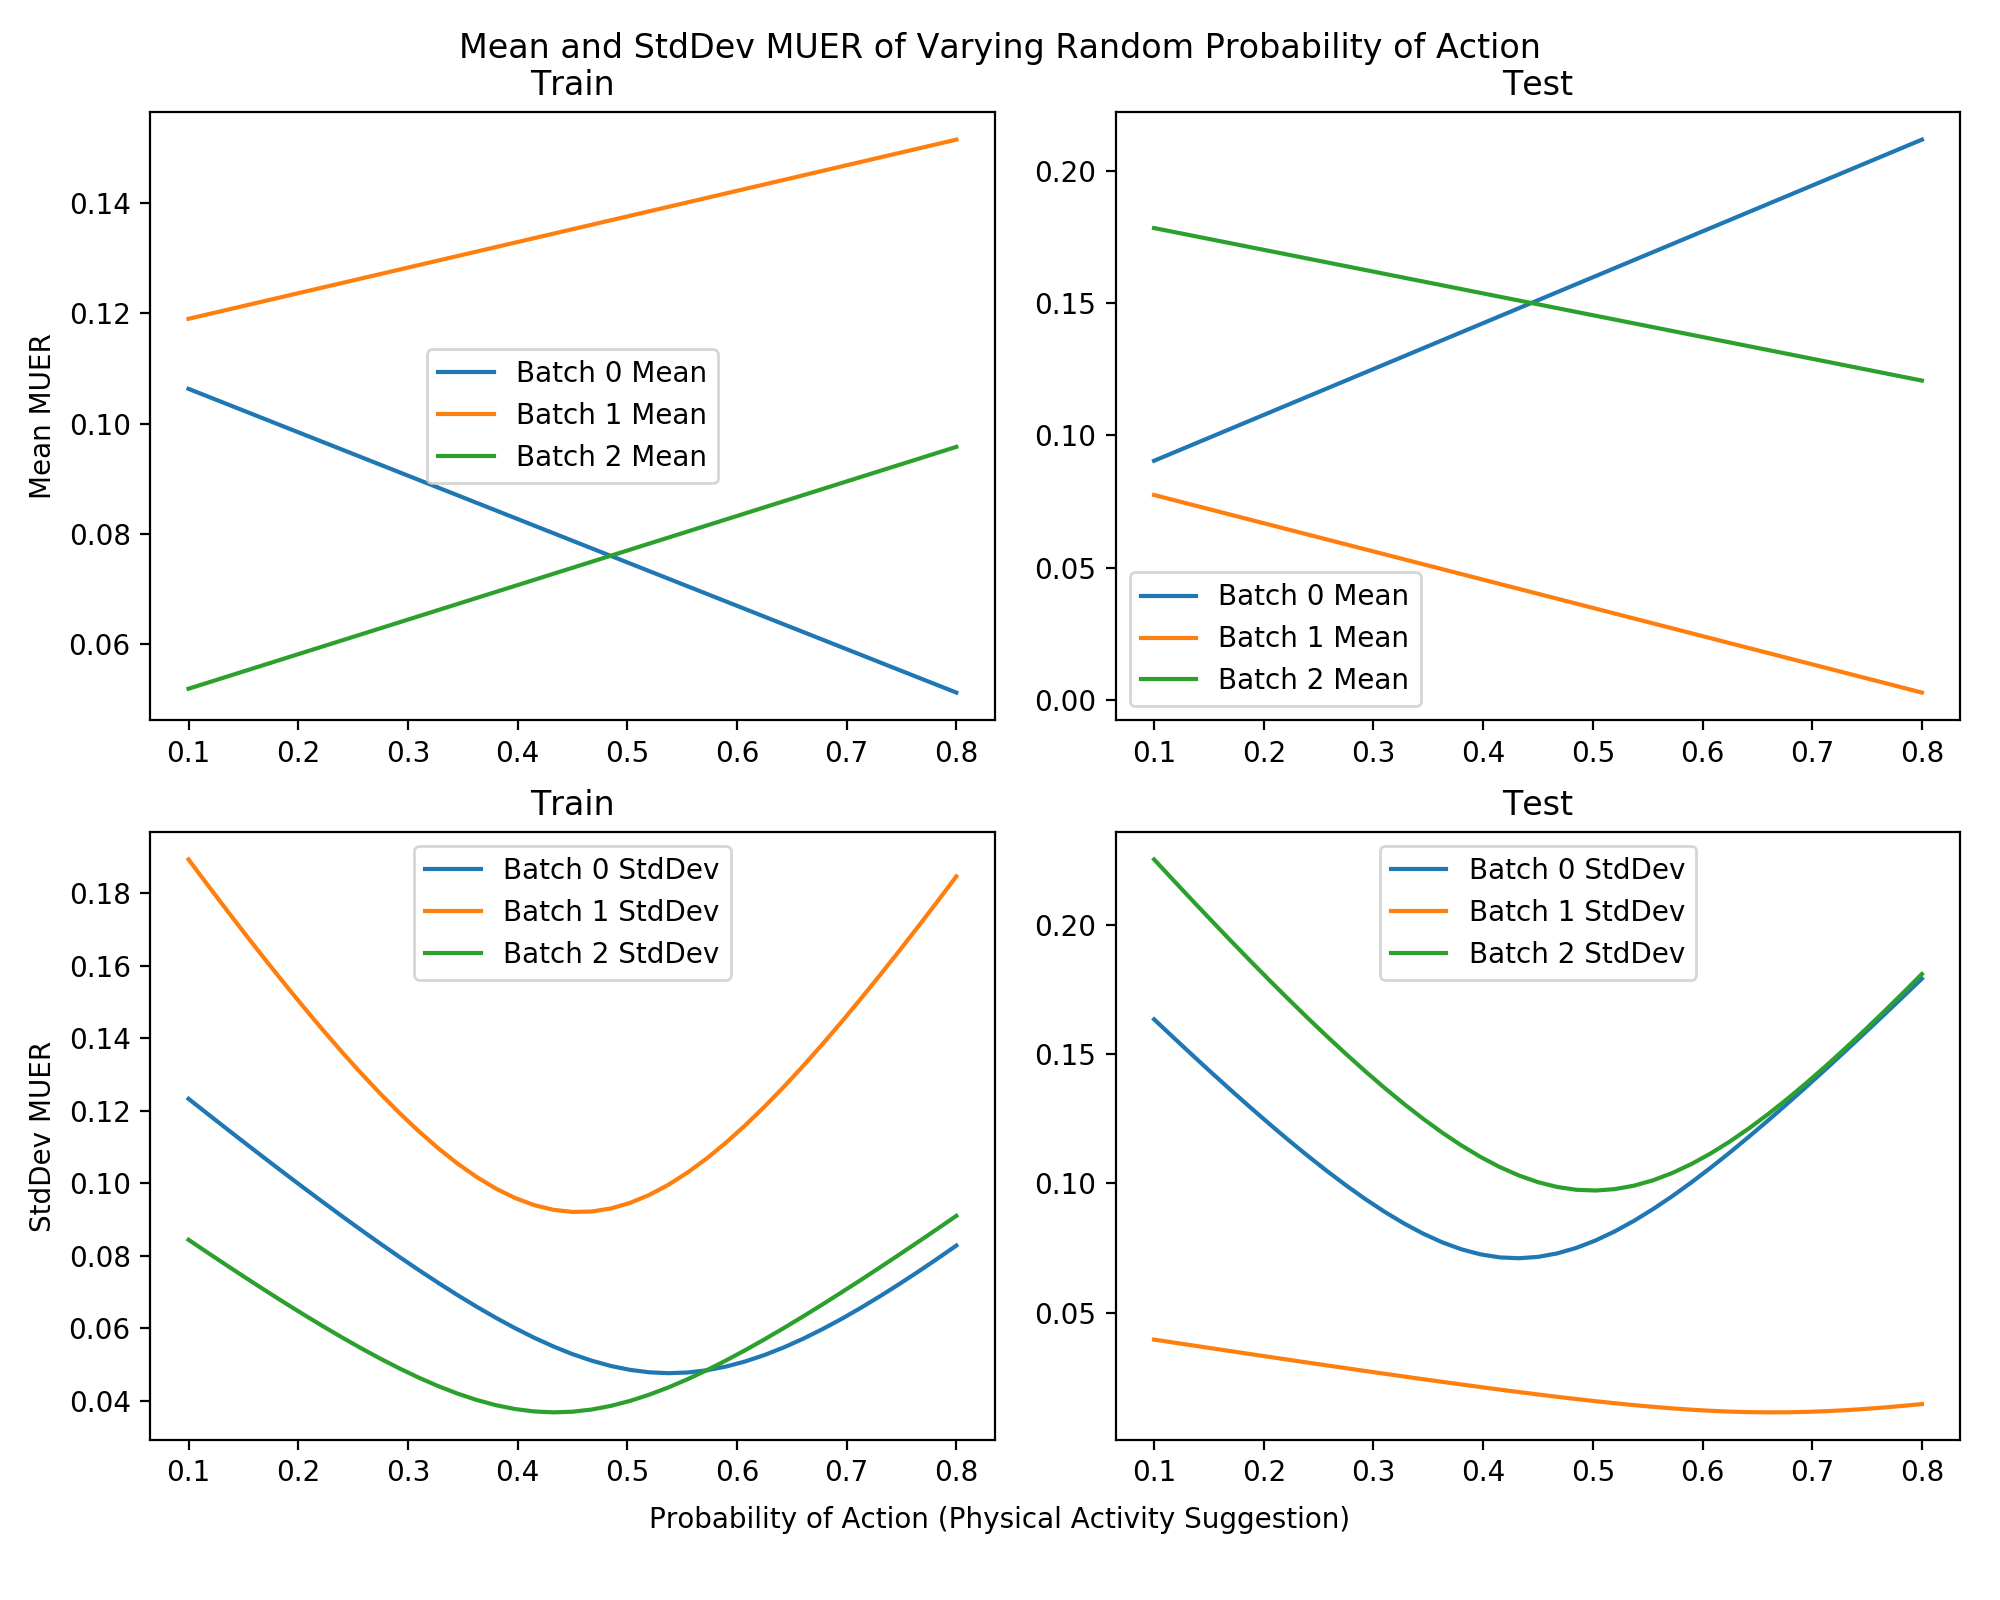
\includegraphics[width=0.8\textwidth,center]{figures/RandomActionVsProbability.png}}
\caption{Overall Regrets for Varying Action Probability $\pi_{(t,d)}$ vs $MUER$}
\label{RandomActionVsProbability}
\end{figure}


\begin{figure}[H]
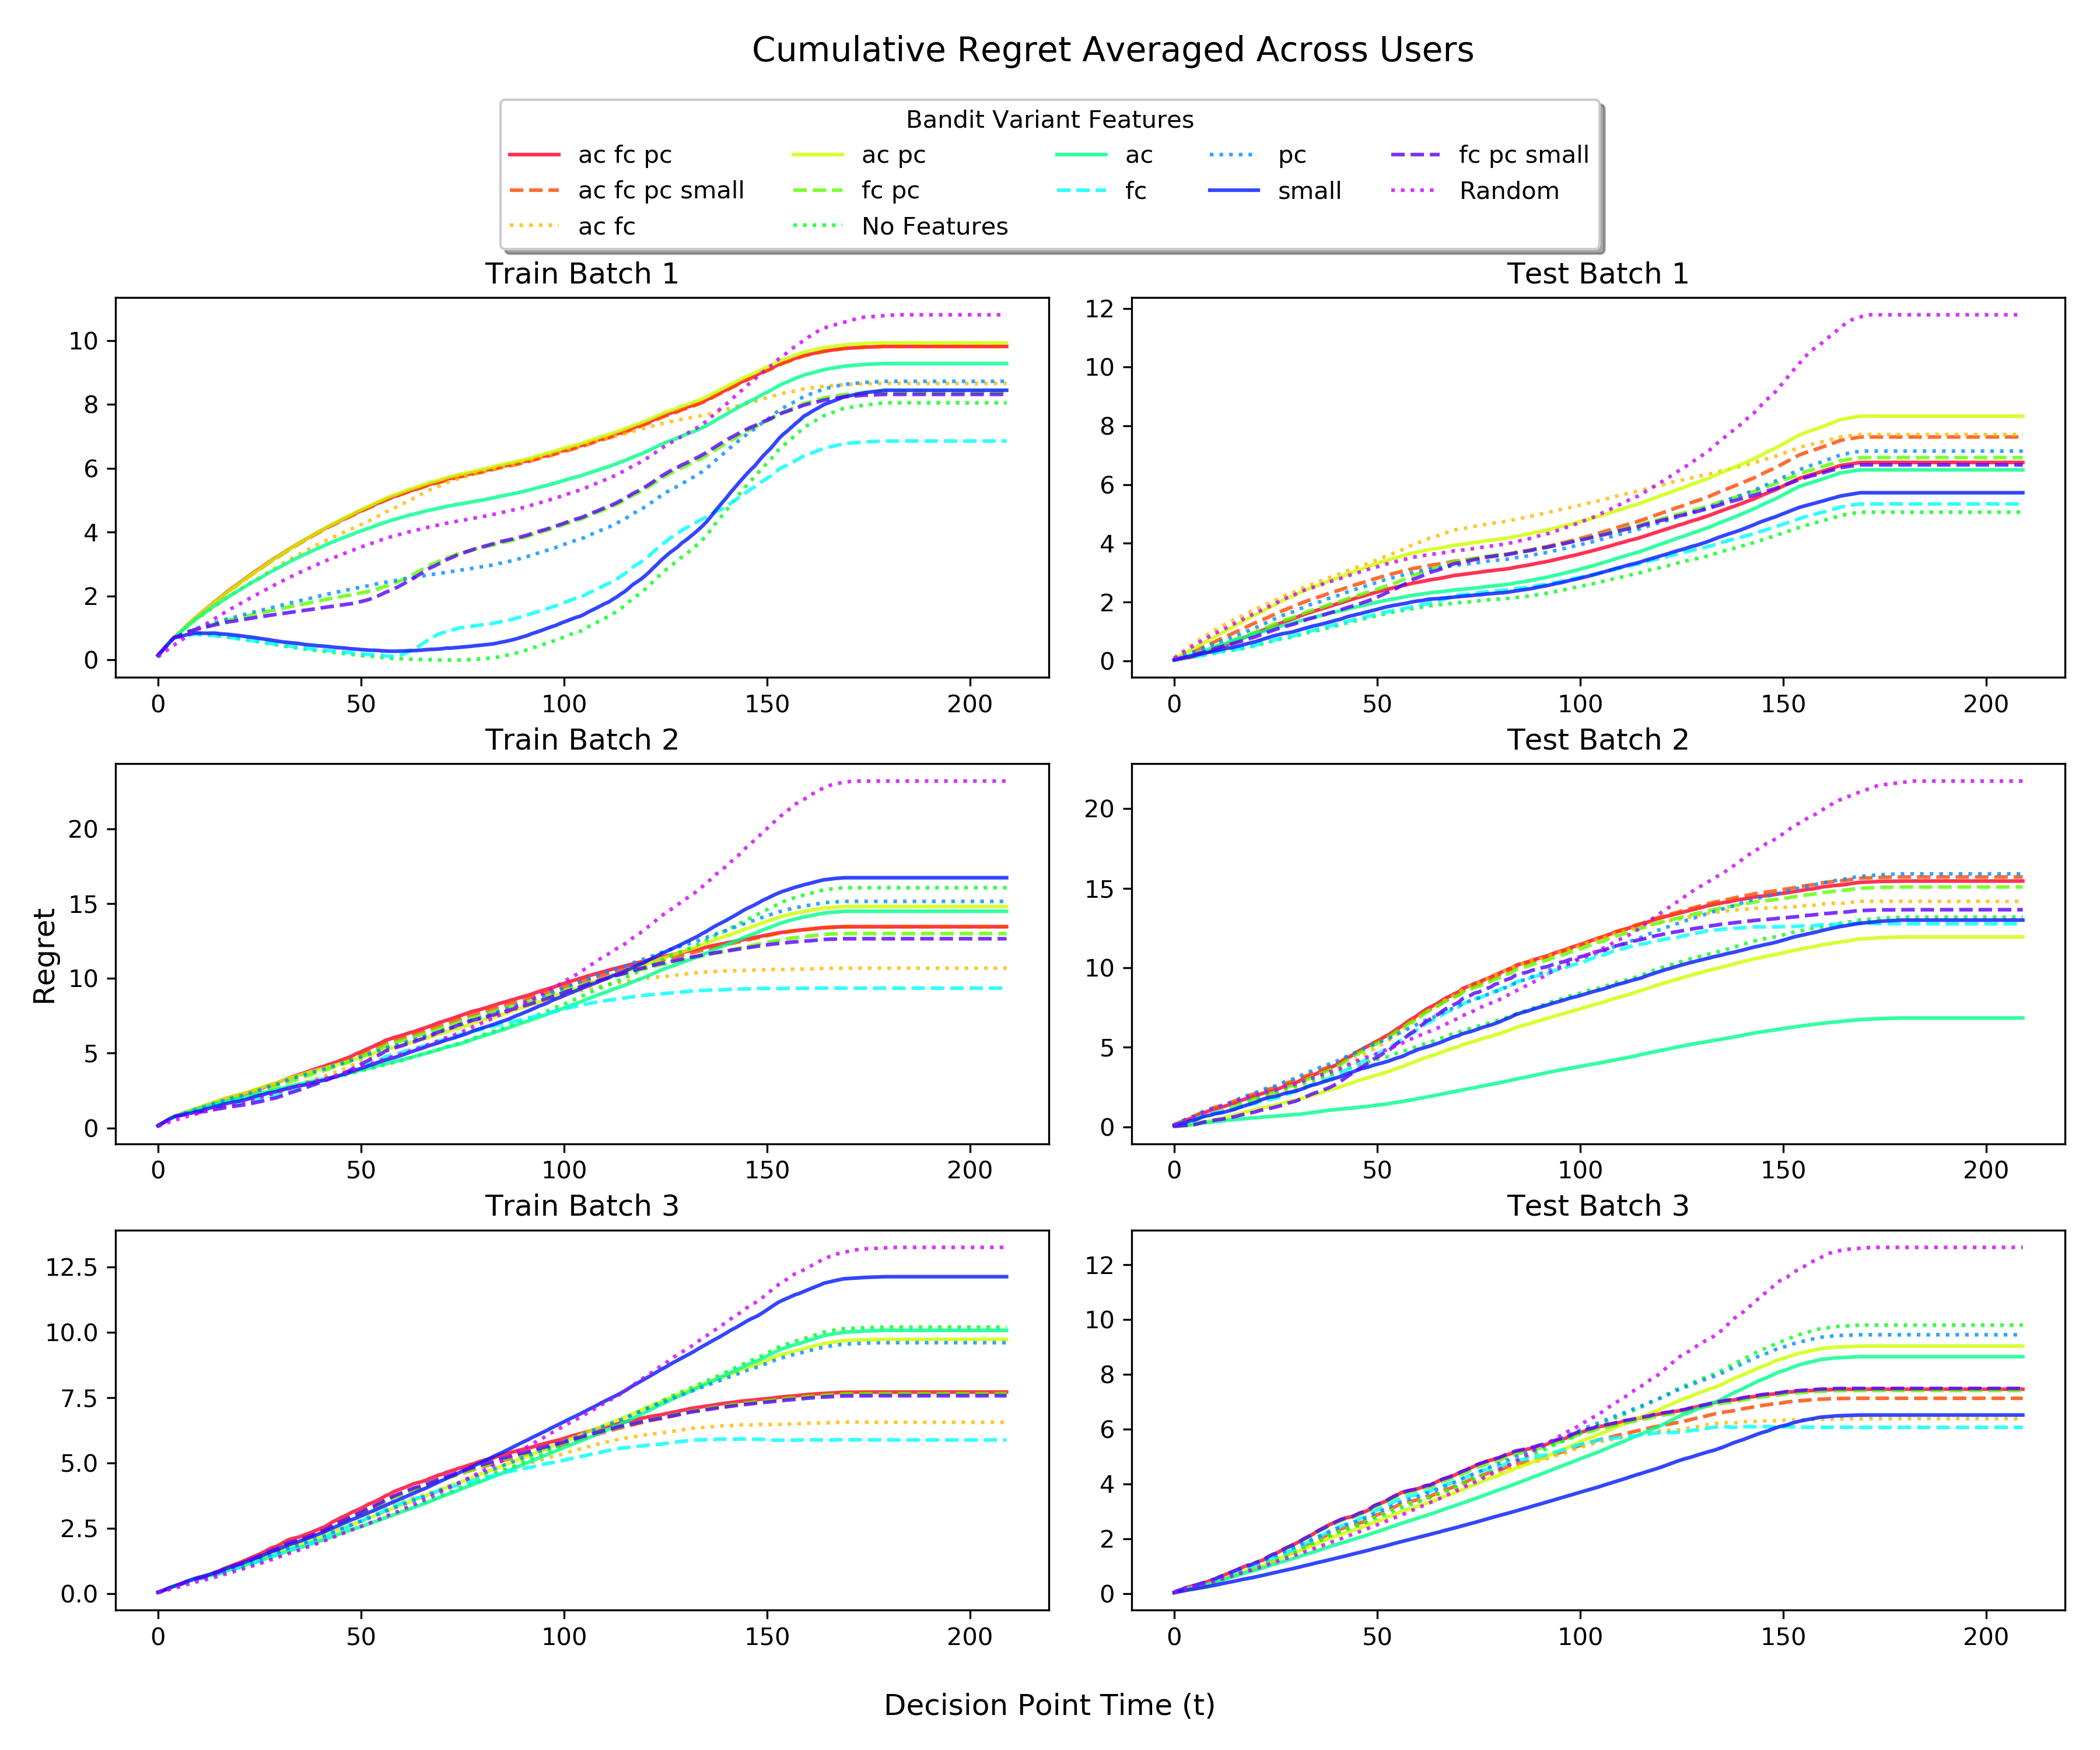
\includegraphics[width=1.35\textwidth,center]{figures/cum_regret_comparison.png}%
\caption{Cumulative Regrets for all Bandit Variants, Separated by Batch}
\label{Cumulative Regrets for all Bandit Variants, Separated by Batch}
\end{figure}

\clearpage

\section{Quality Metric Figures}
\label{Quality Metric Figures}

See additional {\bf Plots} folder to see Quality Metric Figures.  For each of the three batches $(1,2,3)$, the plots have been separated into Train and Test groups, for a total of $6$ total folders in the main {\bf Plots}.  Within each of the $6$ folders, there are $11$ subfolders, each named ``variant\_****'', where each of the * represent either $0$ or $1$; these are results for each variant of the Bandit for one of the three train/test batches.

\begin{itemize}
	\item The first number indicates the use of action centering (ac); $1$ indicates that ac was used, $0$ indicates ac was not used.
	\item The second number indicates the use of a feedback controller (fc); $1$ means on, $0$ means off.
	\item The third number indicates the use of probability clipping (pc); $1$ means on, $0$ means off.
	\item The fourth number indicates the use of the Small model (small); $0$ means that the Full model was used, and $1$ means that the Small model was used.
\end{itemize}

Inside each subfolder, there are $19$ Quality Metric plots, all of whose descriptions can be found in table \ref{QM Table}.



\section{Parameter Tuning vs MUER Figures}



In this section, we present the effect of varying values of the tuning parameters on $MUER$ mean and standard deviation, for the standard bandit (ac fc pc), with optimization using $MUER$ mean minimization as well as using the StdDev cutoff method.  For each optimization method, there are $4$ figures, corresponding with the number of times we cycled through all of the tuning parameters performing a parameter sweep optimization.  \\

Within each figure are two plots.  The first plot shows the $MUER$ mean, along with a red dashed line of best linear fit, with the fitted line's equation printed in red.  The second plot shows the $MUER$ standard deviation.  In both plots, the chosen value of the parameter is given by the vertical purple dotted line, whether by $MUER$ mean minimization or using a StdDev cutoff.  

All parameters were tuned in the given range from table \ref{Parameter Optimization Table}, with $160$ steps in between ($160$ chosen to leverage available dedicated \href{https://www.rc.fas.harvard.edu/}{Odyssey Research} cluster computing cores in parallel computation).  


% \subsection{$MUER$ Minimization Parameter Optimization}
\label{MUER Minimization Parameter Optimization}


	\ifdraft
	Turn off Draft mode to display figures!
	\else
	%%%%%%%%%%%%%%%%%%%%%%%%%%%%%%%%%%%%%%%%%%%%%%%%%%%%%%%%%%%%%%%%%%%%%
	\begin{figure}[H]
	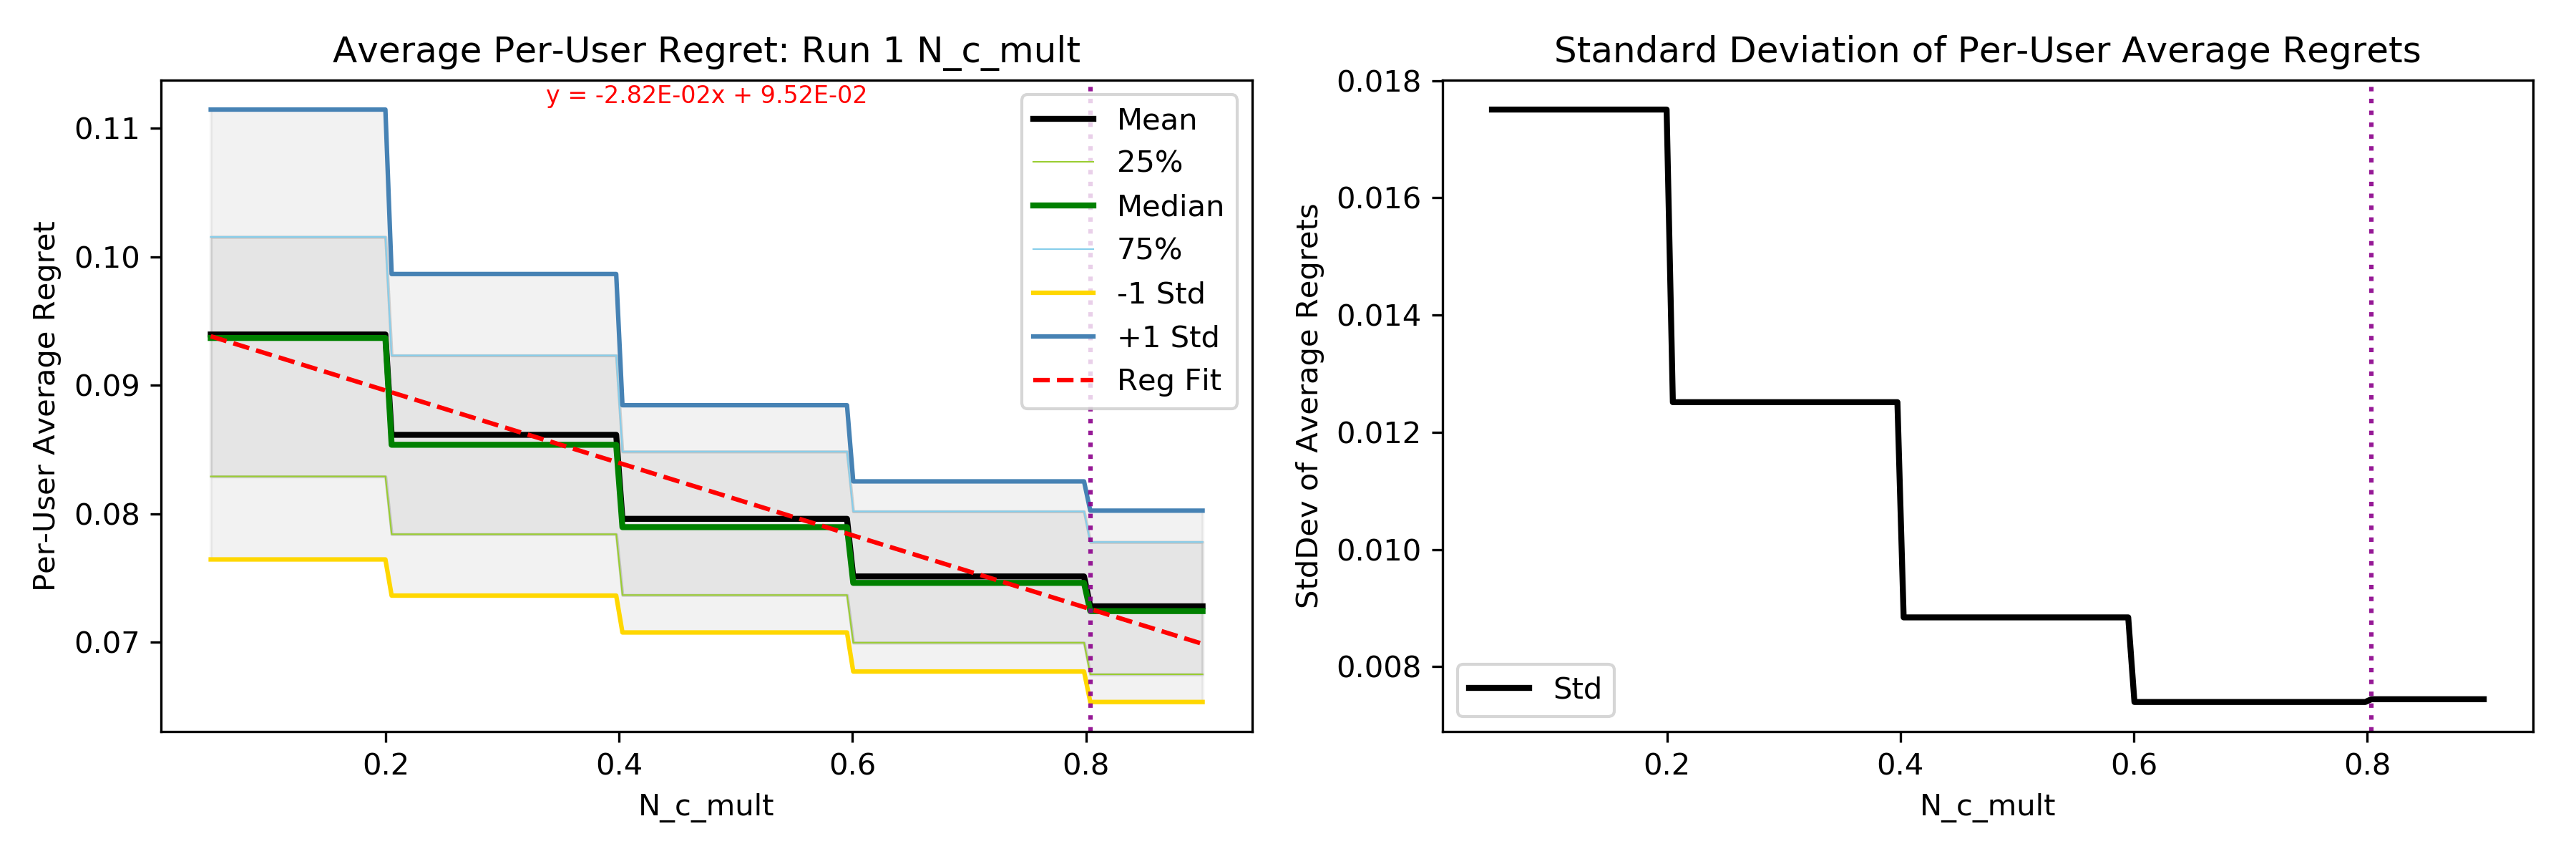
\includegraphics[width=1.1\textwidth,center]{figures/opt_param/opt_param_11100_N_c_mult1.png}%
	\newline
	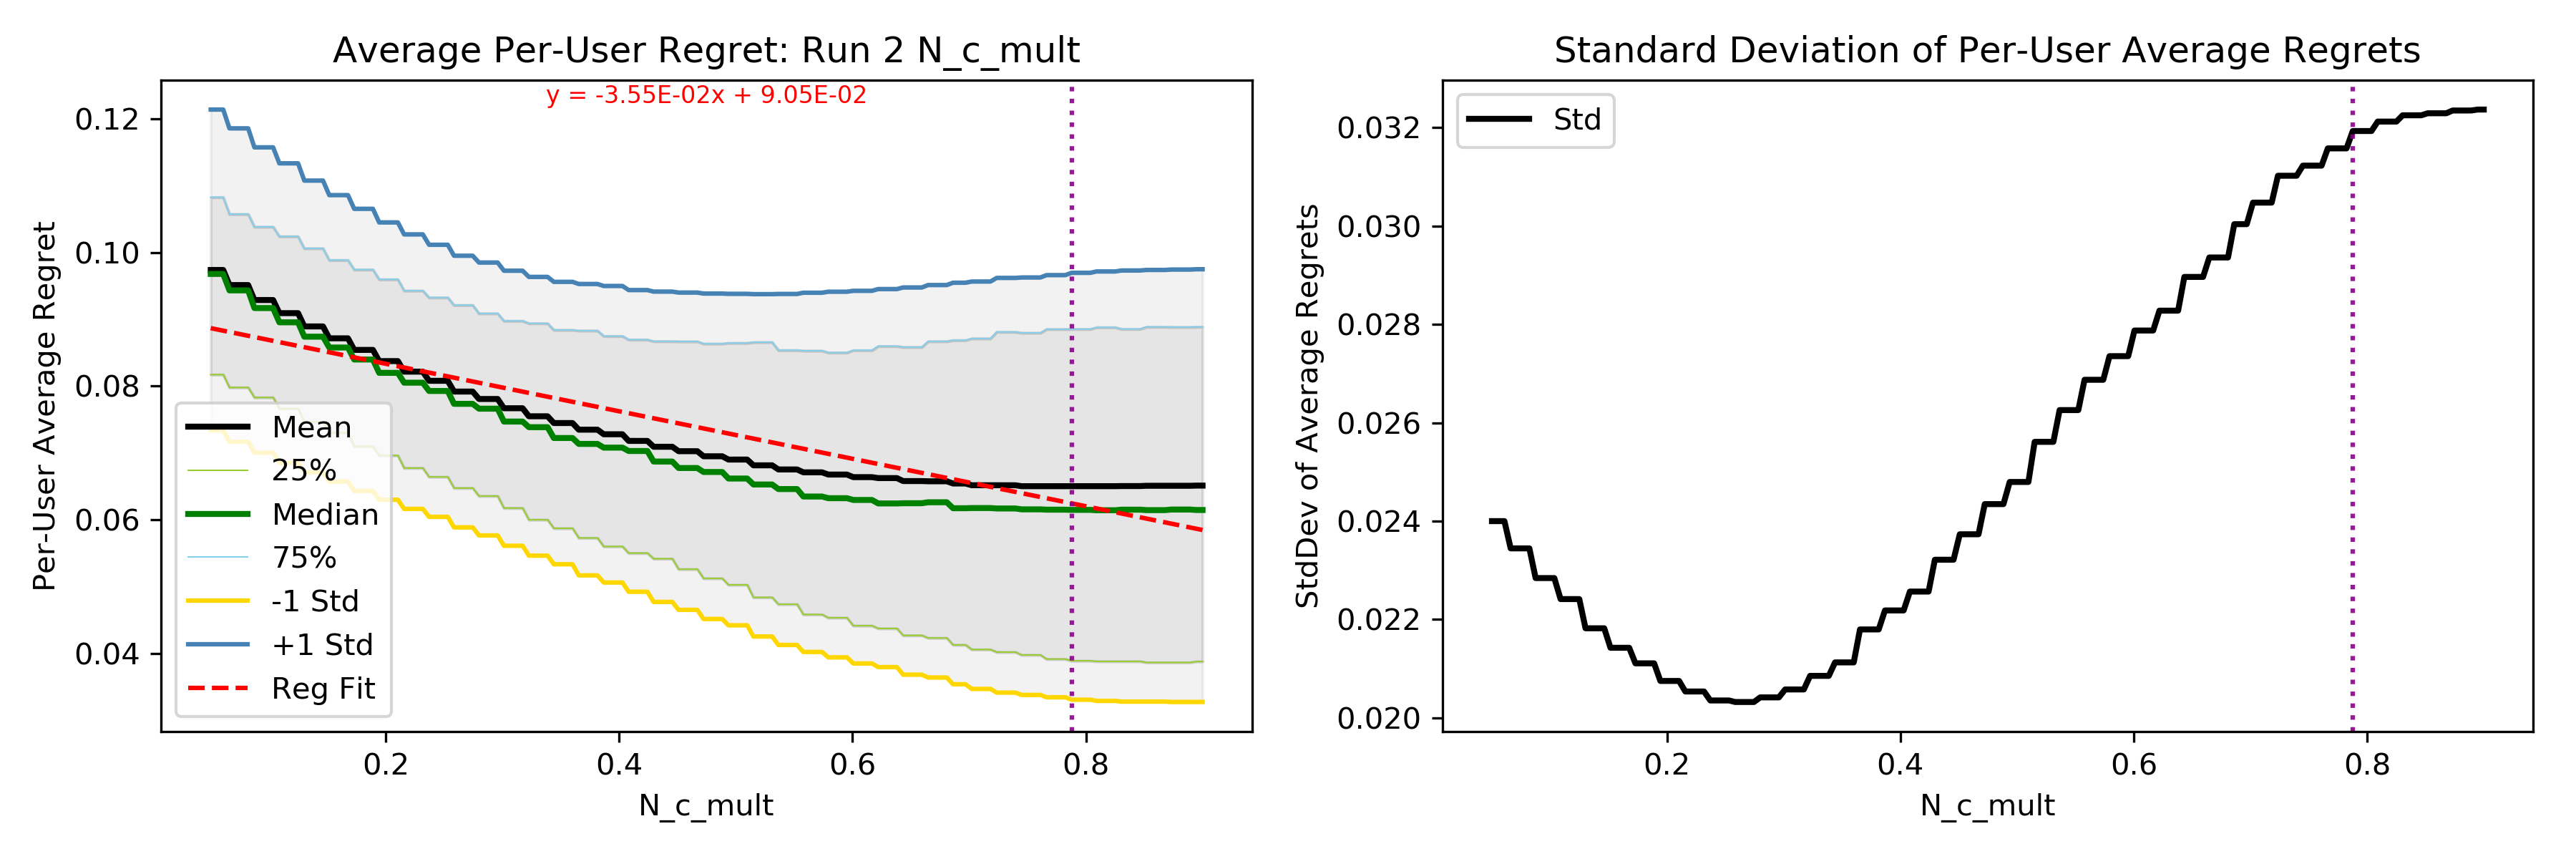
\includegraphics[width=1.1\textwidth,center]{figures/opt_param/opt_param_11100_N_c_mult2.png}%
	\newline
	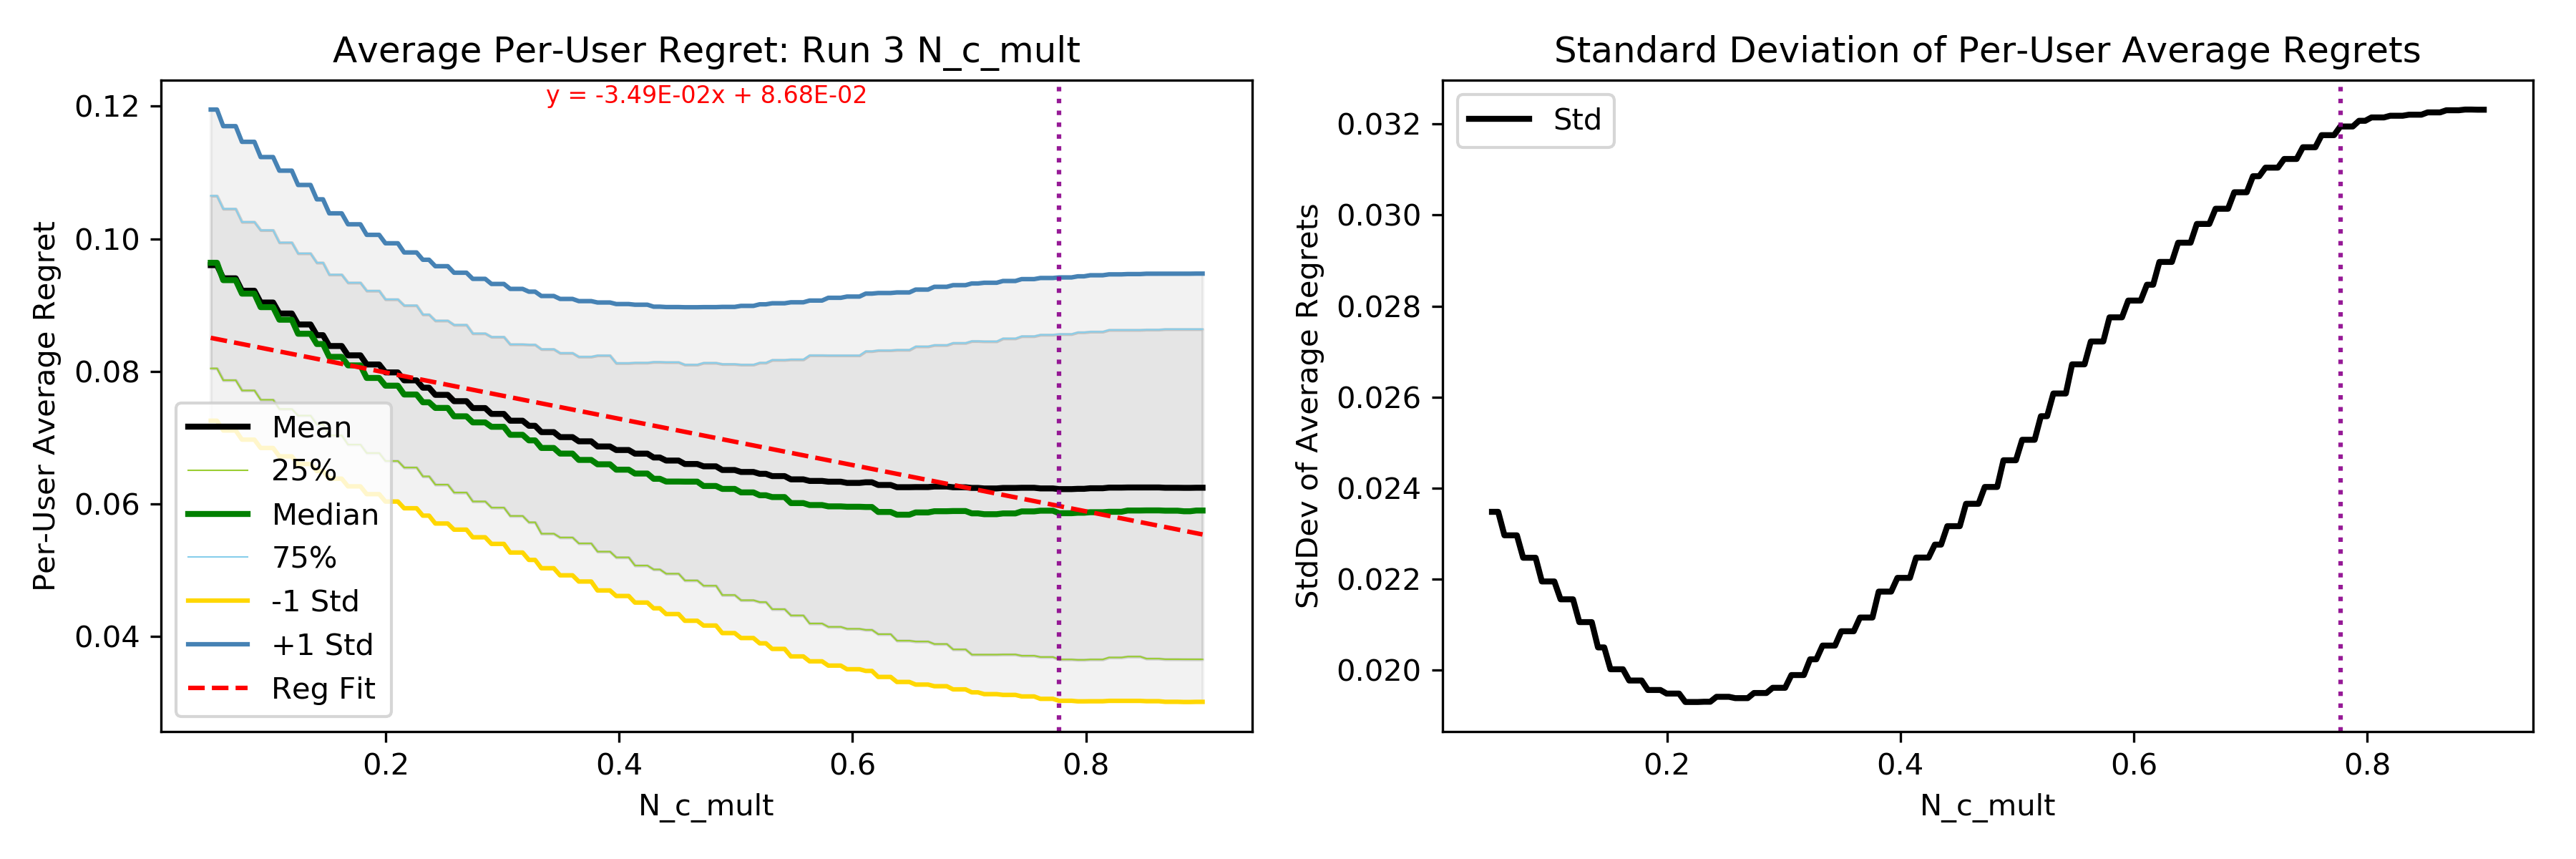
\includegraphics[width=1.1\textwidth,center]{figures/opt_param/opt_param_11100_N_c_mult3.png}%
	\newline
	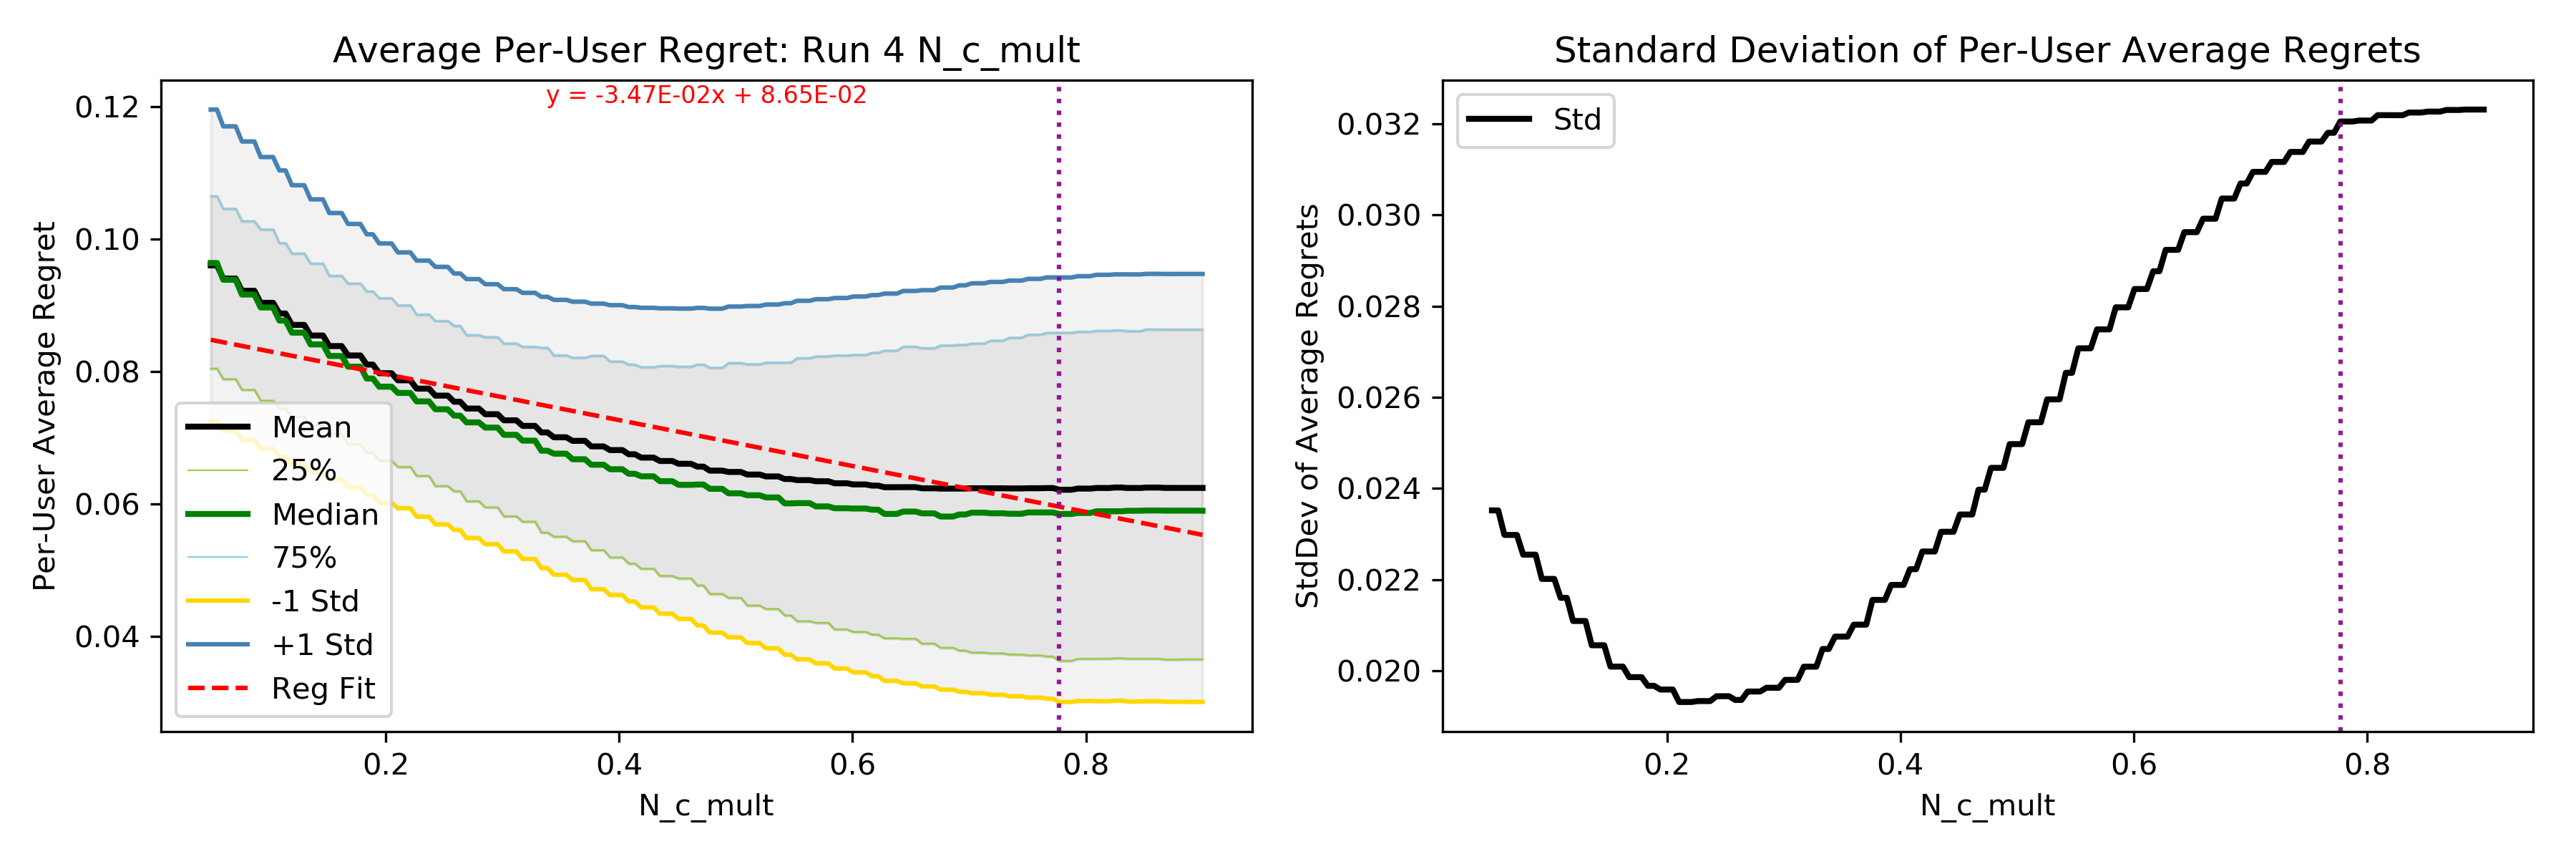
\includegraphics[width=1.1\textwidth,center]{figures/opt_param/opt_param_11100_N_c_mult4.png}%
	\caption{$MUER$ for Varying $\mathtt{N\_c\_mult}$, $MUER$ Minimization Optimization}
	\end{figure}

	\begin{figure}[H]
	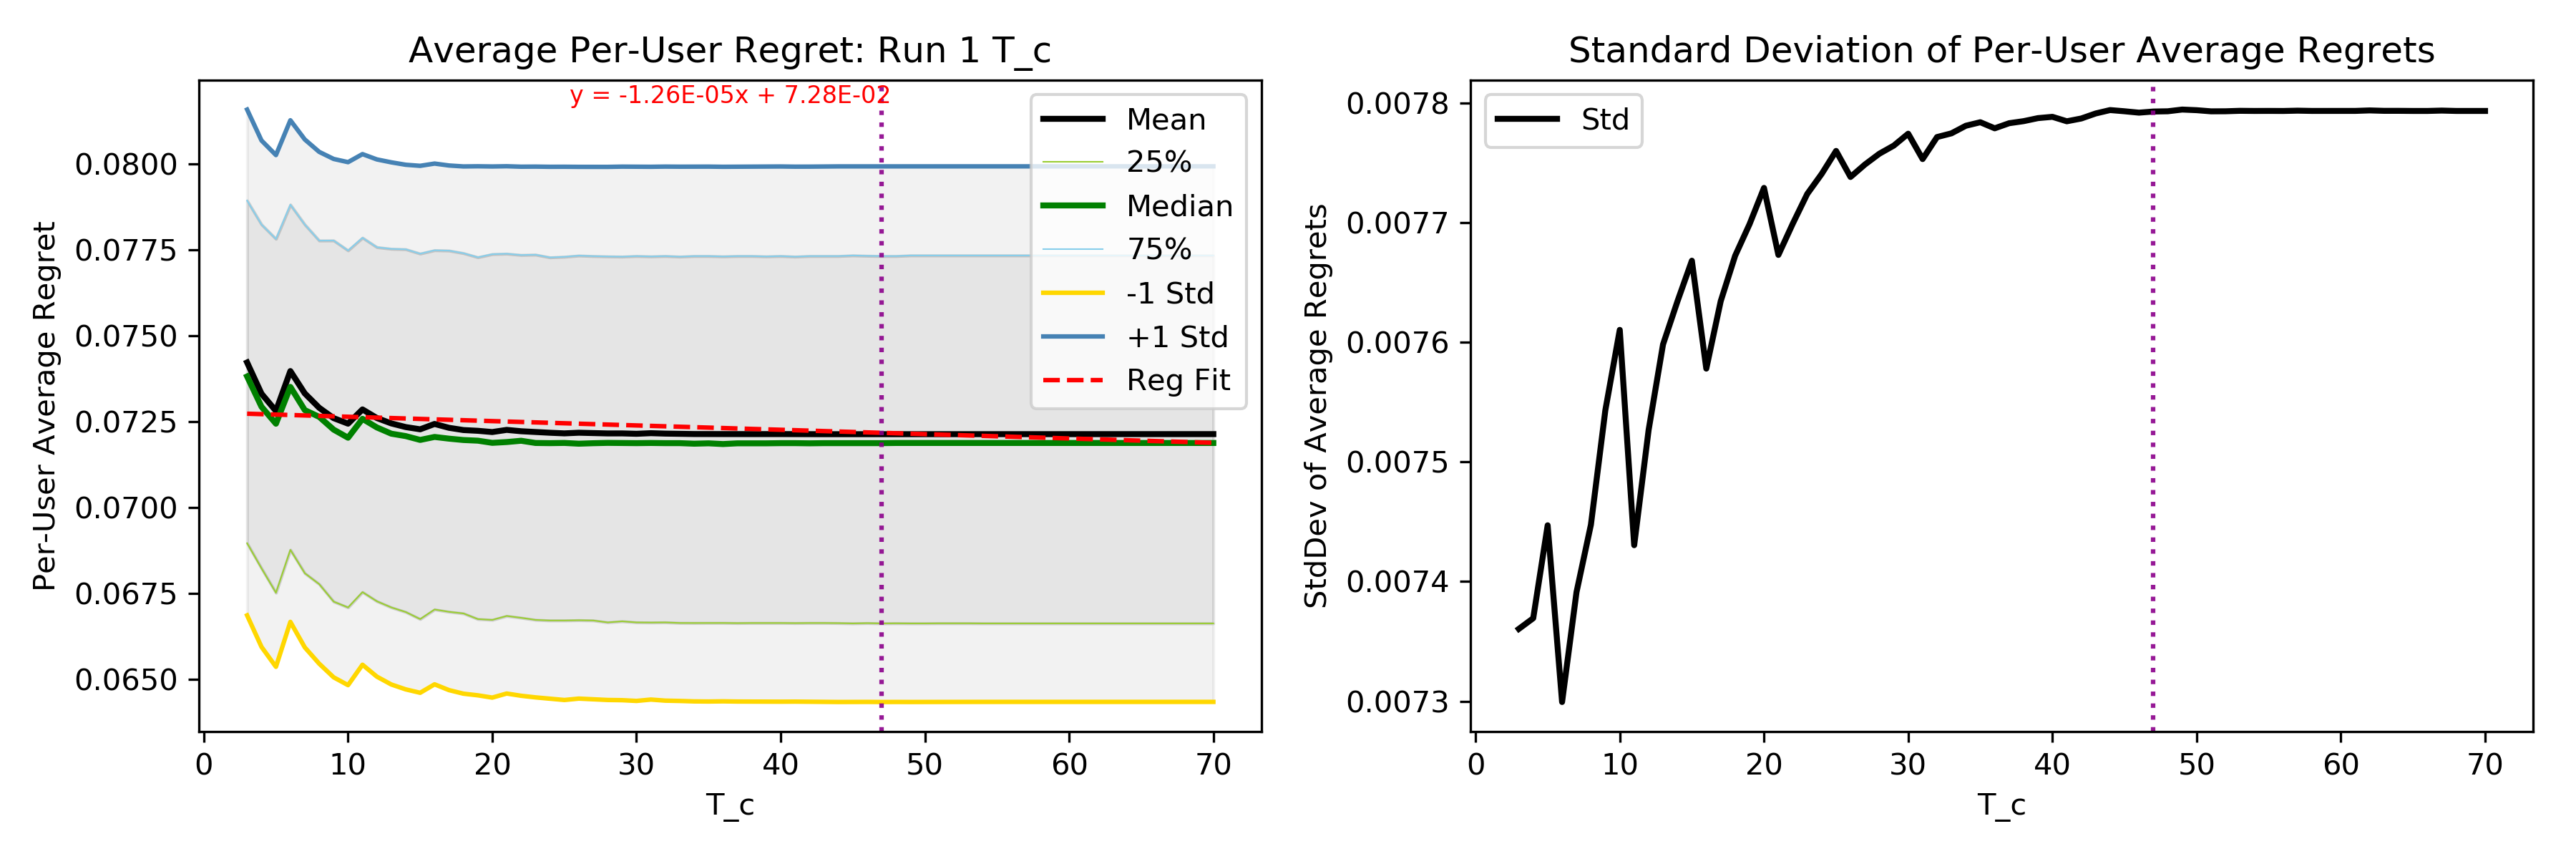
\includegraphics[width=1.1\textwidth,center]{figures/opt_param/opt_param_11100_T_c1.png}%
	\newline
	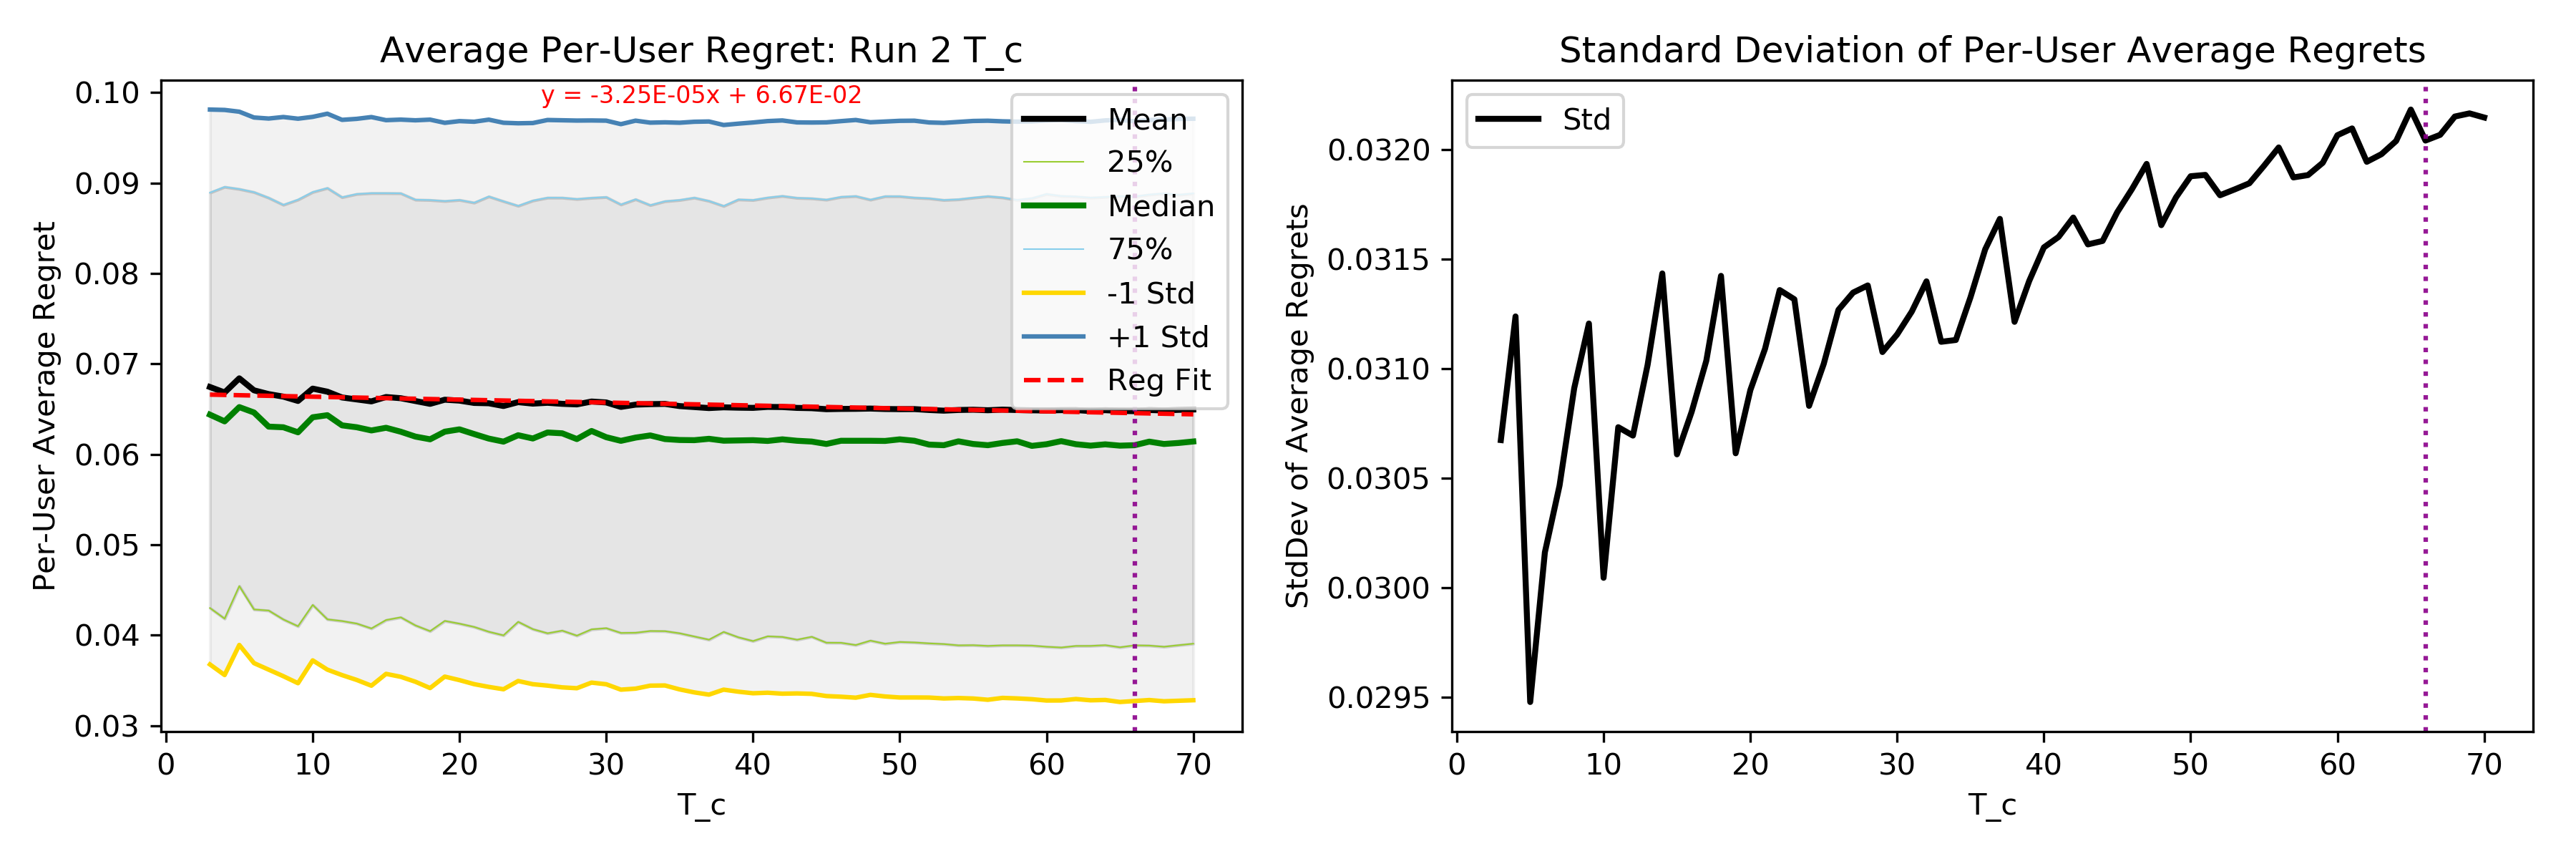
\includegraphics[width=1.1\textwidth,center]{figures/opt_param/opt_param_11100_T_c2.png}%
	\newline
	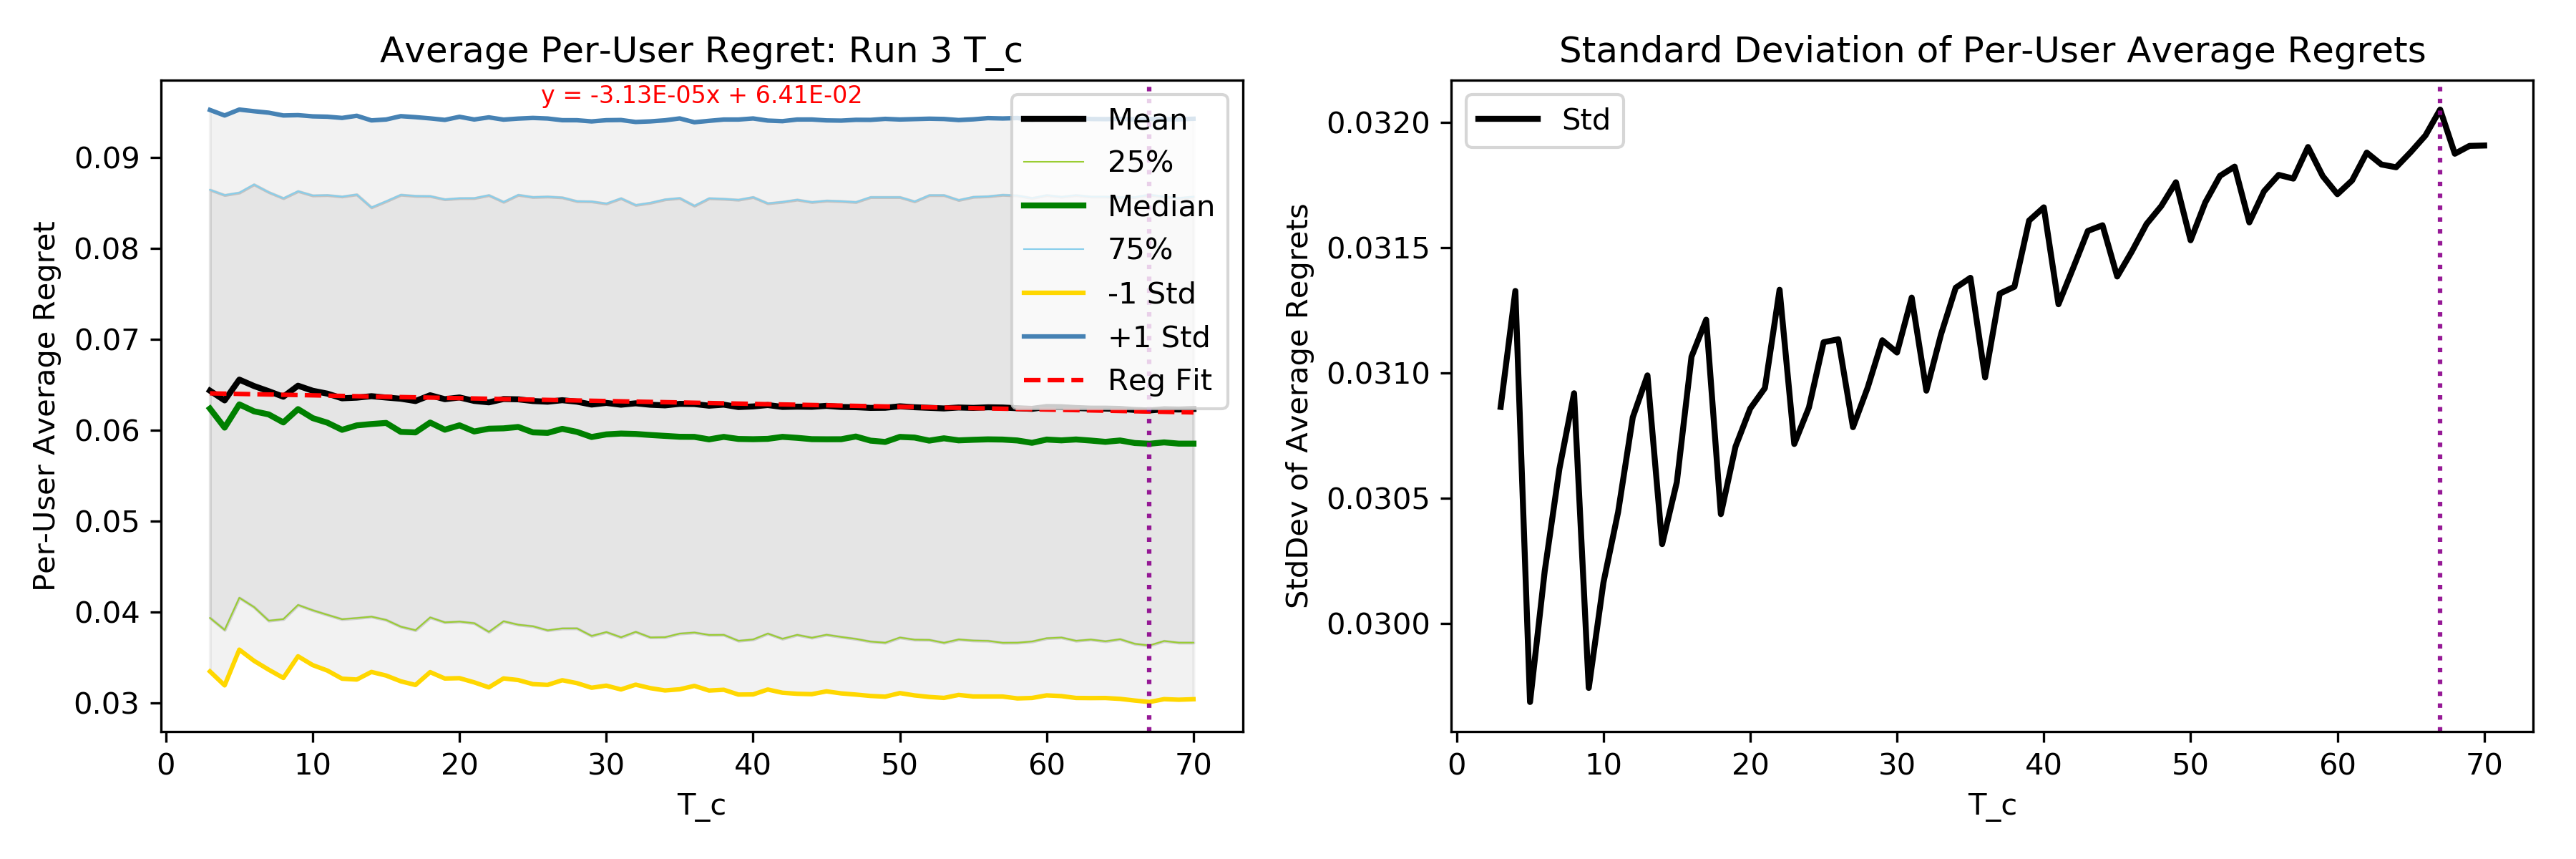
\includegraphics[width=1.1\textwidth,center]{figures/opt_param/opt_param_11100_T_c3.png}%
	\newline
	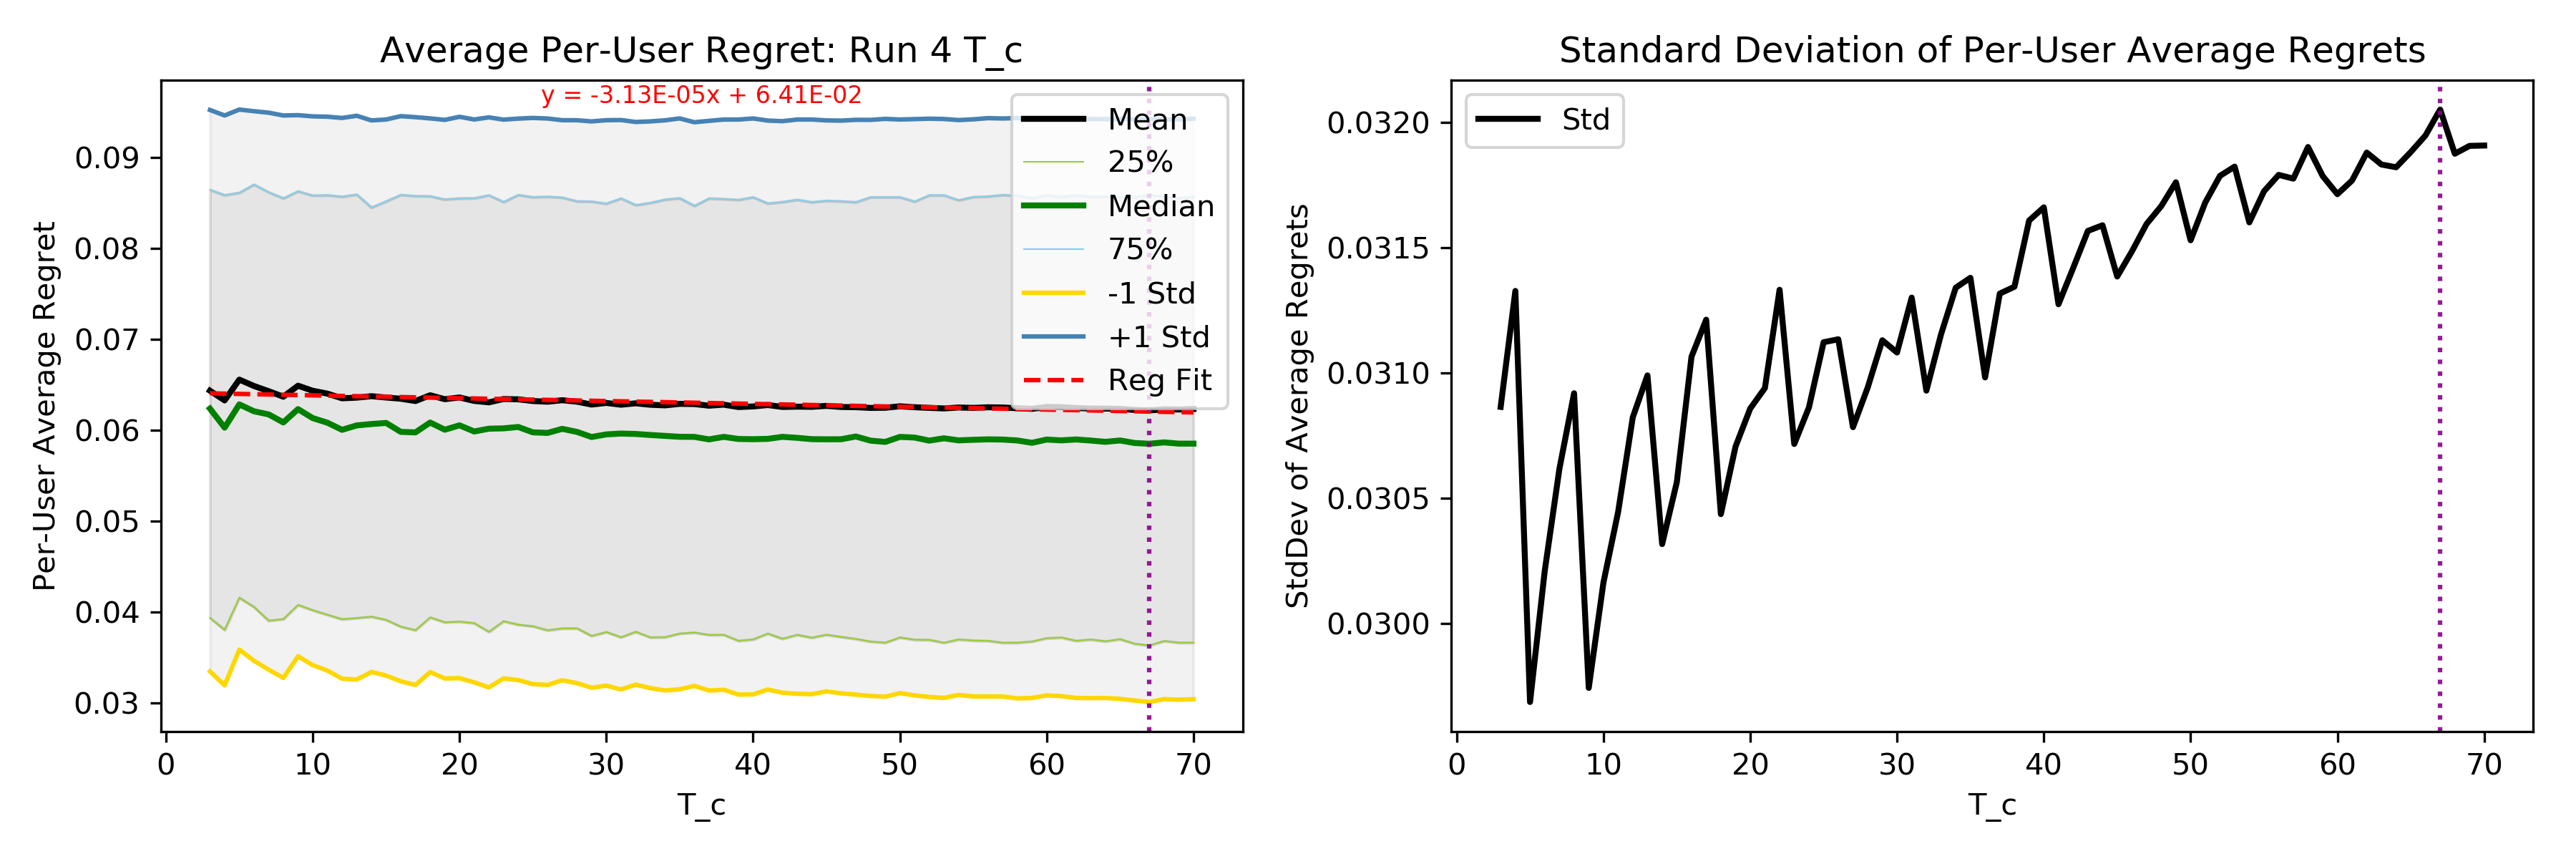
\includegraphics[width=1.1\textwidth,center]{figures/opt_param/opt_param_11100_T_c4.png}%
	\caption{$MUER$ for Varying $\mathtt{T\_c}$, $MUER$ Minimization Optimization}
	\end{figure}

	\begin{figure}[H]
	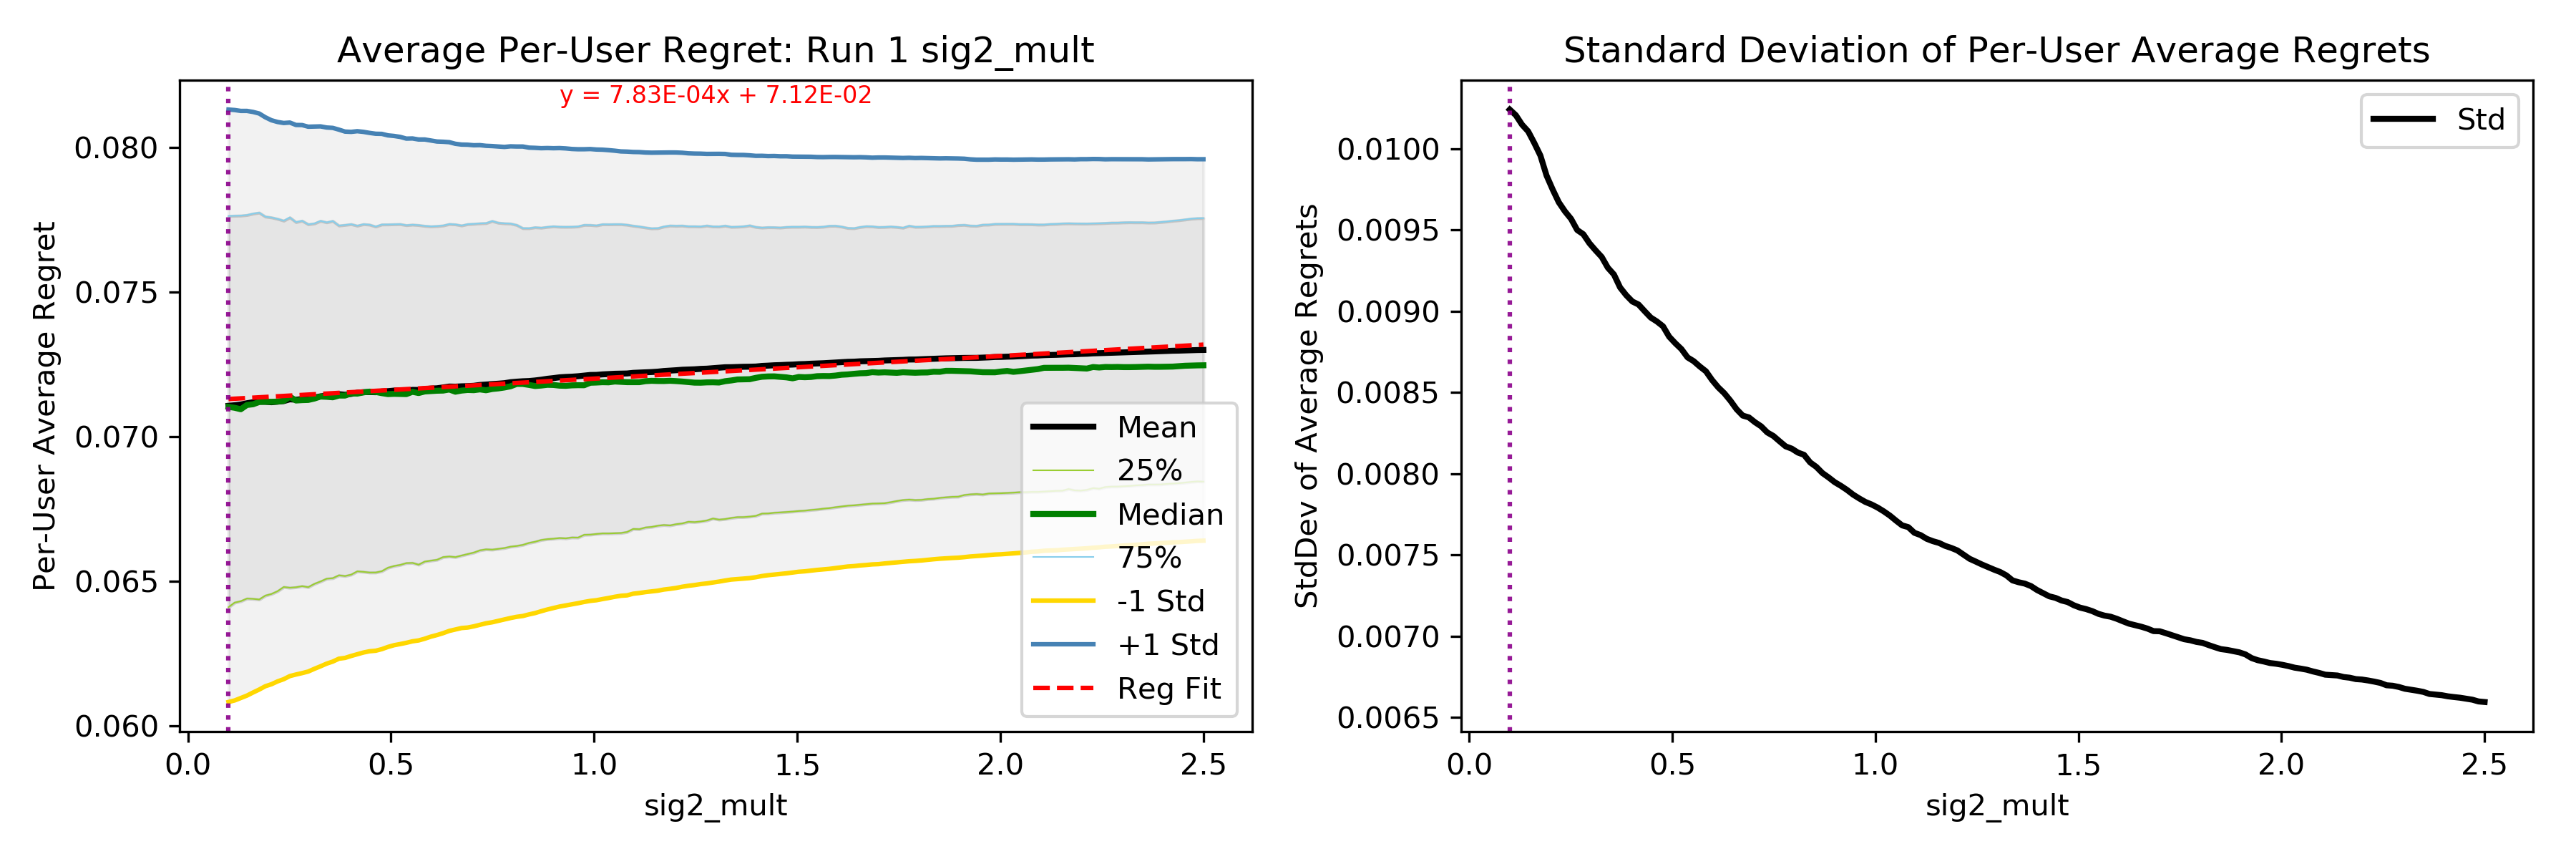
\includegraphics[width=1.1\textwidth,center]{figures/opt_param/opt_param_11100_sig2_mult1.png}%
	\newline
	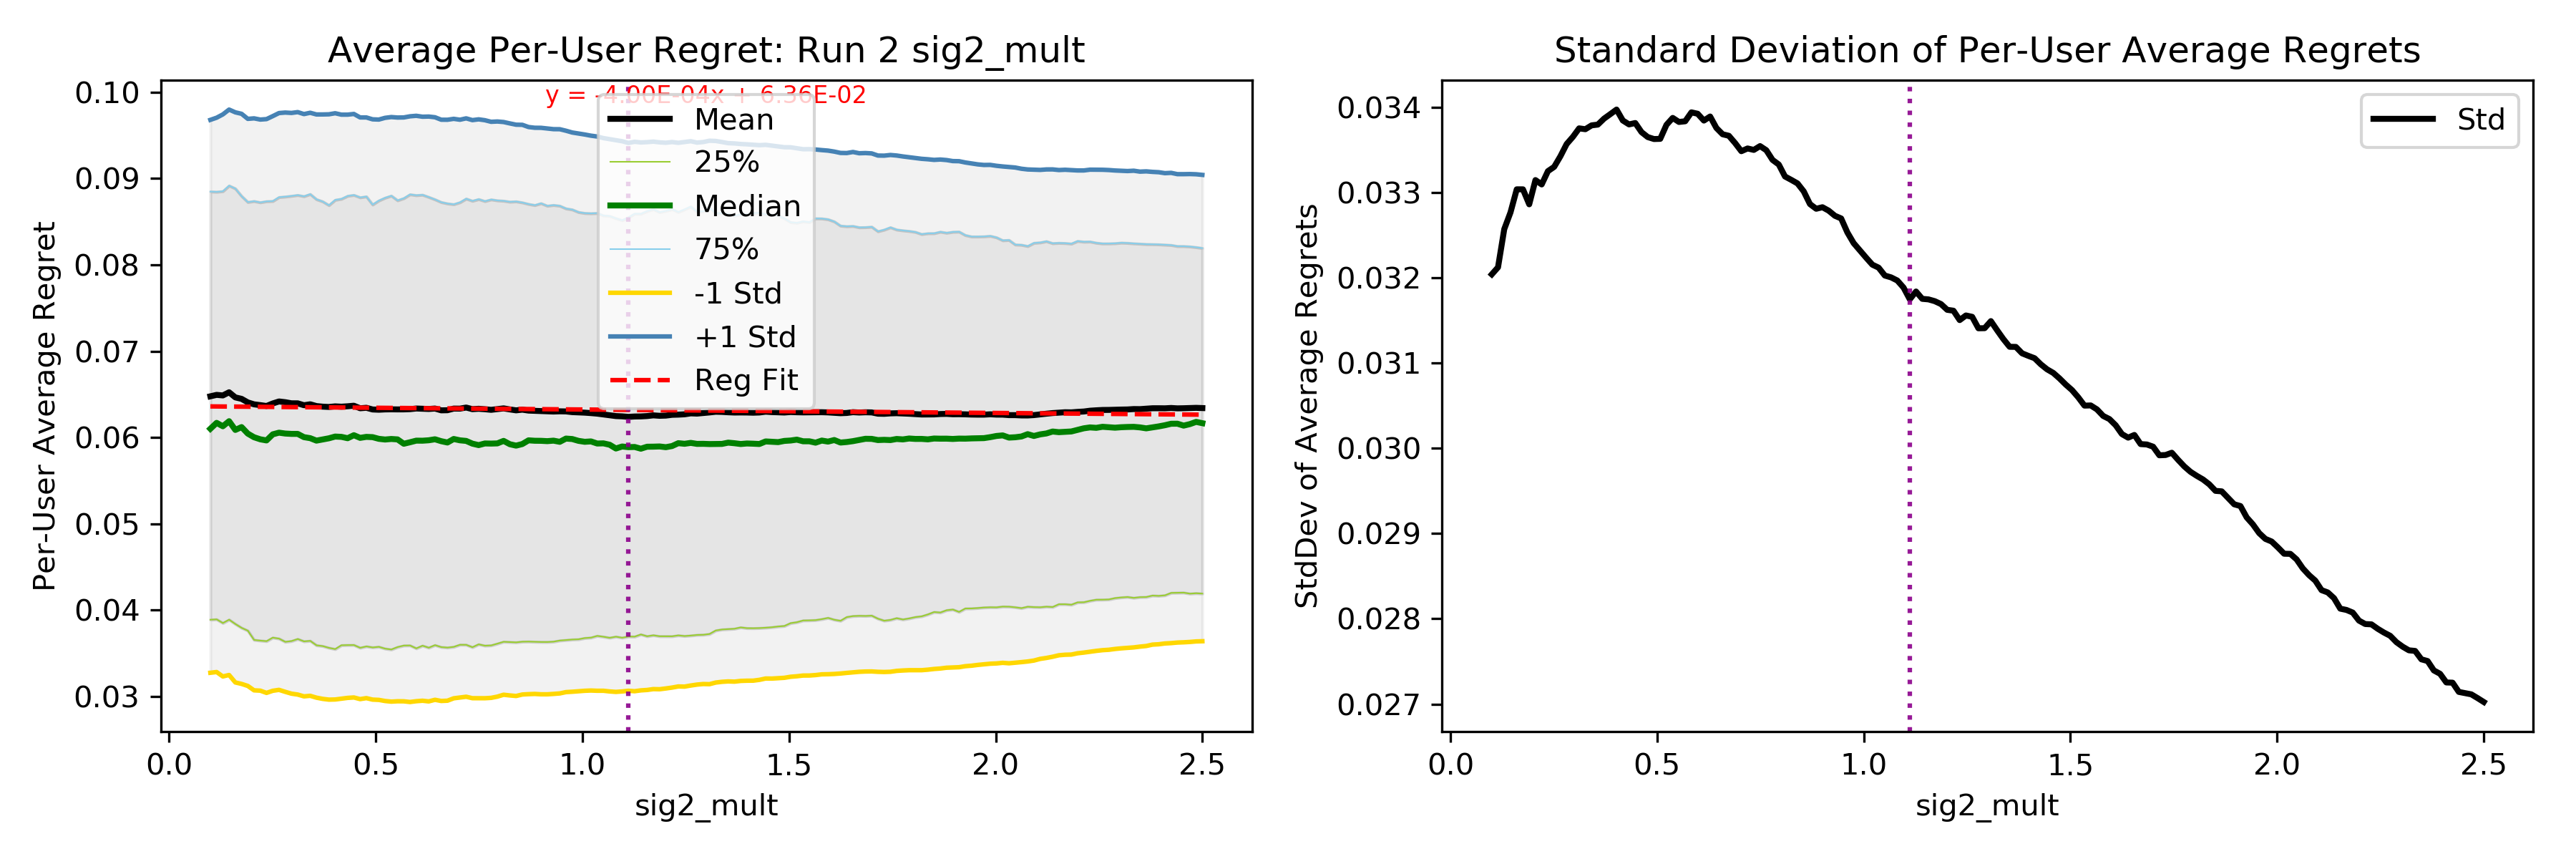
\includegraphics[width=1.1\textwidth,center]{figures/opt_param/opt_param_11100_sig2_mult2.png}%
	\newline
	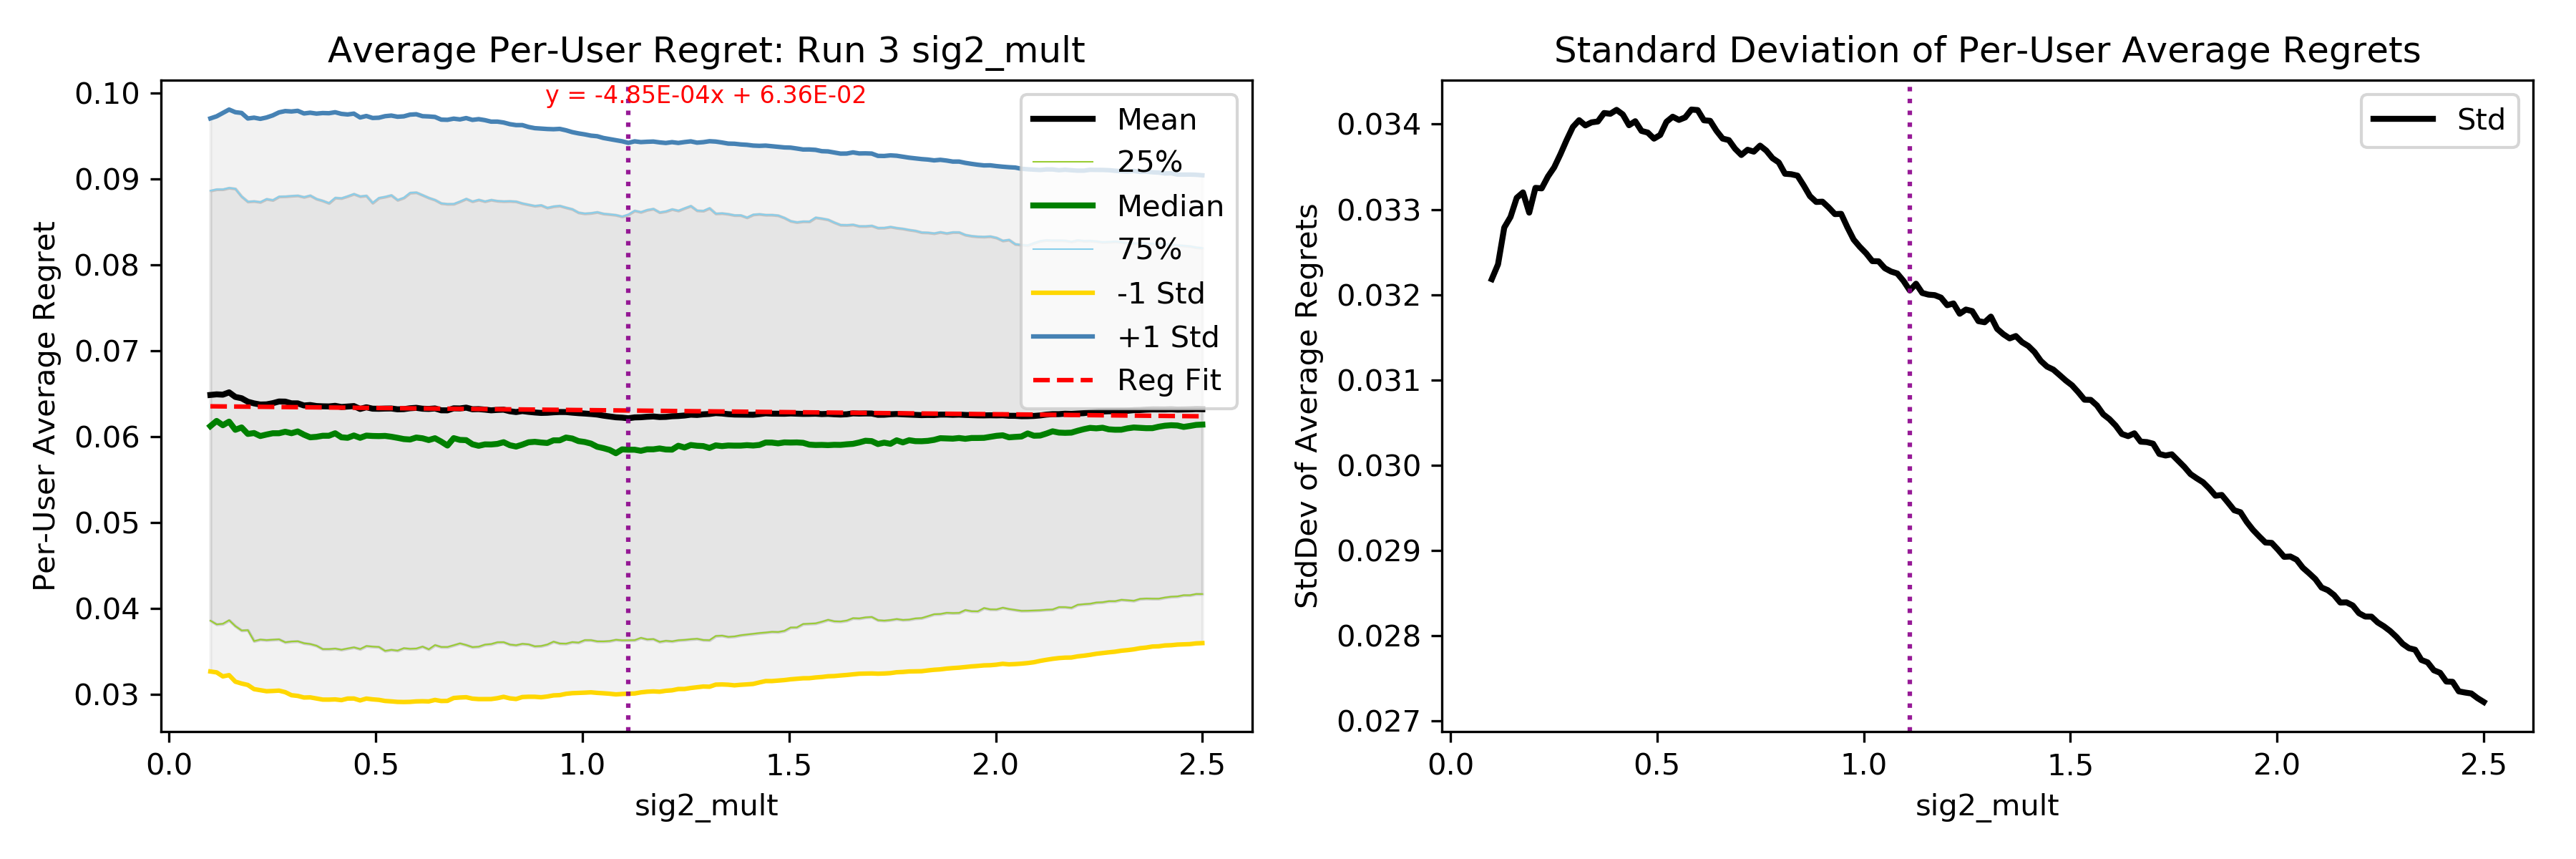
\includegraphics[width=1.1\textwidth,center]{figures/opt_param/opt_param_11100_sig2_mult3.png}%
	\newline
	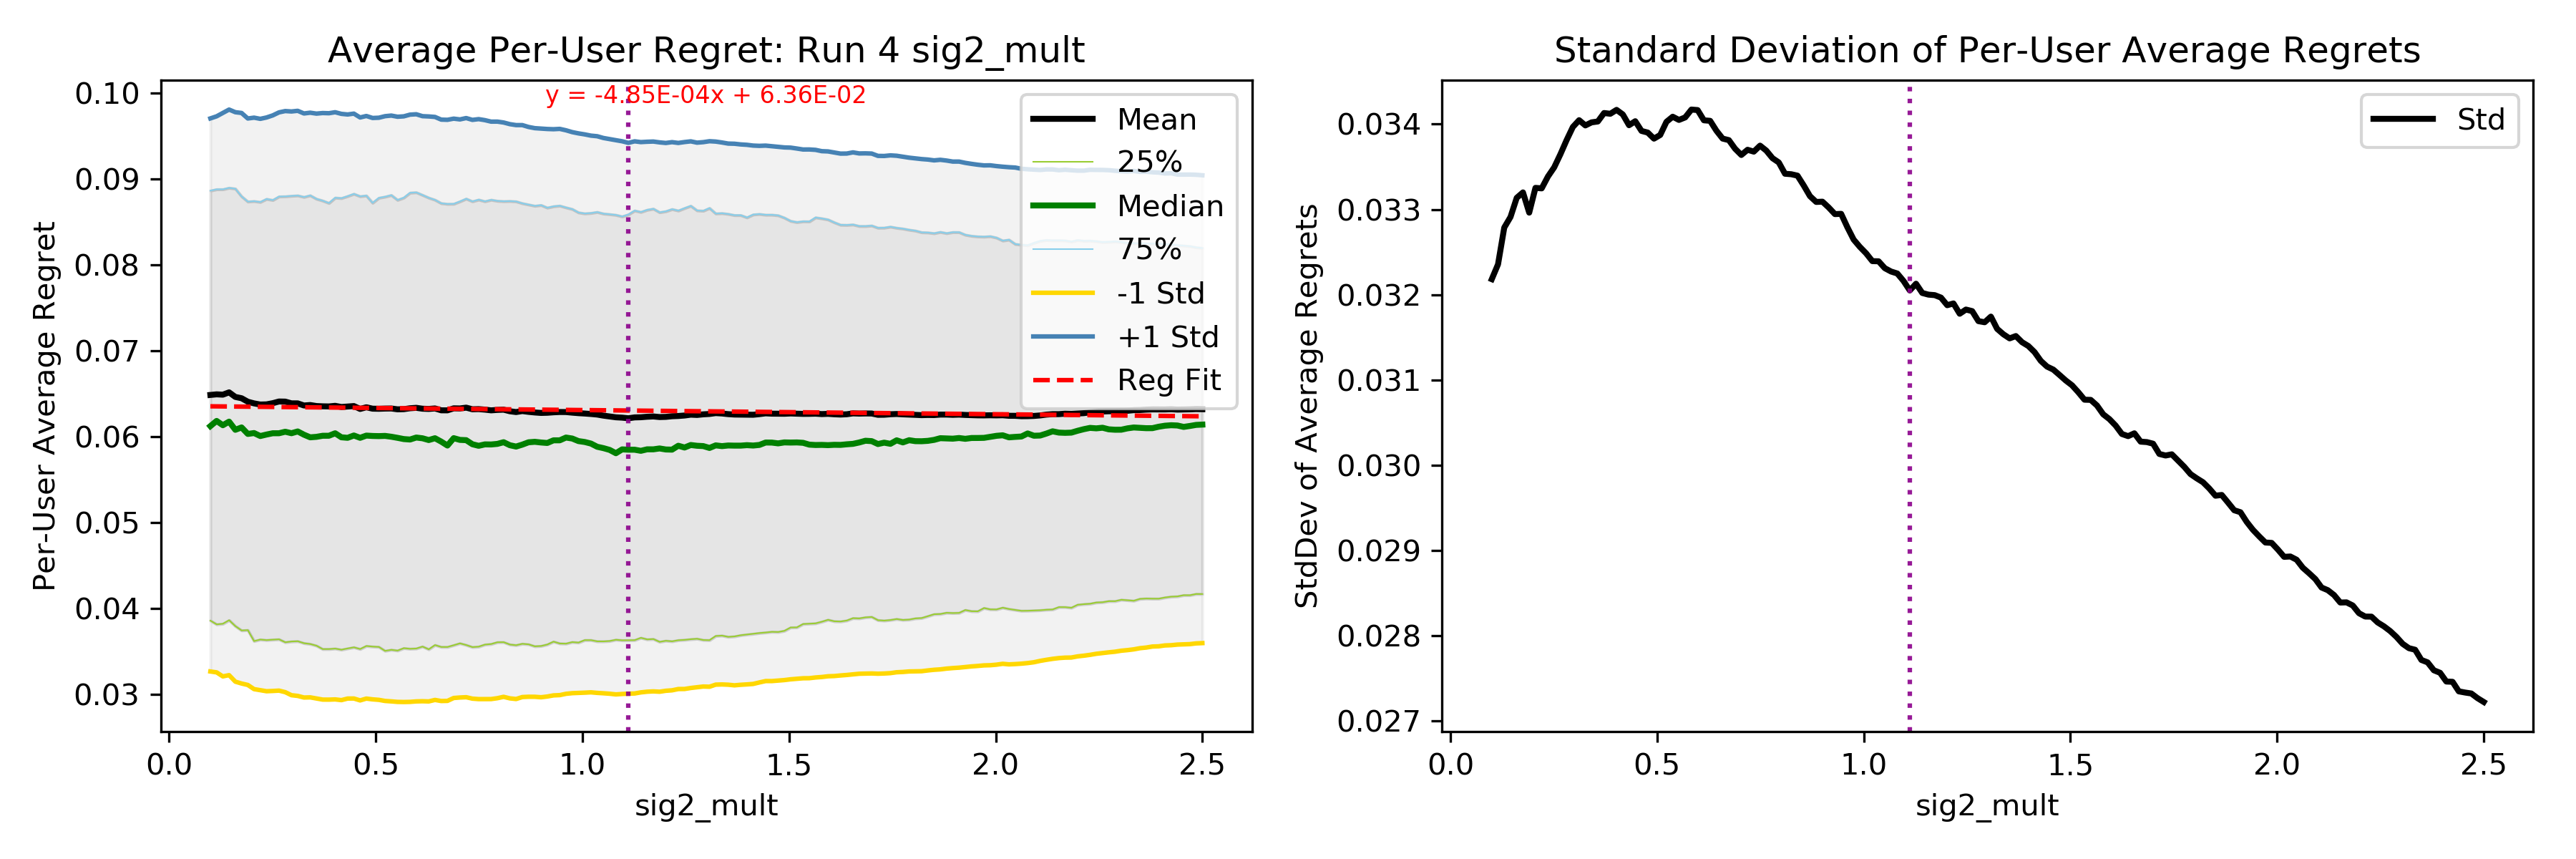
\includegraphics[width=1.1\textwidth,center]{figures/opt_param/opt_param_11100_sig2_mult4.png}%
	\caption{$MUER$ for Varying $\mathtt{sig2\_mult}$, $MUER$ Minimization Optimization}
	\end{figure}

	\begin{figure}[H]
	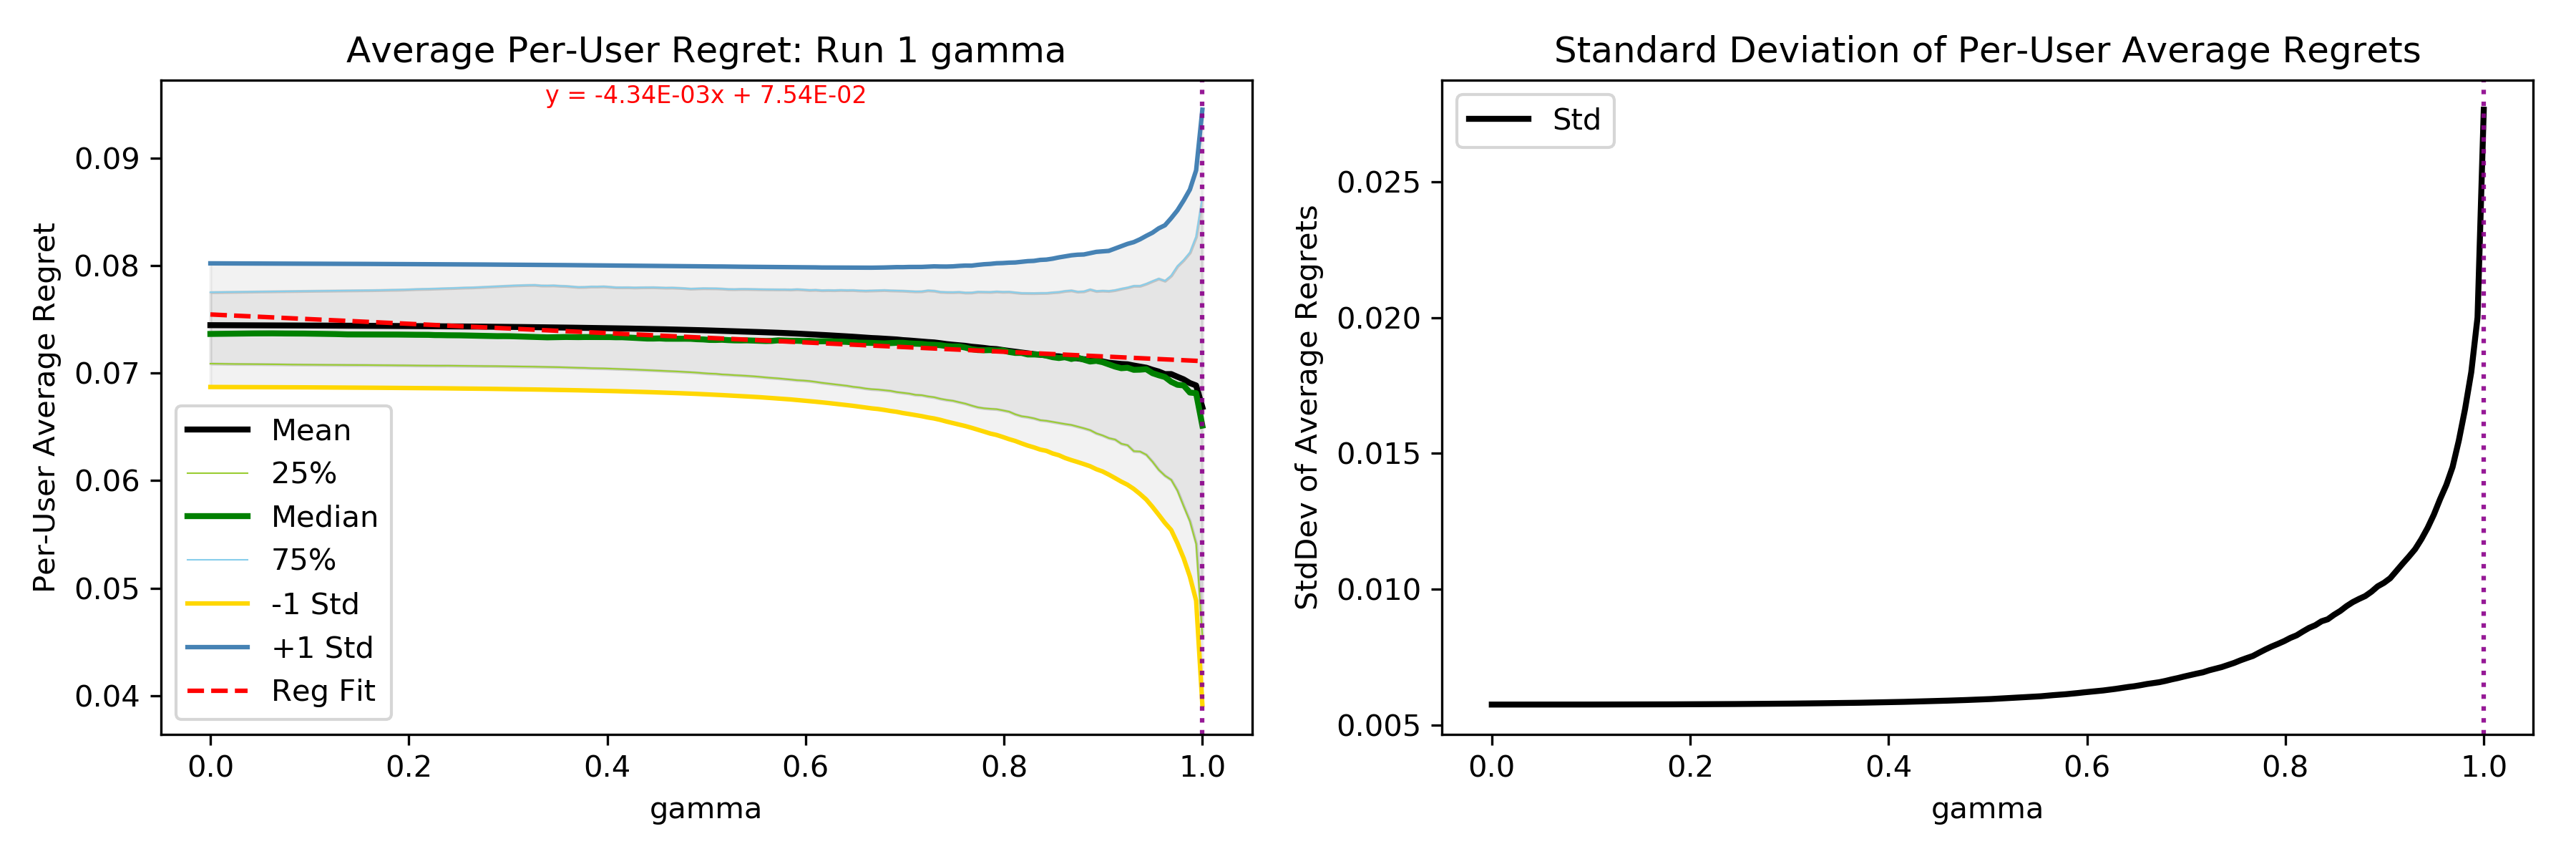
\includegraphics[width=1.1\textwidth,center]{figures/opt_param/opt_param_11100_gamma1.png}%
	\newline
	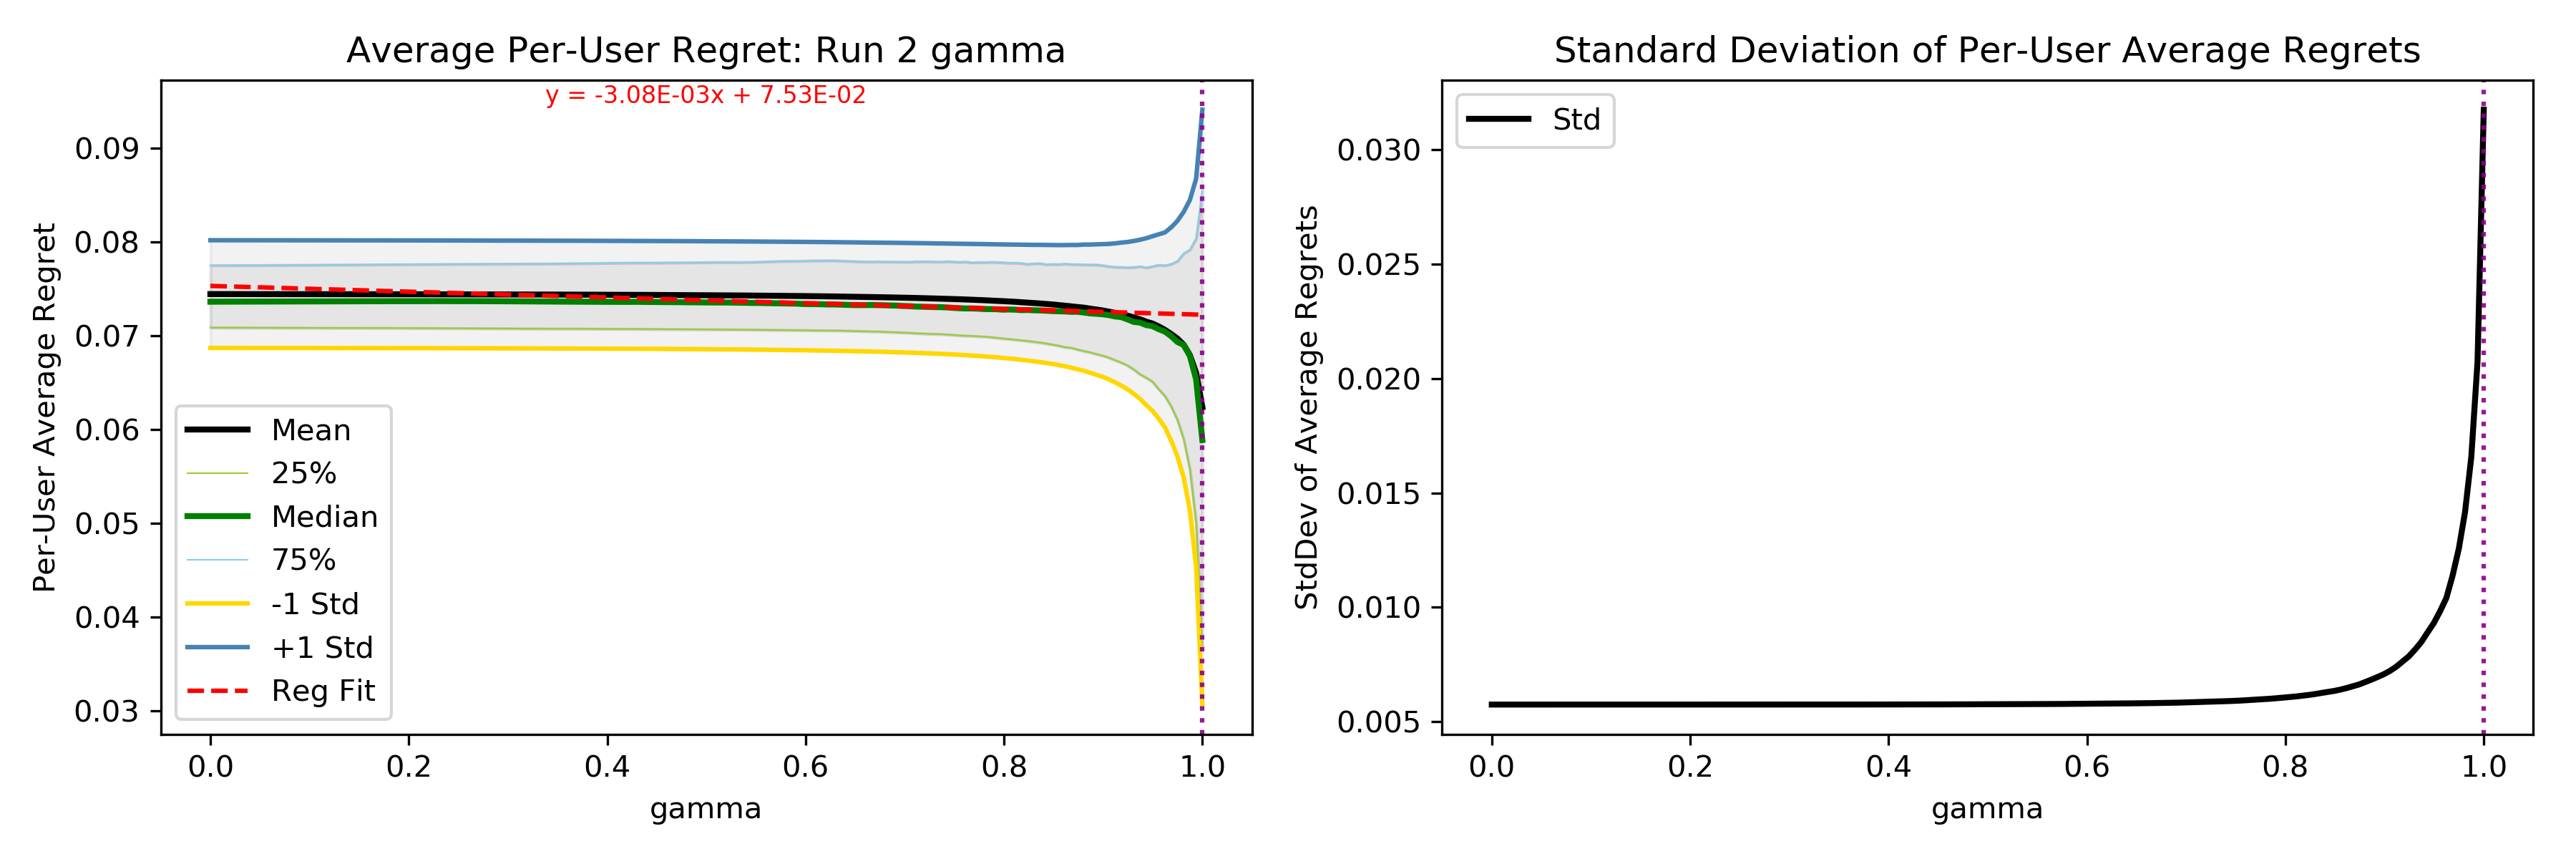
\includegraphics[width=1.1\textwidth,center]{figures/opt_param/opt_param_11100_gamma2.png}%
	\newline
	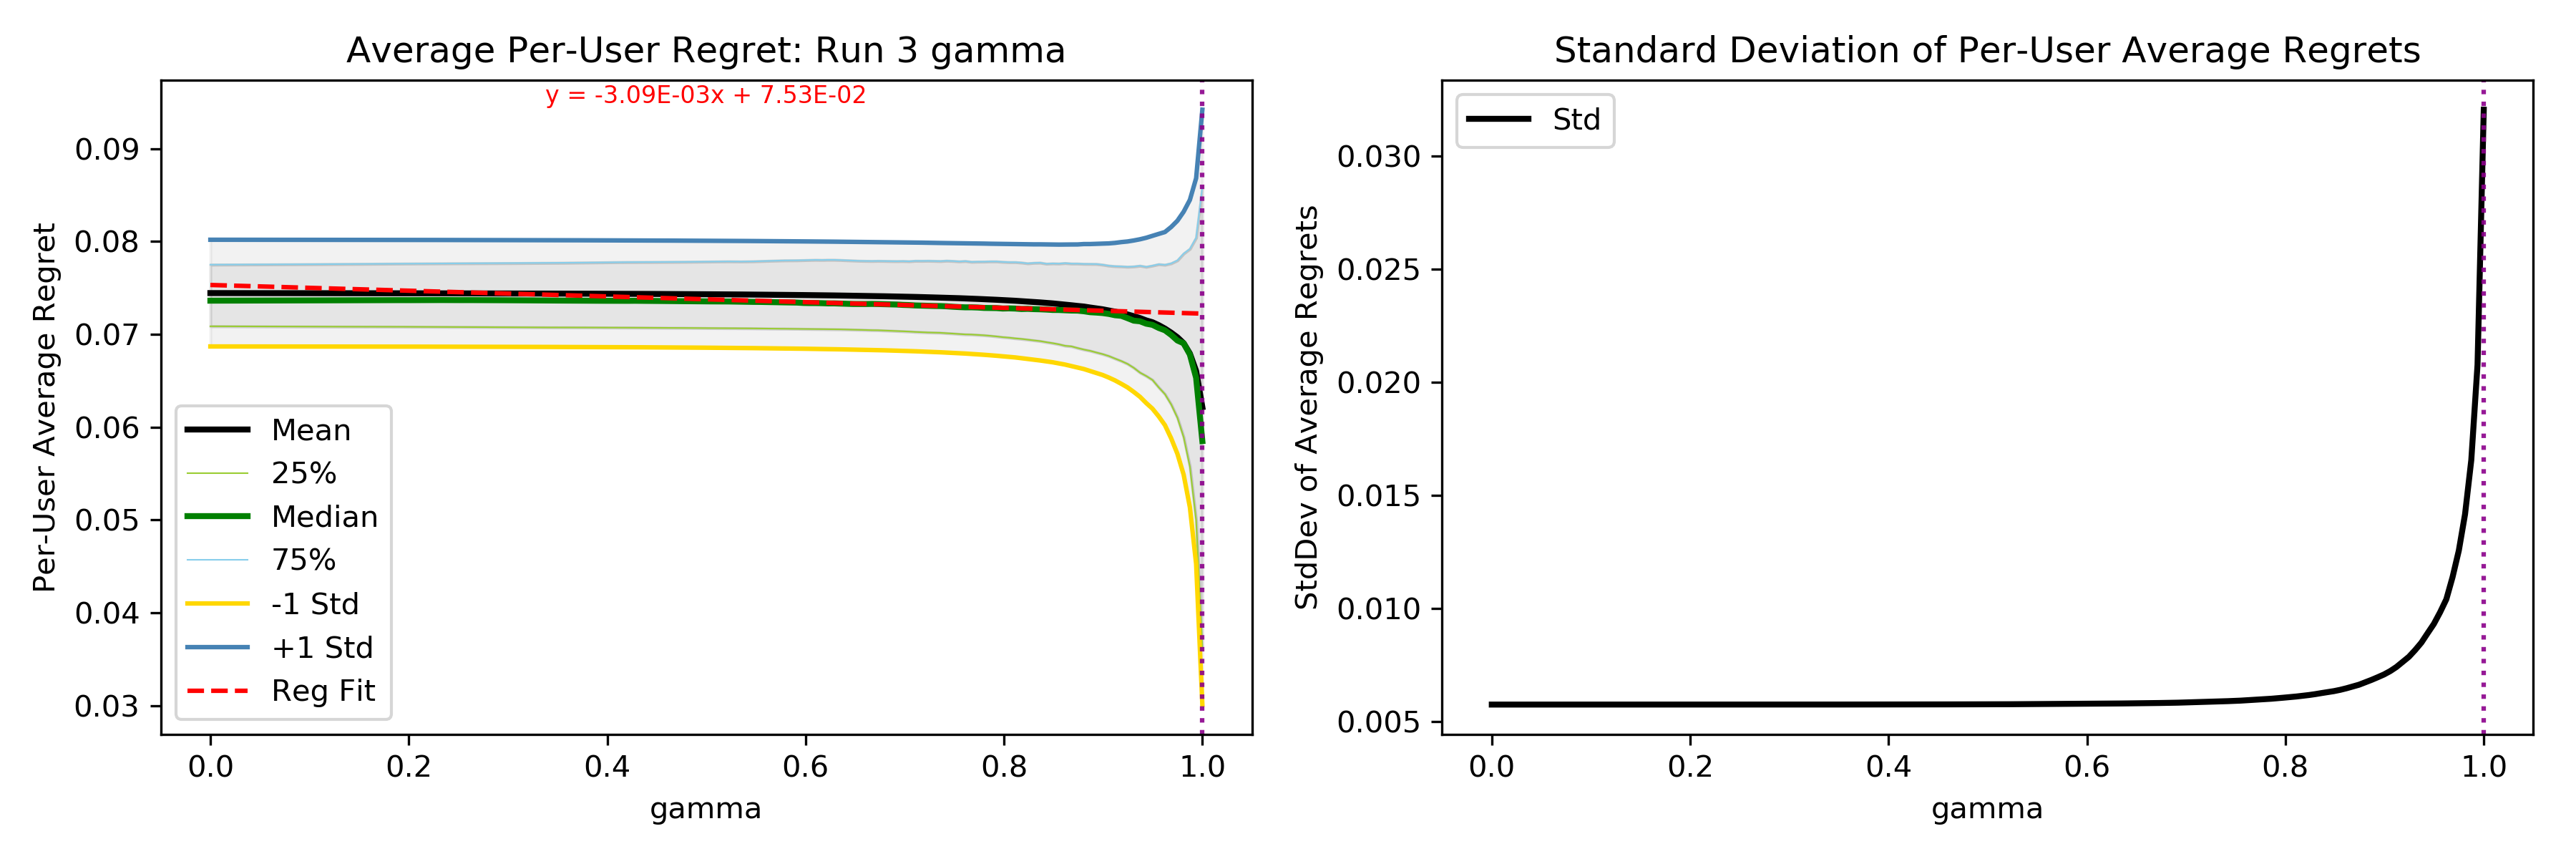
\includegraphics[width=1.1\textwidth,center]{figures/opt_param/opt_param_11100_gamma3.png}%
	\newline
	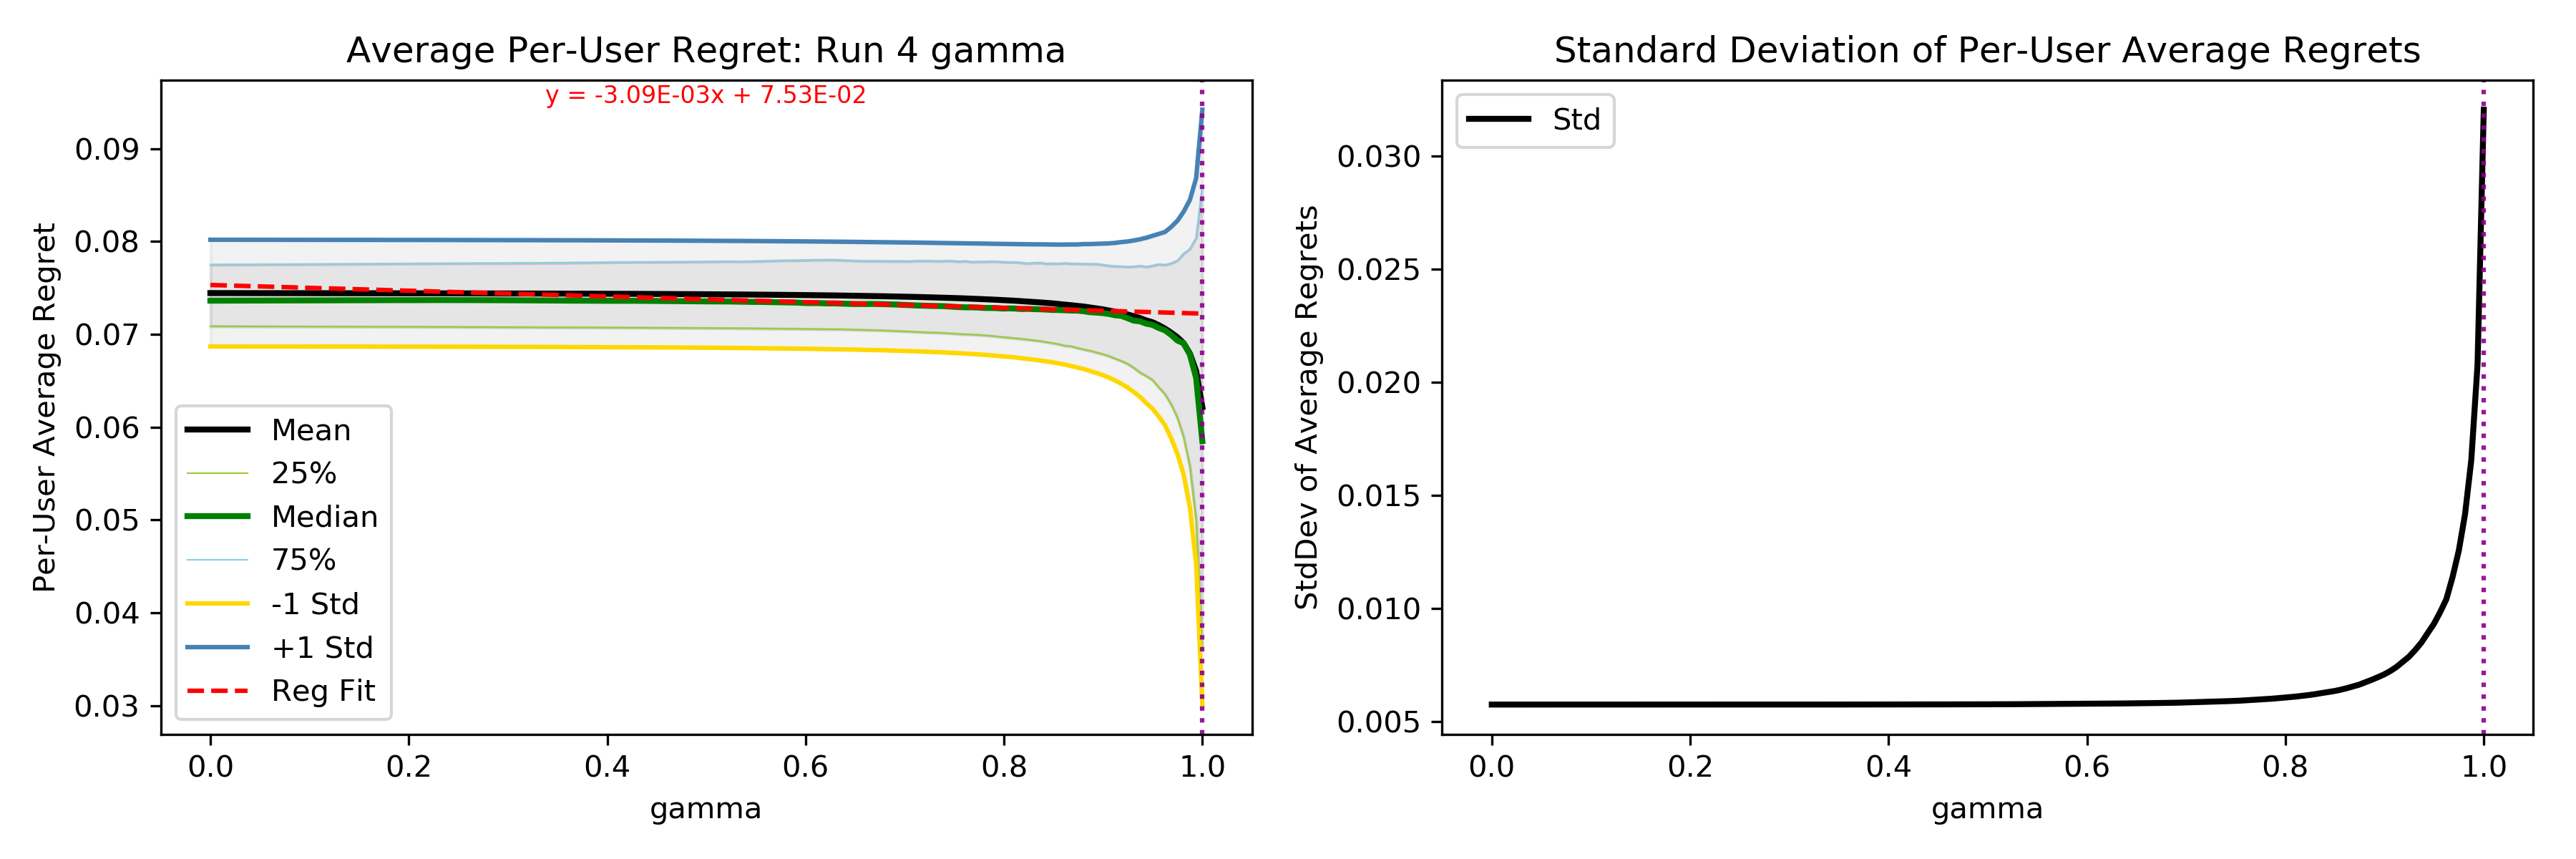
\includegraphics[width=1.1\textwidth,center]{figures/opt_param/opt_param_11100_gamma4.png}%
	\caption{$MUER$ for Varying $\mathtt{gamma}$, $MUER$ Minimization Optimization}
	\end{figure}

	\begin{figure}[H]
	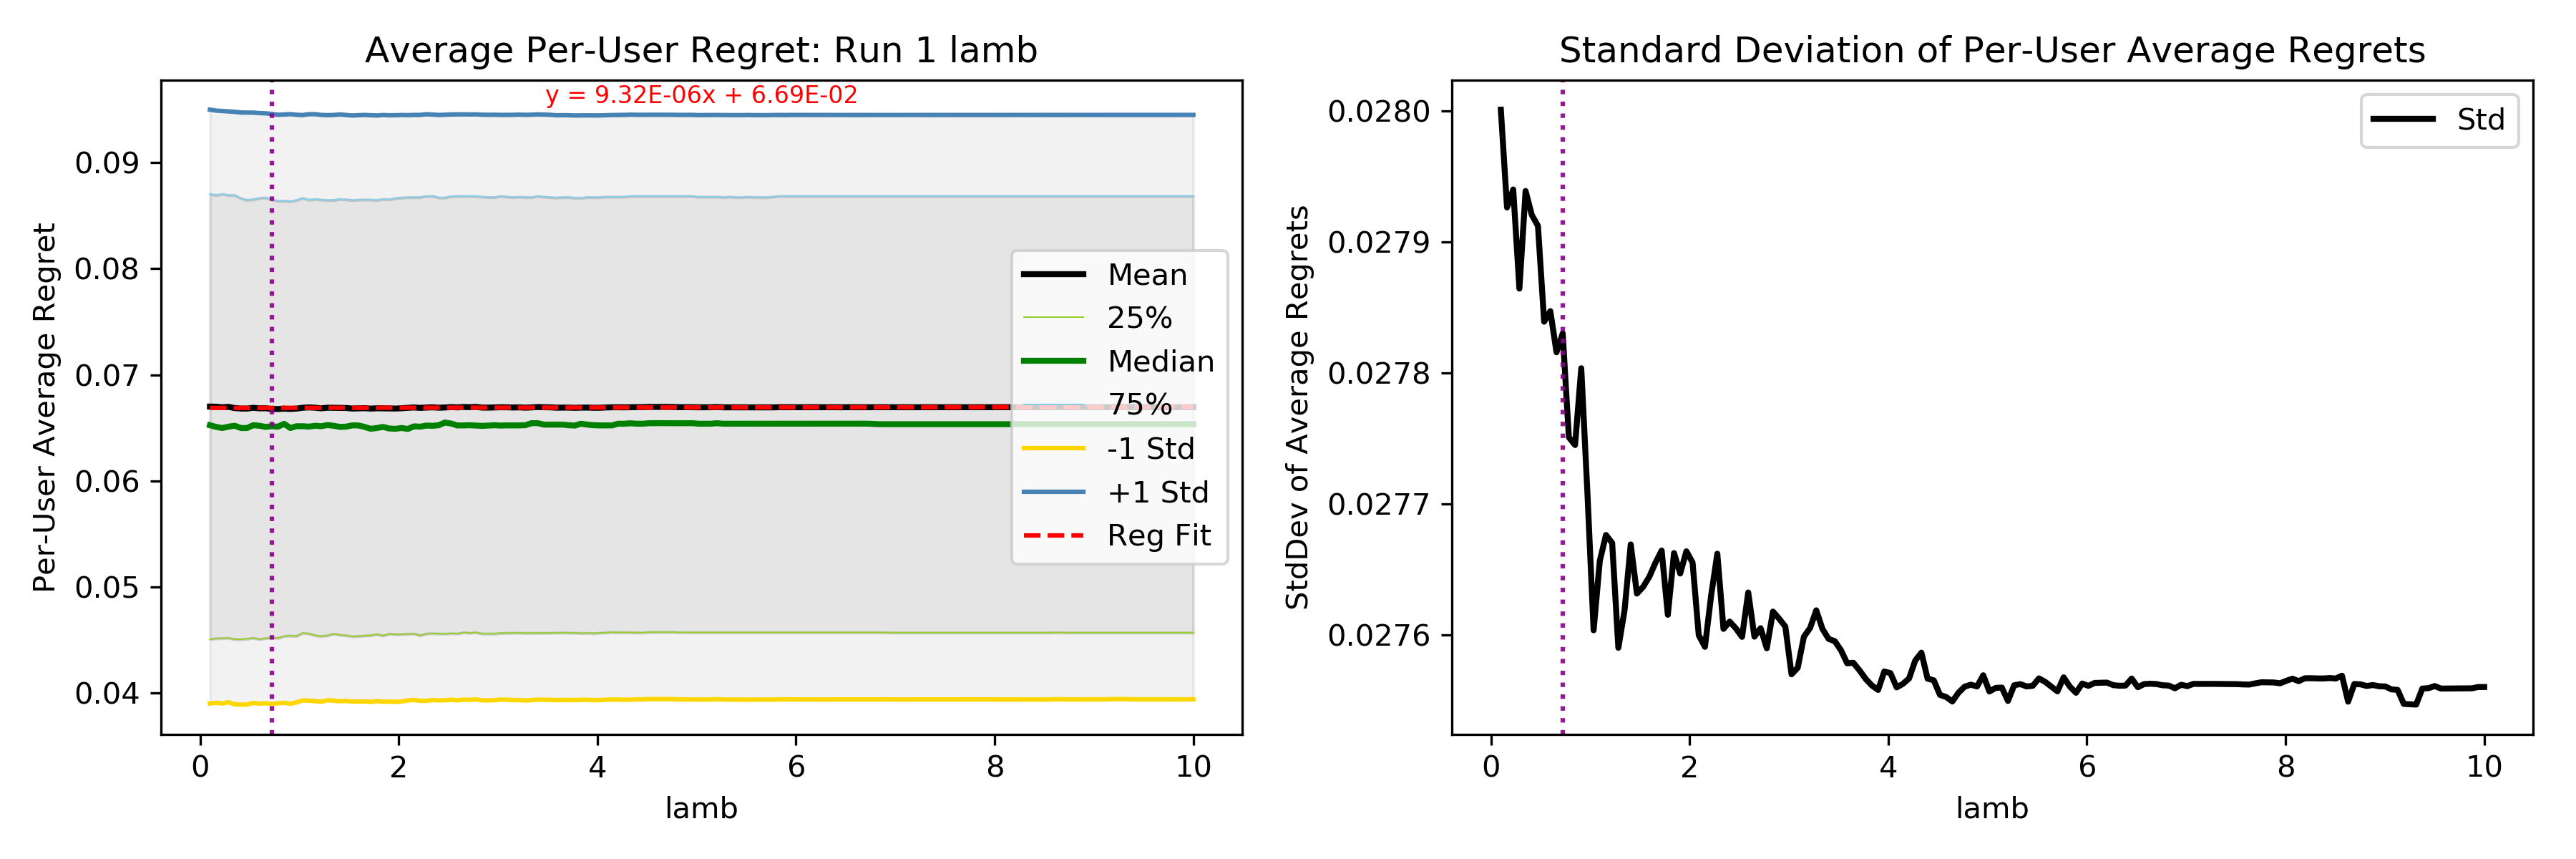
\includegraphics[width=1.1\textwidth,center]{figures/opt_param/opt_param_11100_lamb1.png}%
	\newline
	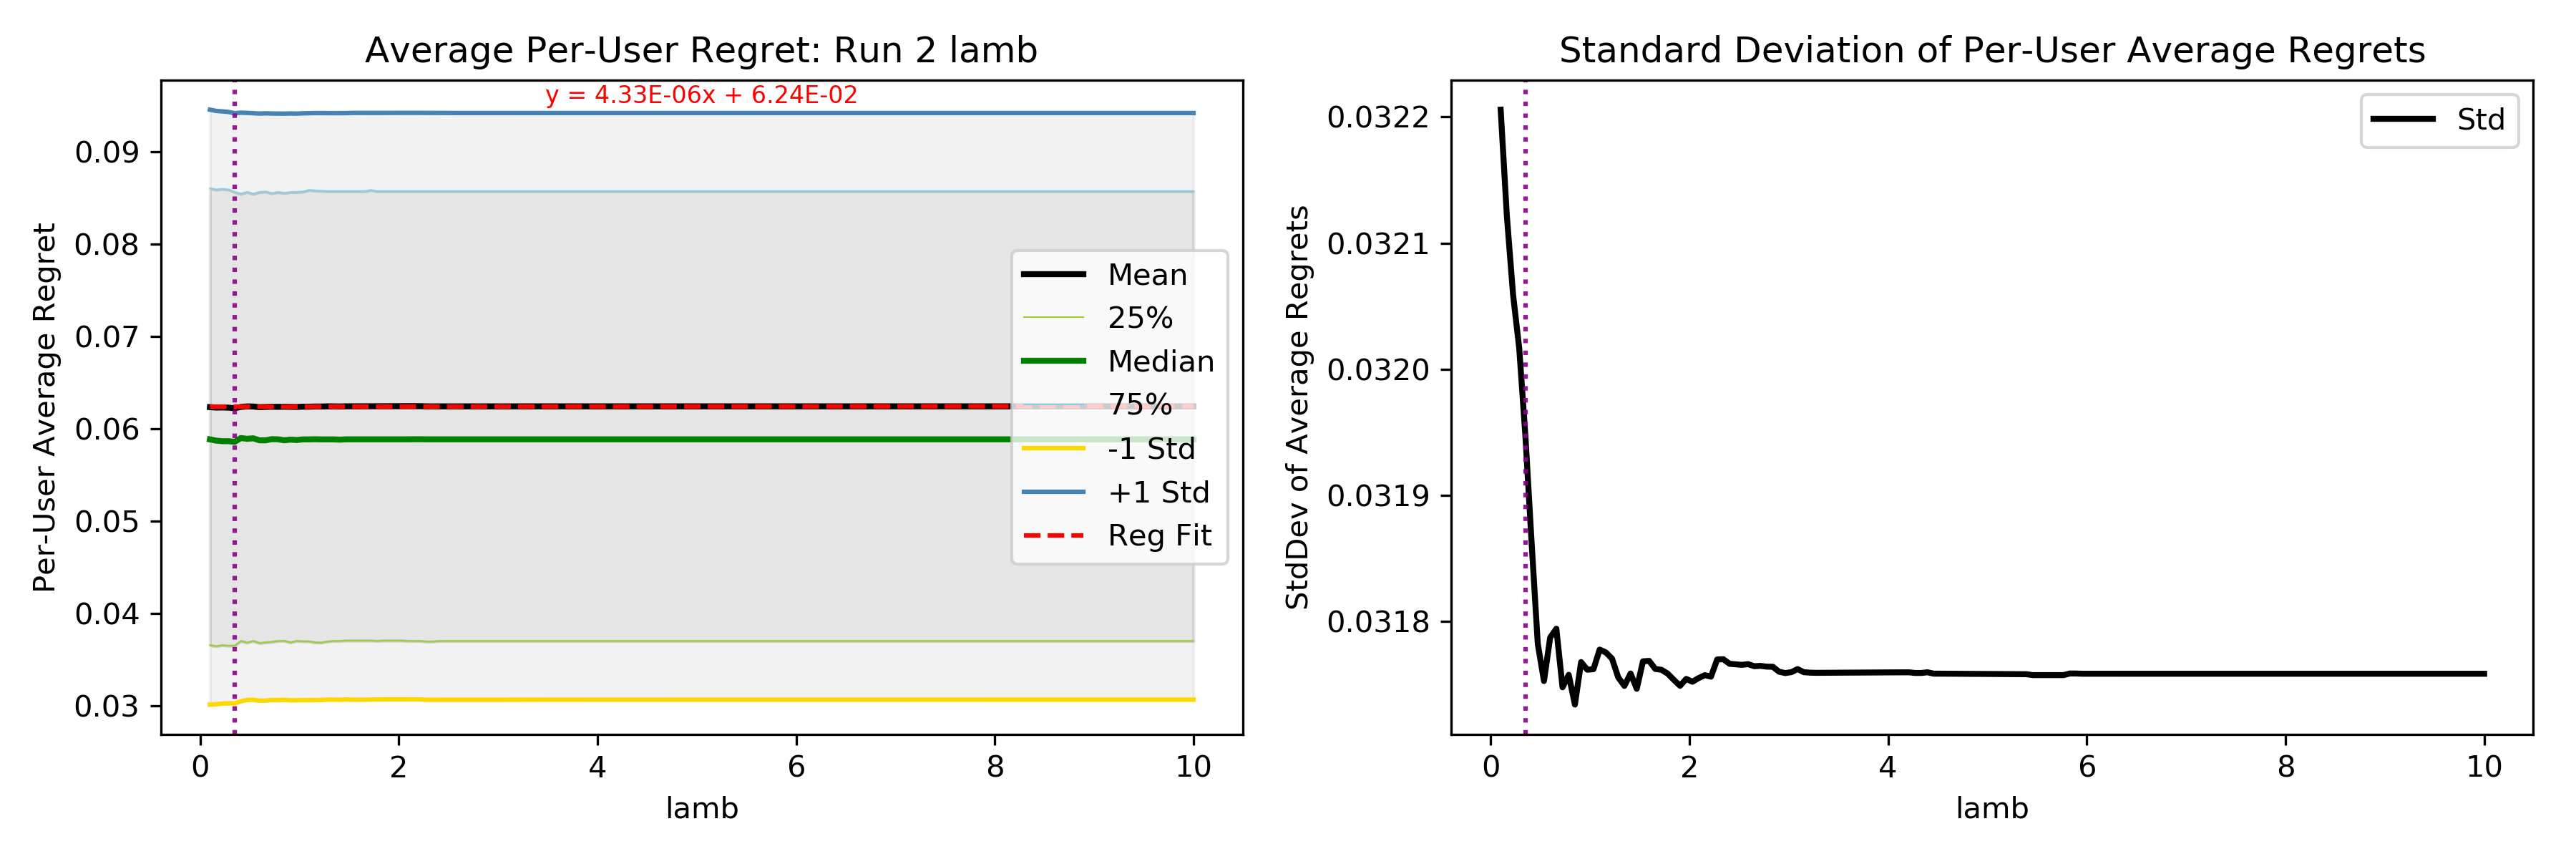
\includegraphics[width=1.1\textwidth,center]{figures/opt_param/opt_param_11100_lamb2.png}%
	\newline
	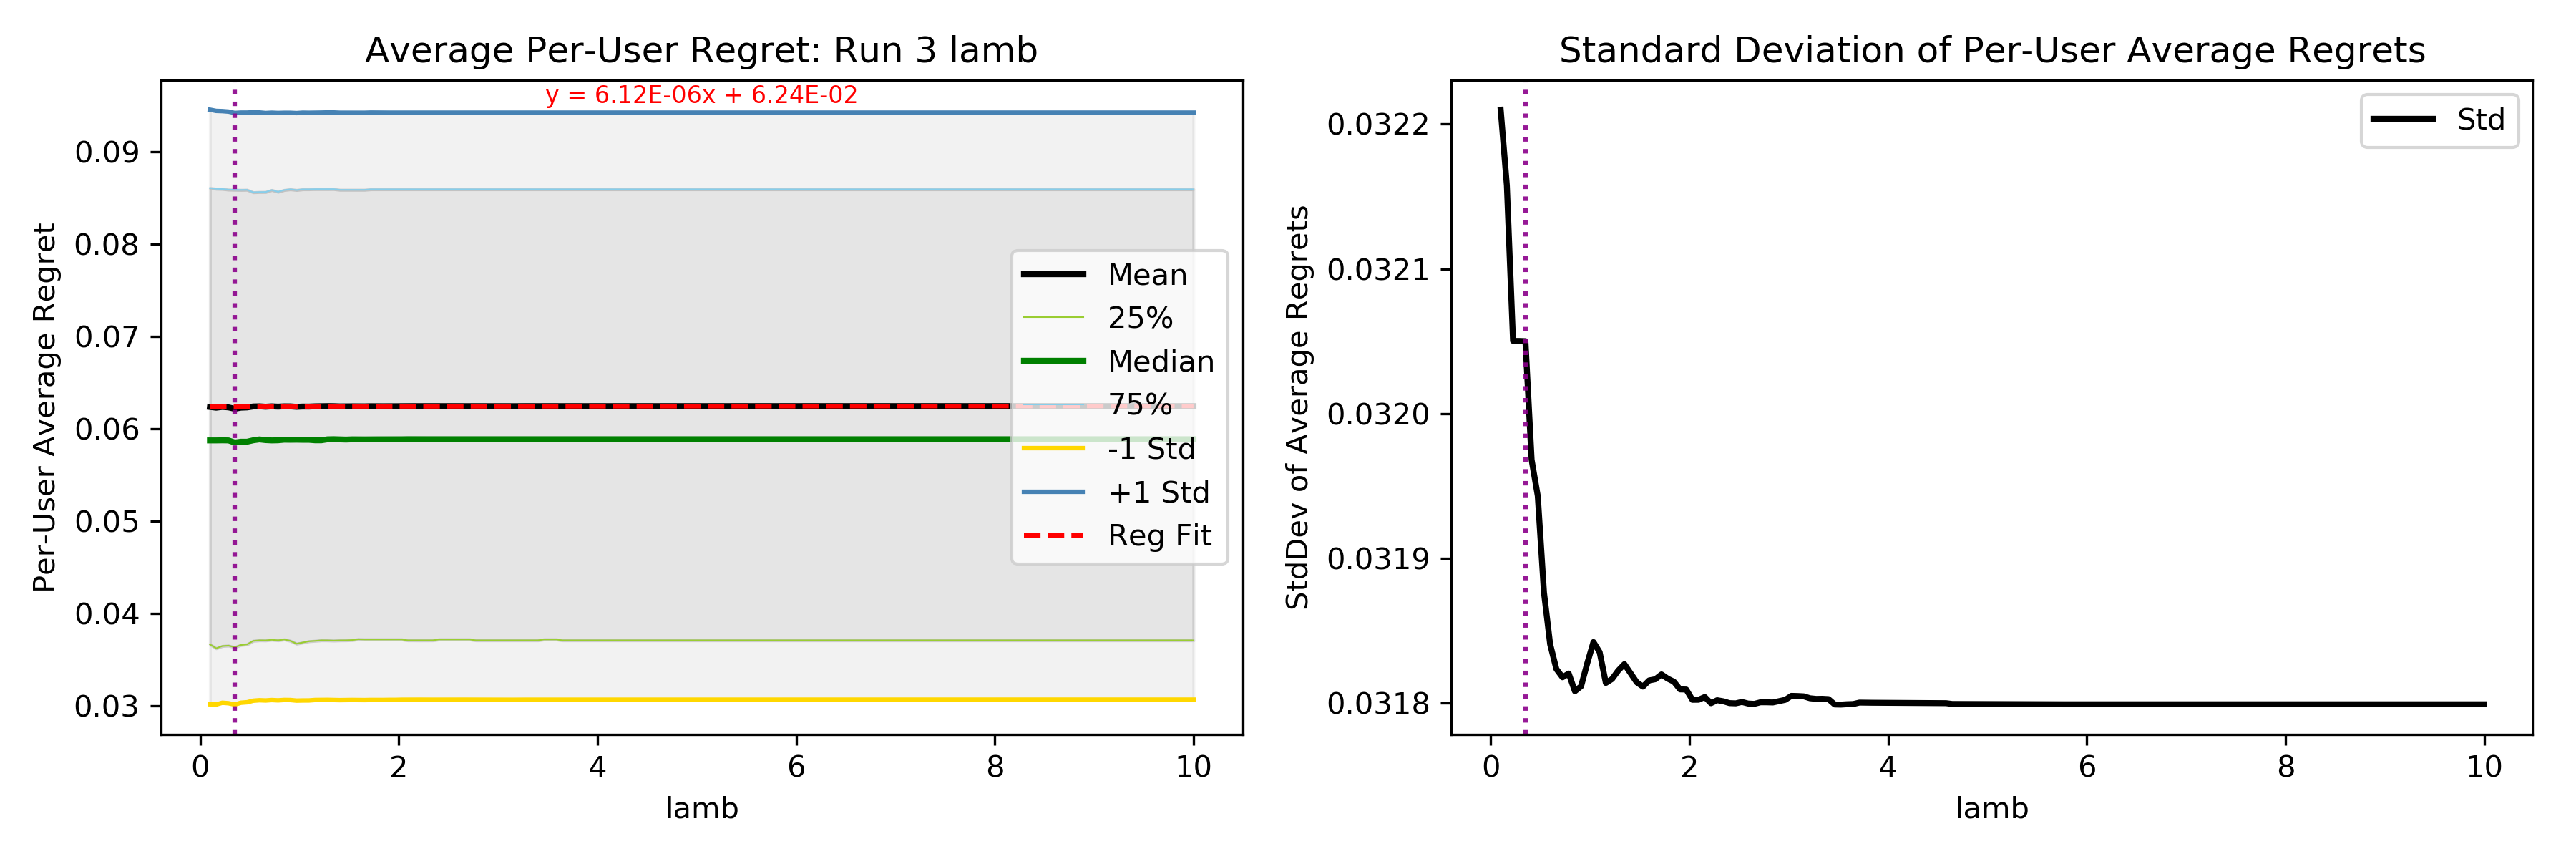
\includegraphics[width=1.1\textwidth,center]{figures/opt_param/opt_param_11100_lamb3.png}%
	\newline
	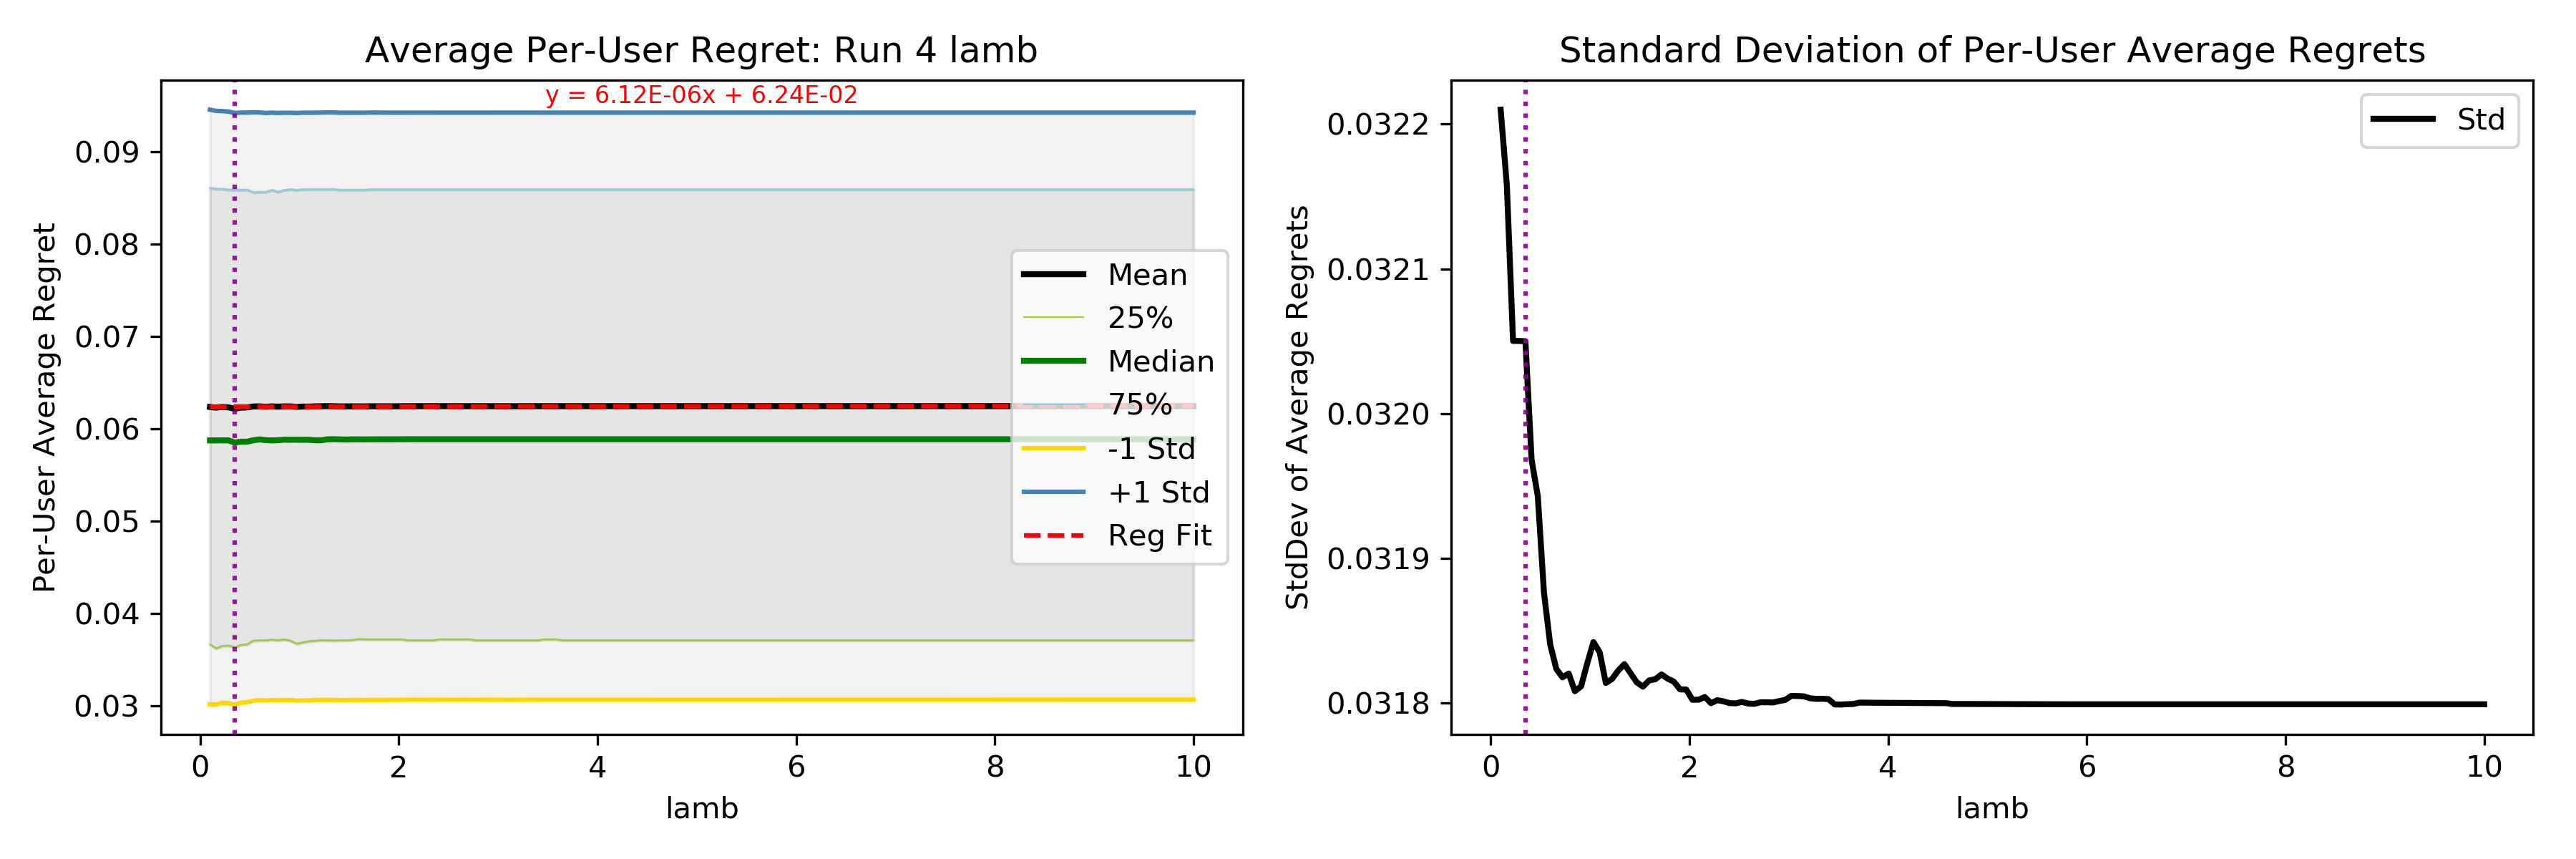
\includegraphics[width=1.1\textwidth,center]{figures/opt_param/opt_param_11100_lamb4.png}%
	\caption{$MUER$ for Varying $\mathtt{lamb}$, $MUER$ Minimization Optimization}
	\end{figure}

	\begin{figure}[H]
	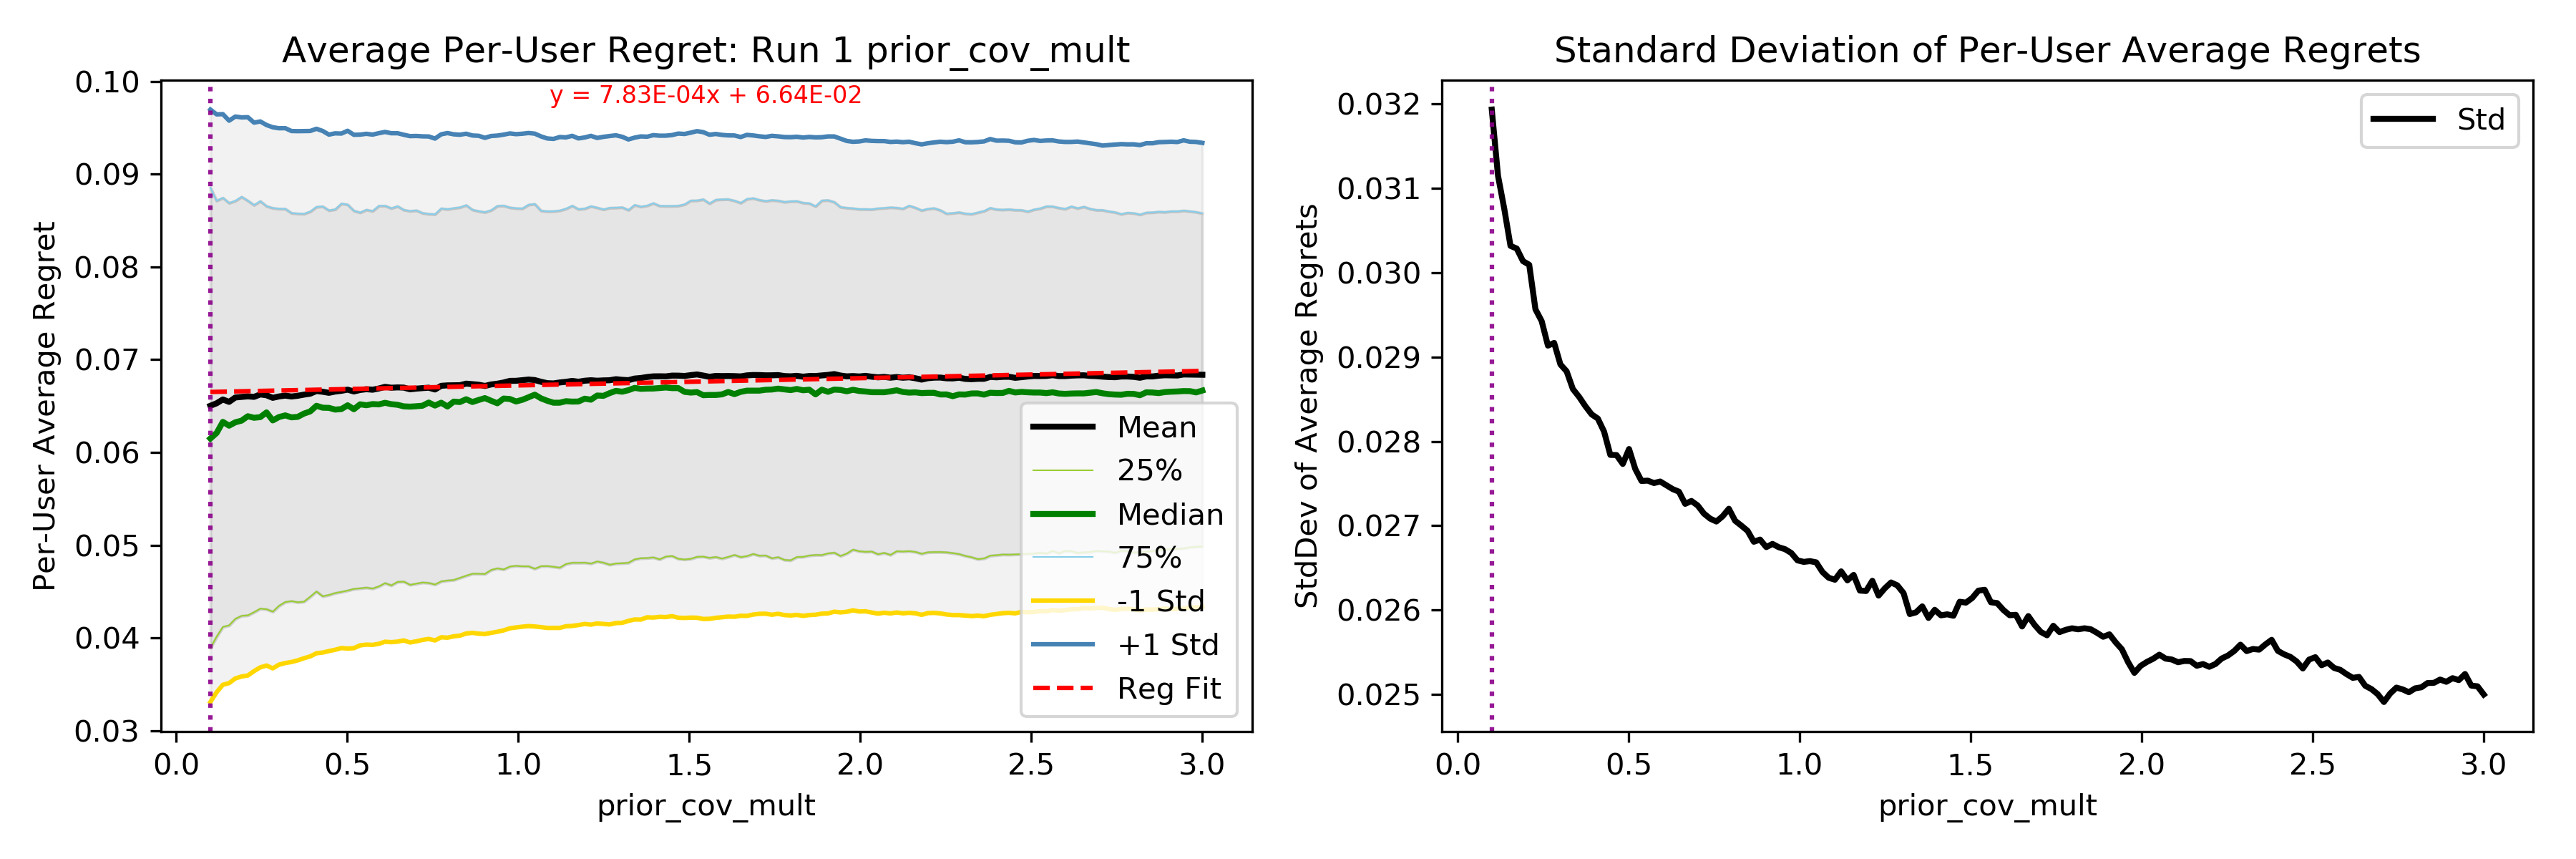
\includegraphics[width=1.1\textwidth,center]{figures/opt_param/opt_param_11100_prior_cov_mult1.png}%
	\newline
	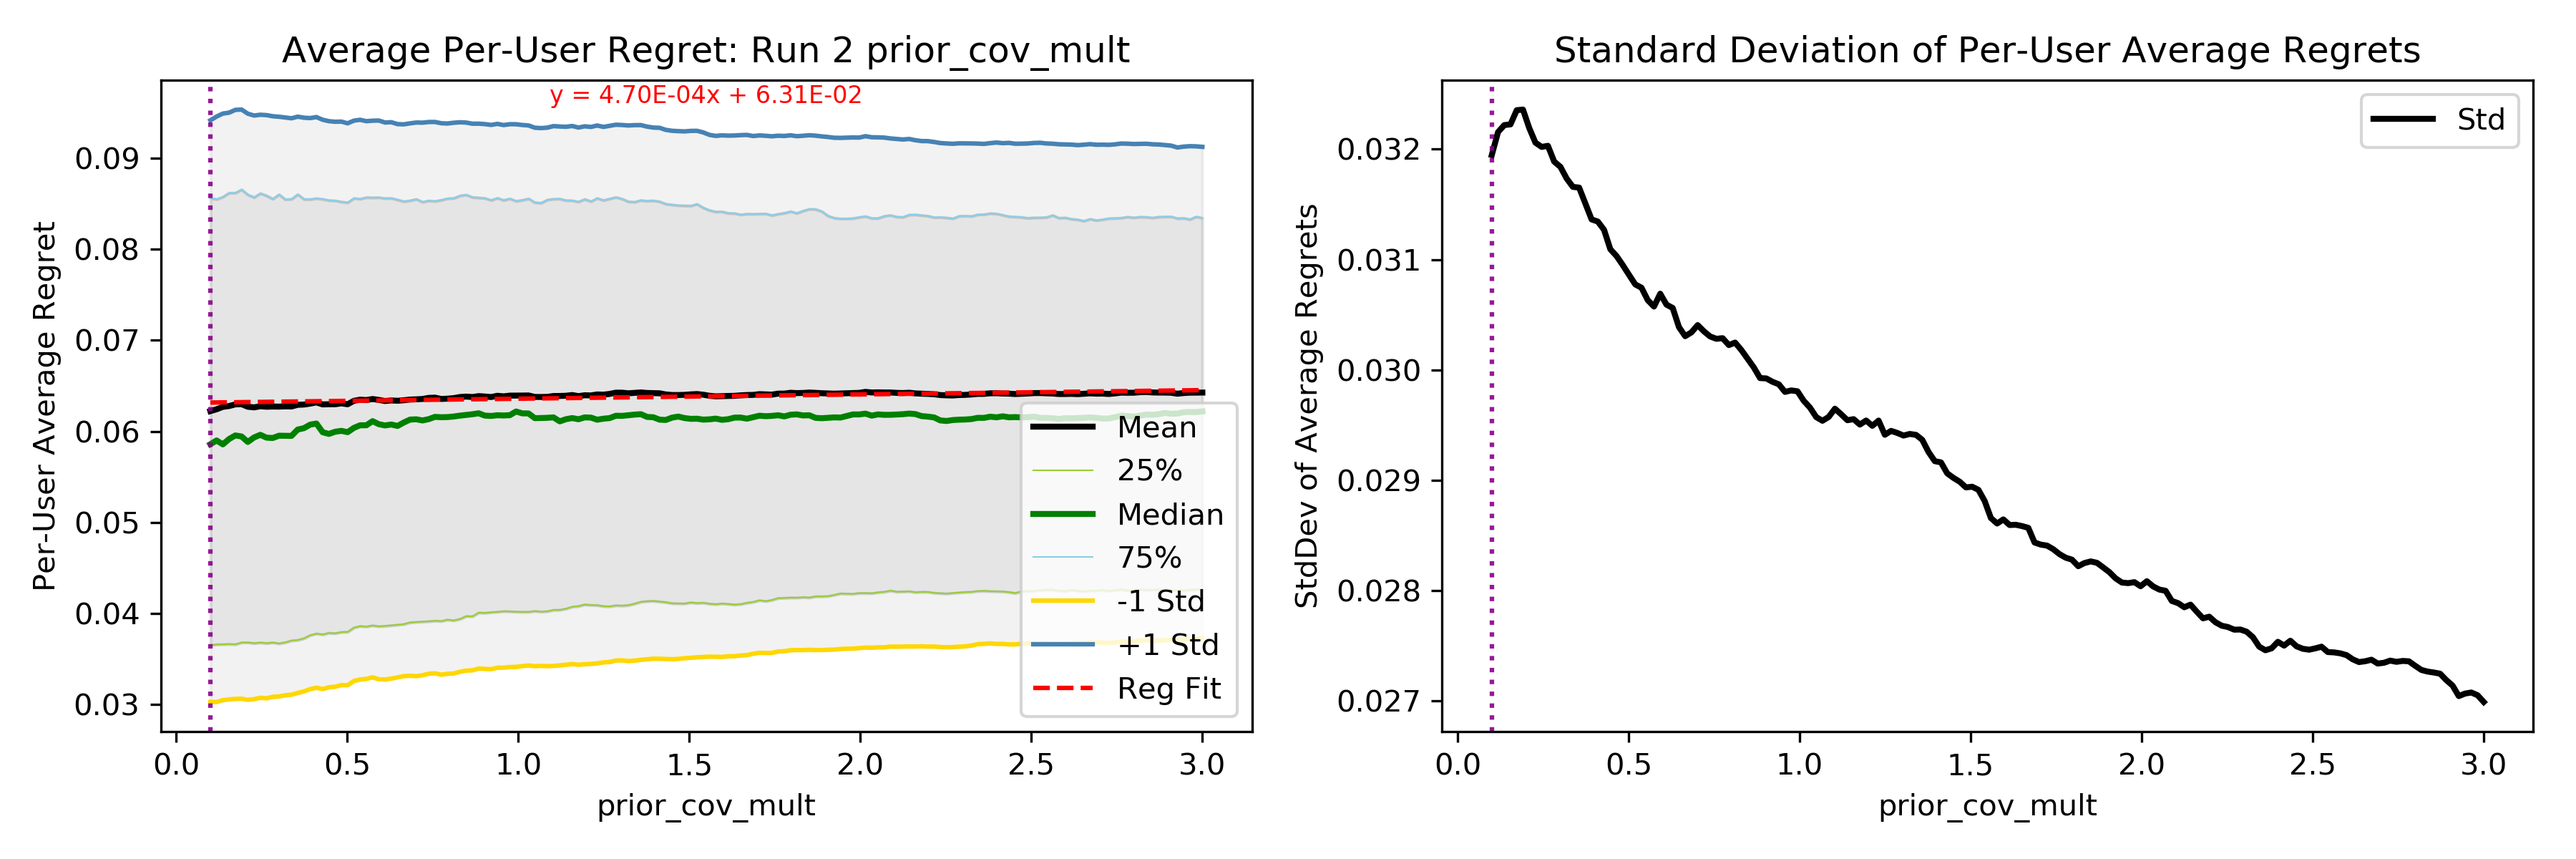
\includegraphics[width=1.1\textwidth,center]{figures/opt_param/opt_param_11100_prior_cov_mult2.png}%
	\newline
	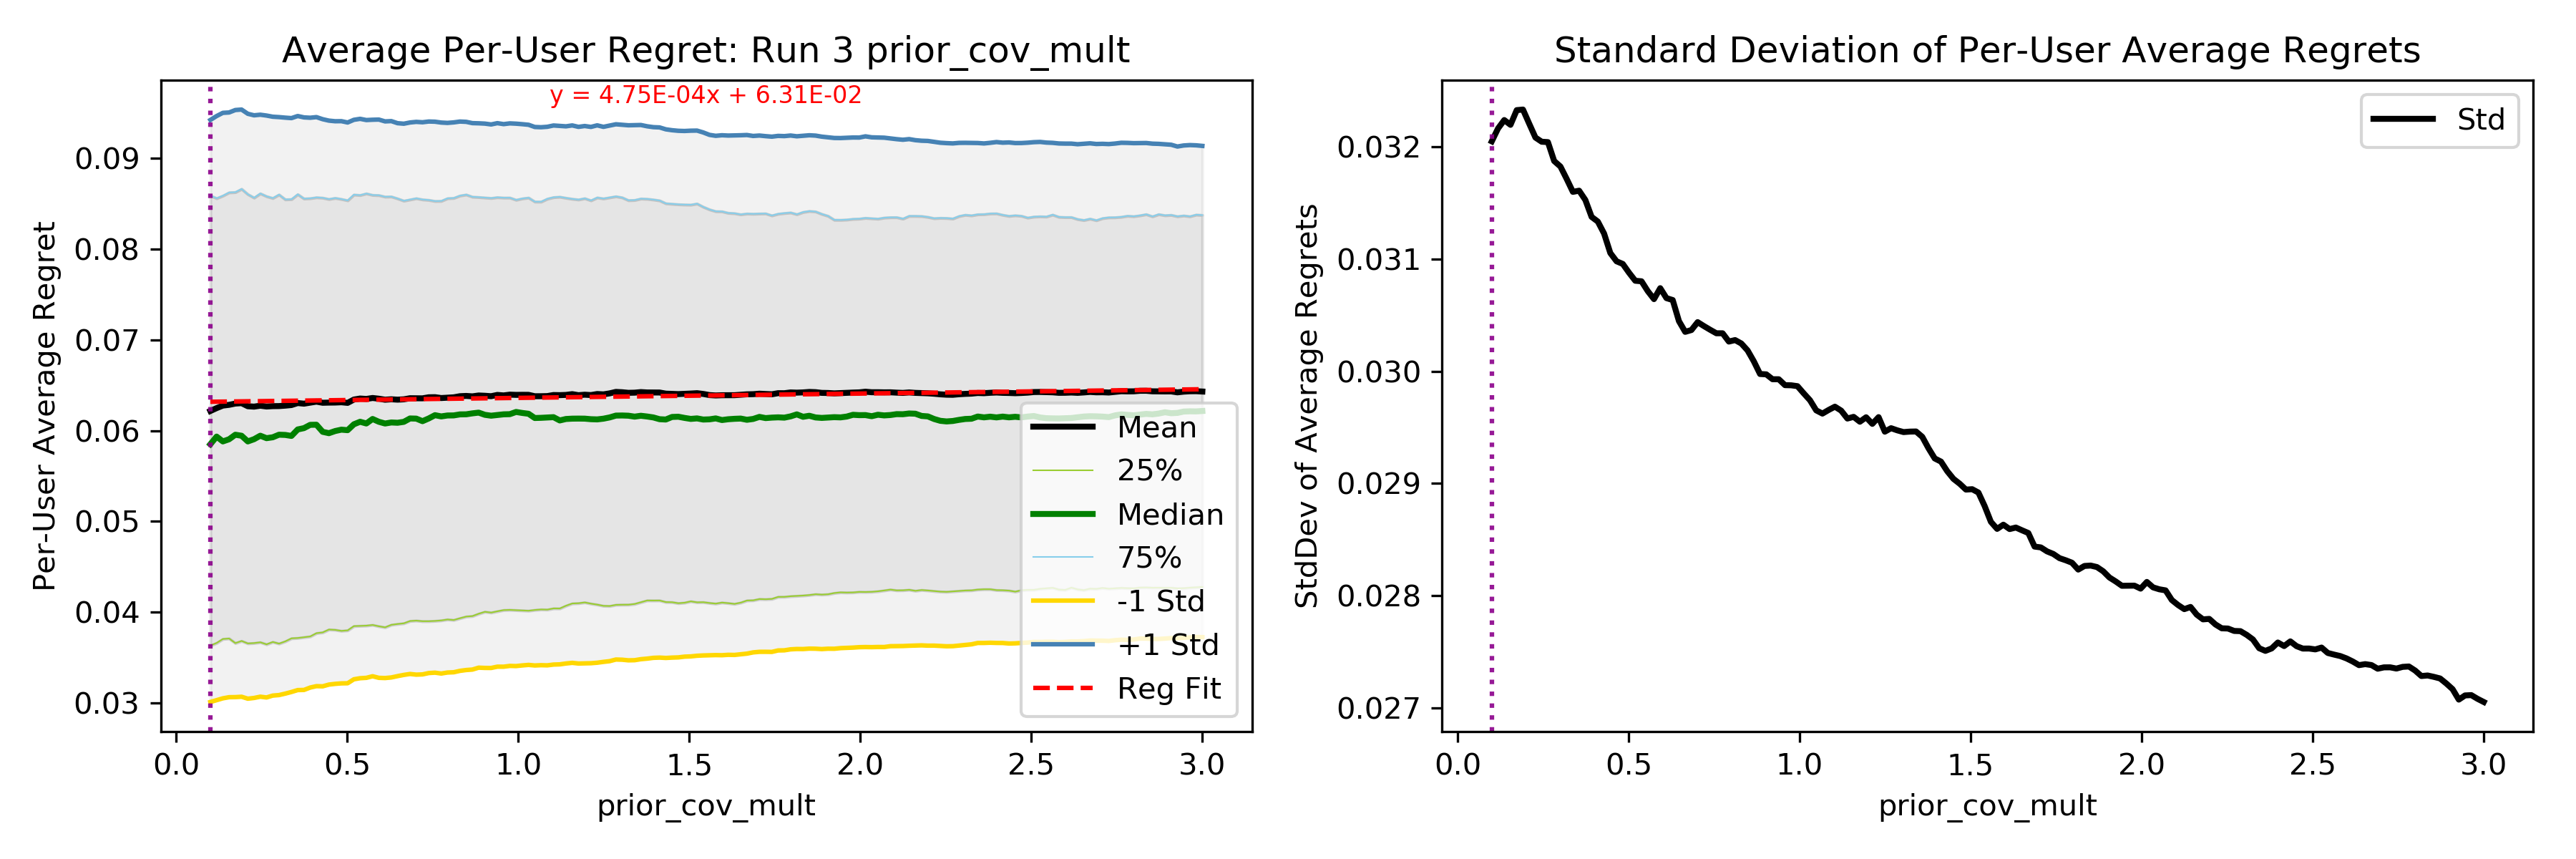
\includegraphics[width=1.1\textwidth,center]{figures/opt_param/opt_param_11100_prior_cov_mult3.png}%
	\newline
	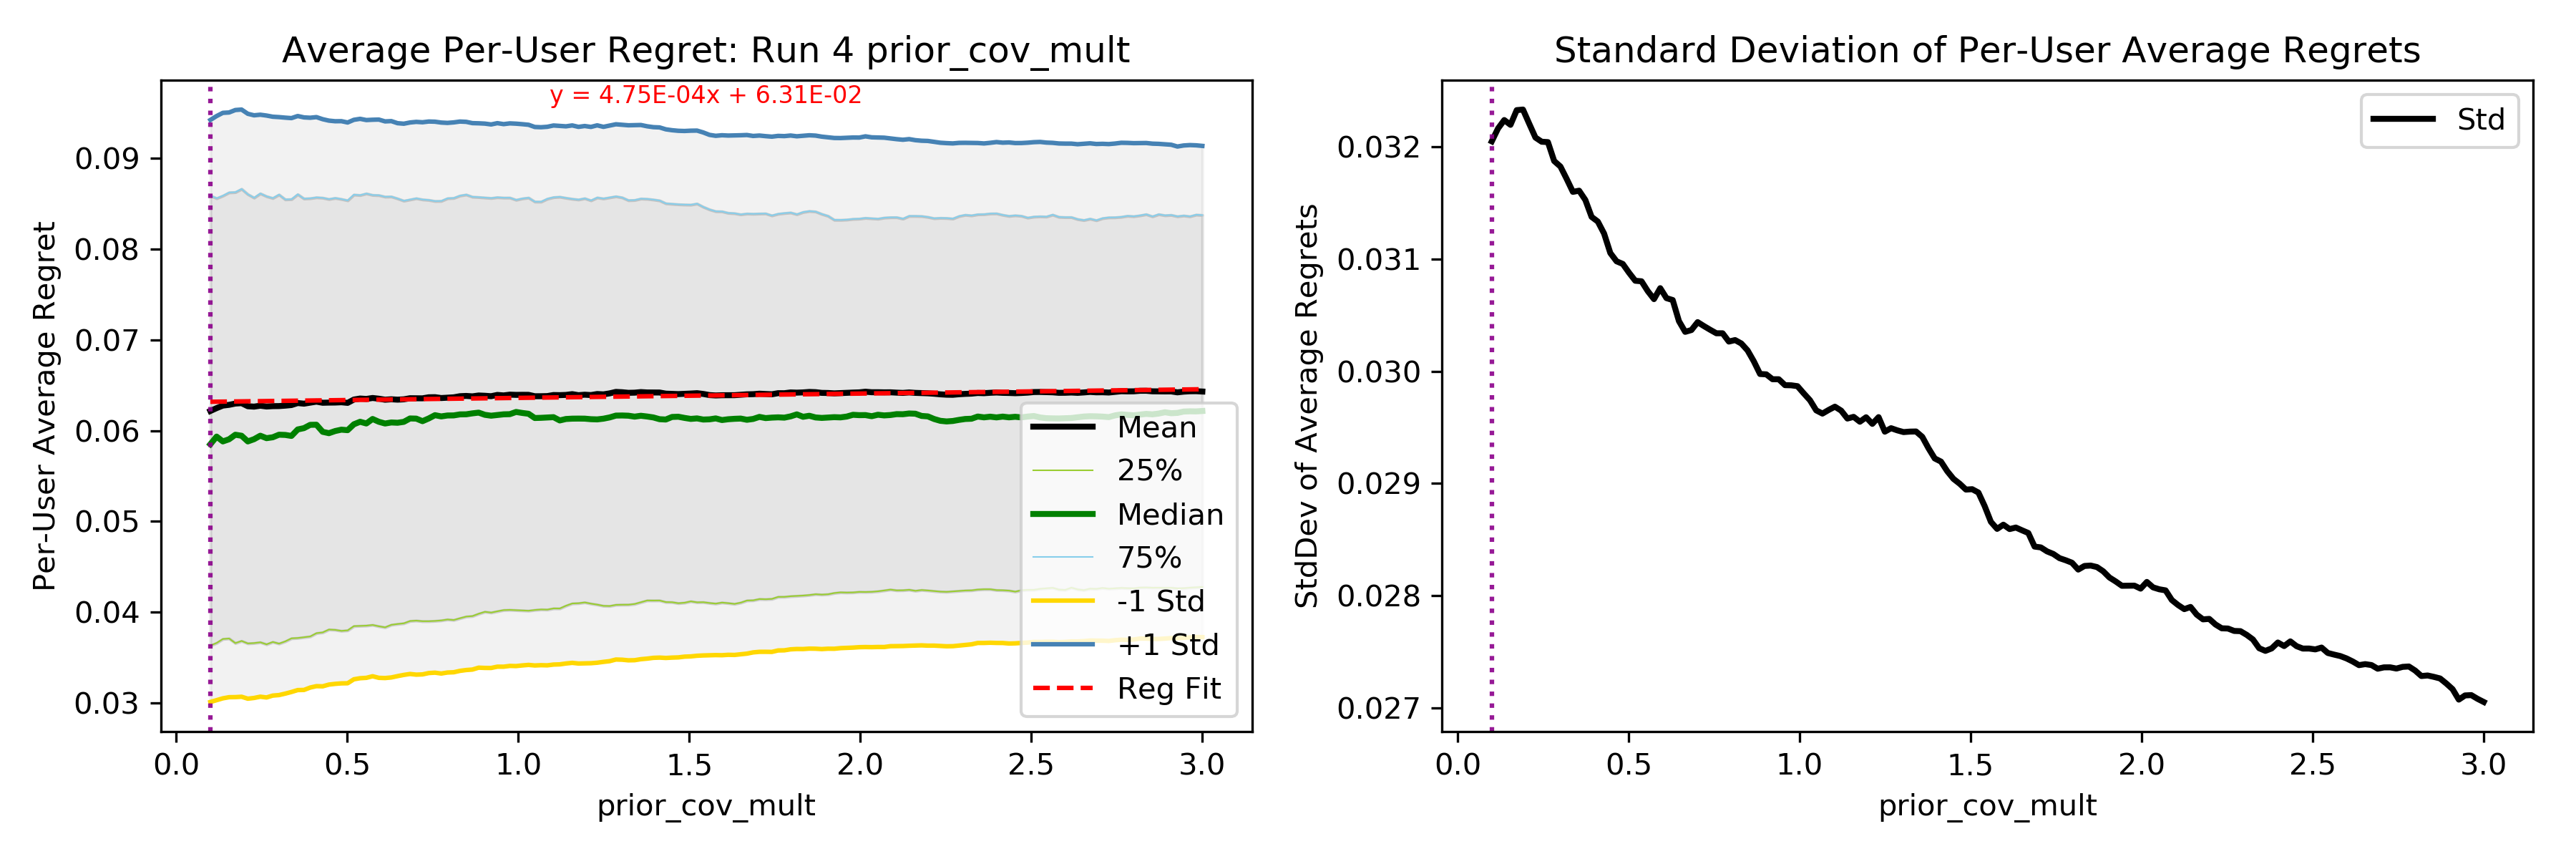
\includegraphics[width=1.1\textwidth,center]{figures/opt_param/opt_param_11100_prior_cov_mult4.png}%
	\caption{$MUER$ for Varying $\mathtt{prior\_cov\_mult}$, $MUER$ Minimization Optimization}
	\end{figure}

	\fi
	%%%%%%%%%%%%%%%%%%%%%%%%%%%%%%%%%%%%%%%%%%%%%%%%%%%%%%%%%%%%%%%




% \subsection{Standard Deviation Cutoff Parameter Optimization}
% 	\label{Standard Deviation Cutoff Parameter Optimization}

	\ifdraft
	Turn off Draft mode to display figures!
	\else
	%%%%%%%%%%%%%%%%%%%%%%%%%%%%%%%%%%%%%%%%%%%%%%%%%%%%%%%%%%%%%%%%

	\begin{figure}[H]
	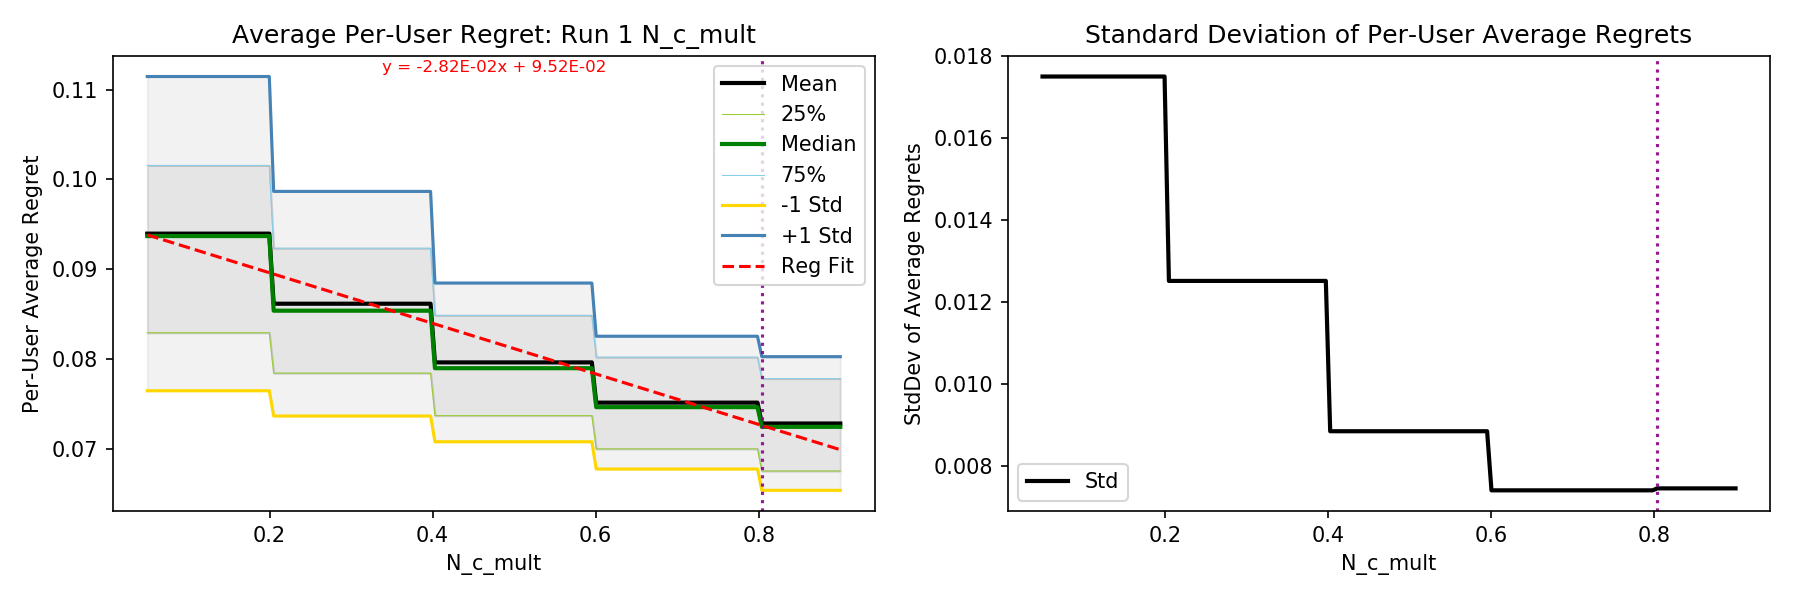
\includegraphics[width=1.1\textwidth,center]{figures/opt_param/opt_param_std_11100_N_c_mult1.png}%
	\newline
	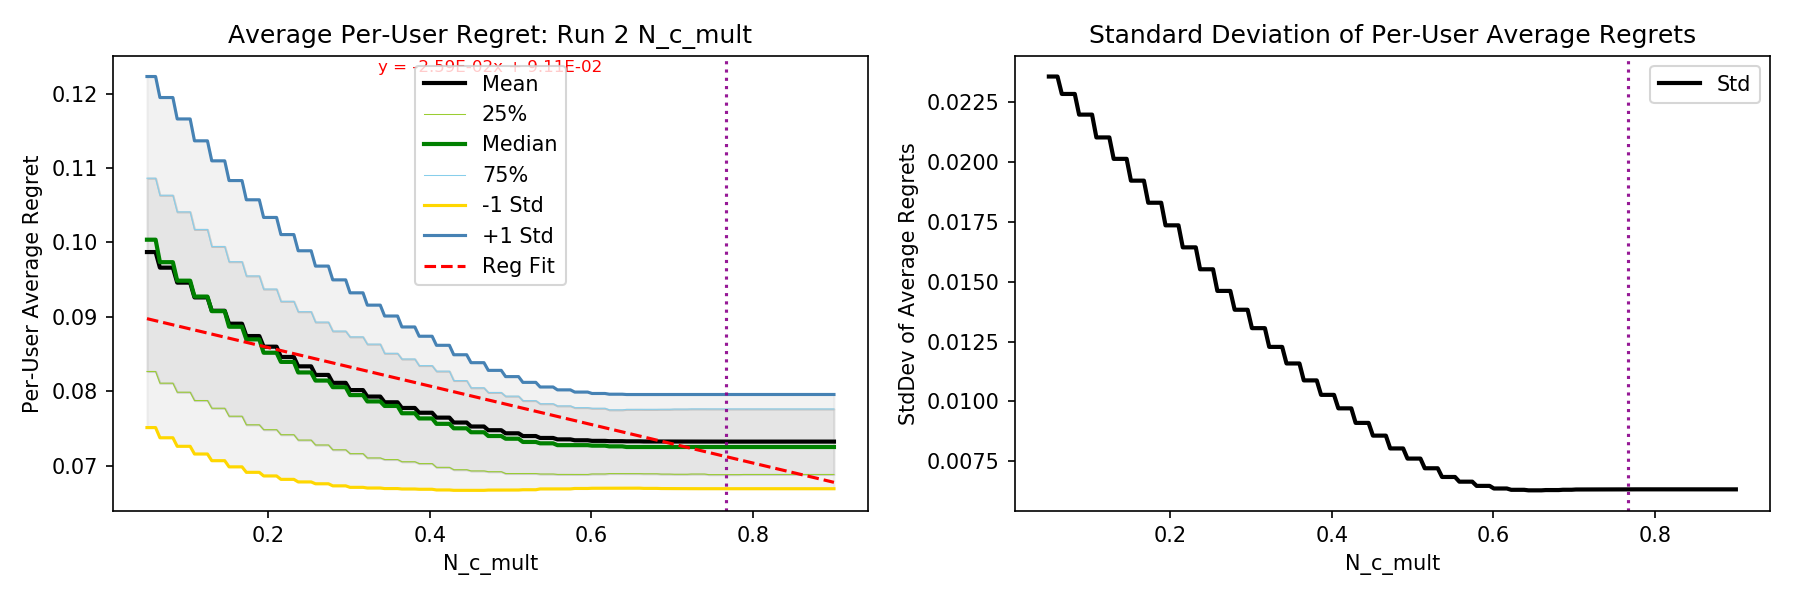
\includegraphics[width=1.1\textwidth,center]{figures/opt_param/opt_param_std_11100_N_c_mult2.png}%
	\newline
	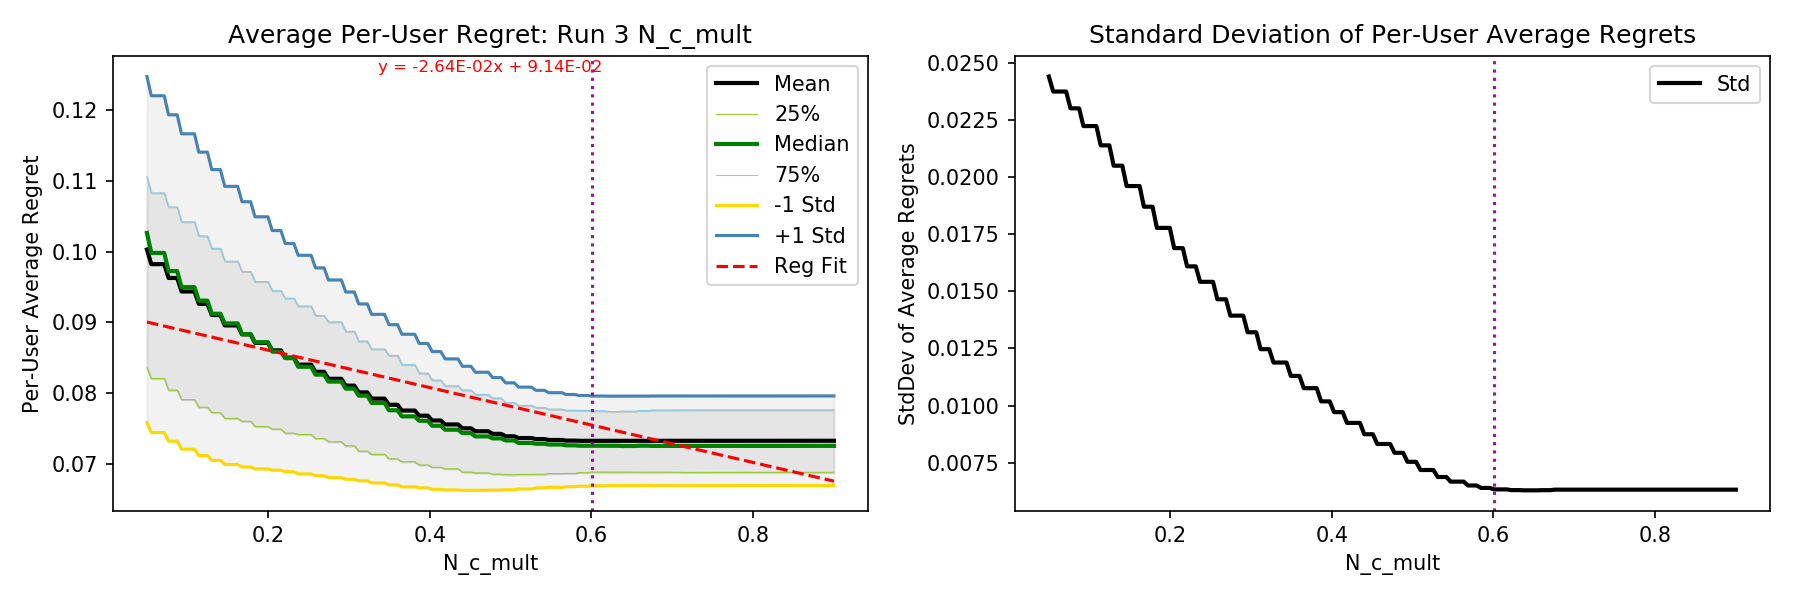
\includegraphics[width=1.1\textwidth,center]{figures/opt_param/opt_param_std_11100_N_c_mult3.png}%
	\newline
	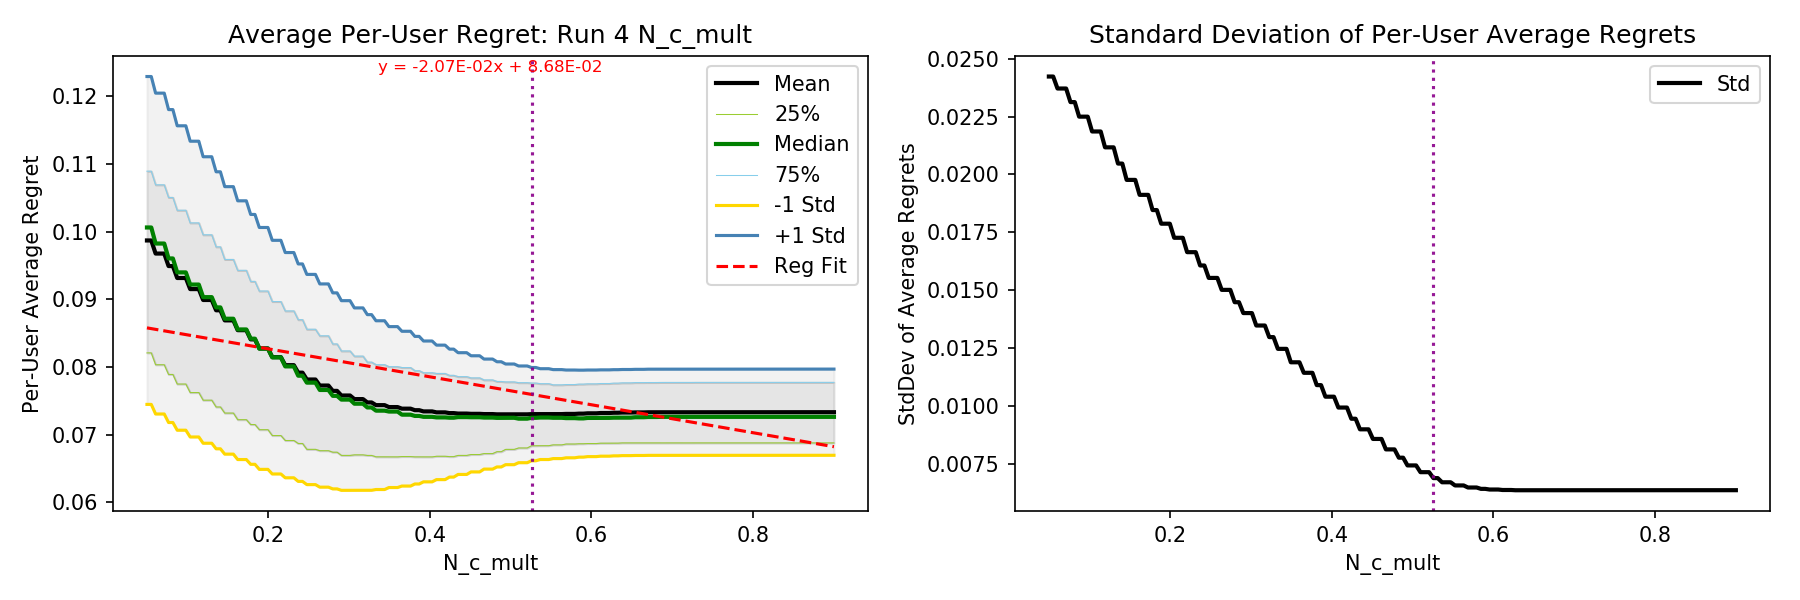
\includegraphics[width=1.1\textwidth,center]{figures/opt_param/opt_param_std_11100_N_c_mult4.png}%
	\caption{$MUER$ for Varying $\mathtt{N\_c\_mult}$, StdDev Cutoff Optimization}
	\end{figure}

	\begin{figure}[H]
	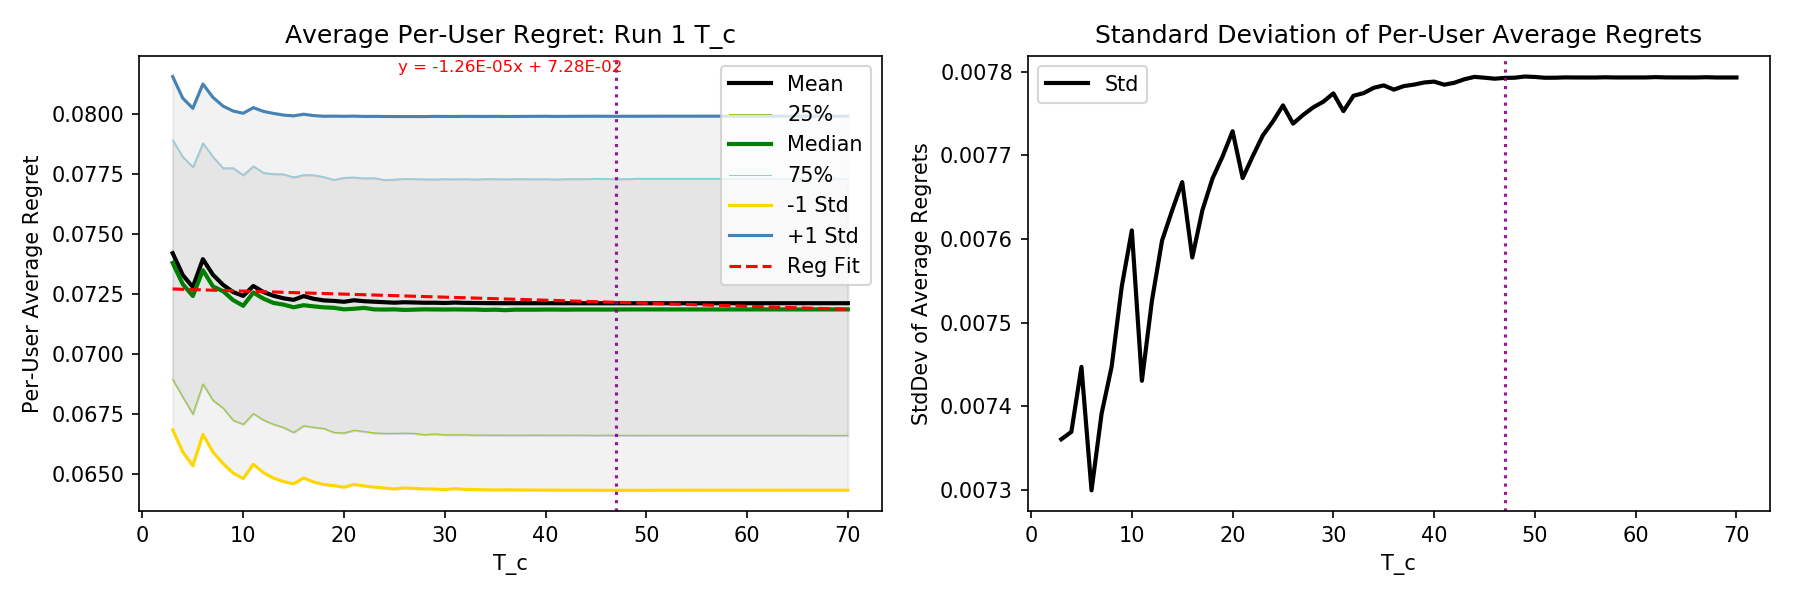
\includegraphics[width=1.1\textwidth,center]{figures/opt_param/opt_param_std_11100_T_c1.png}%
	\newline
	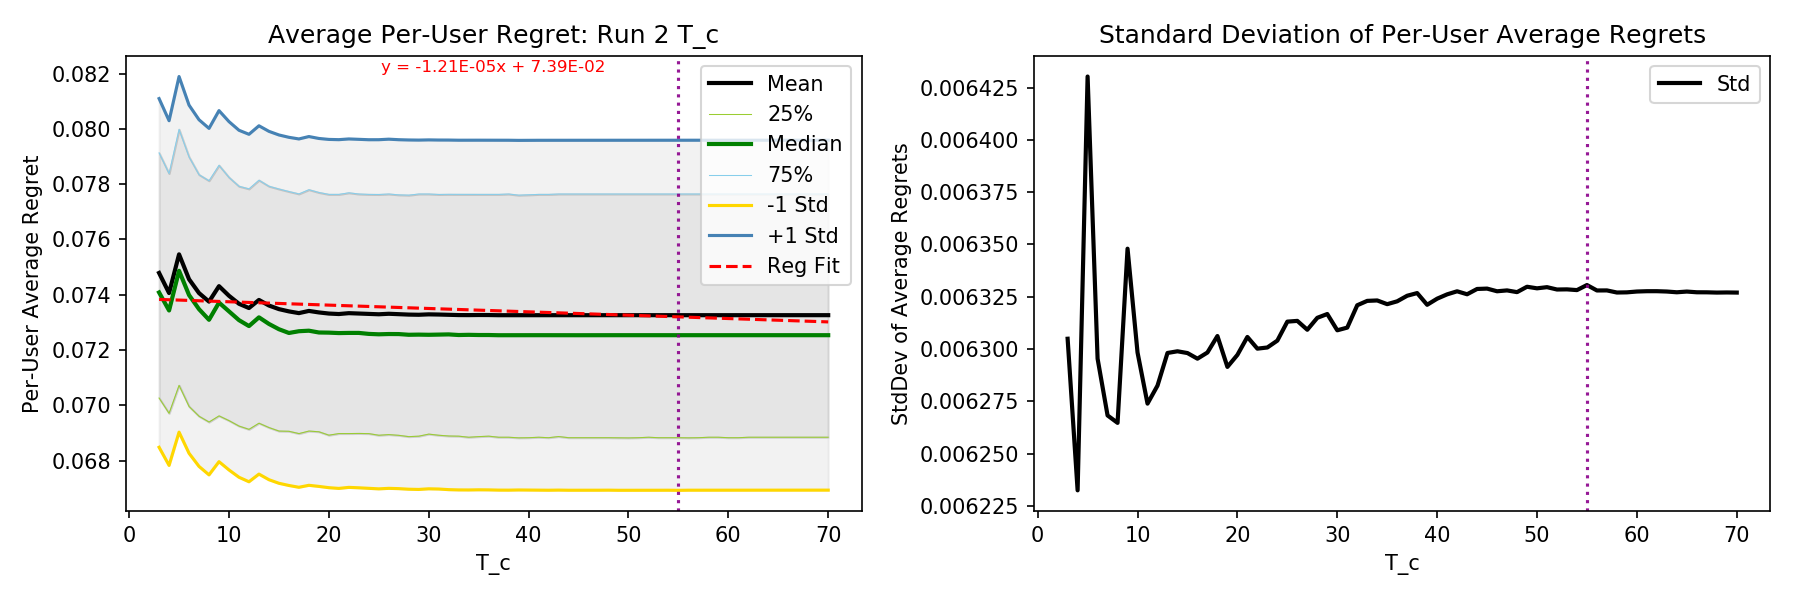
\includegraphics[width=1.1\textwidth,center]{figures/opt_param/opt_param_std_11100_T_c2.png}%
	\newline
	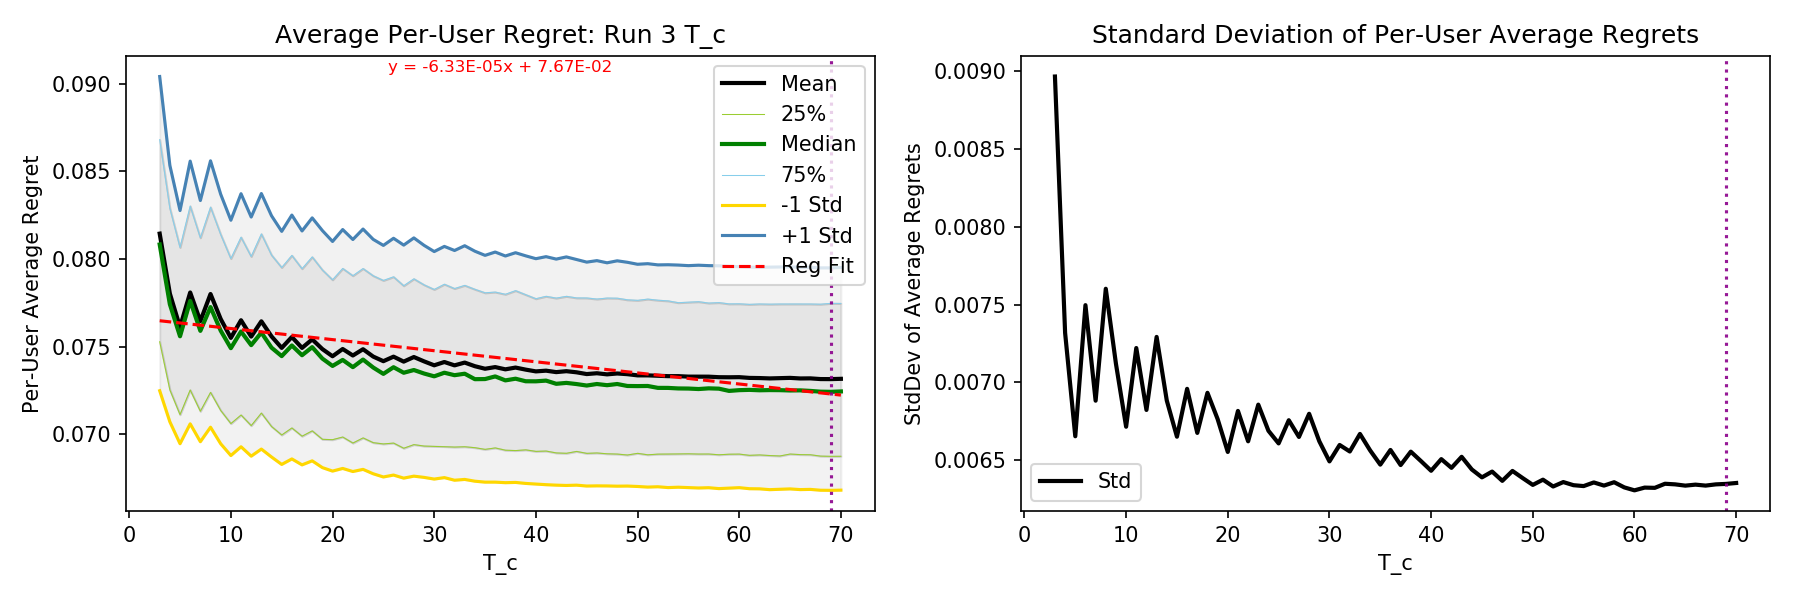
\includegraphics[width=1.1\textwidth,center]{figures/opt_param/opt_param_std_11100_T_c3.png}%
	\newline
	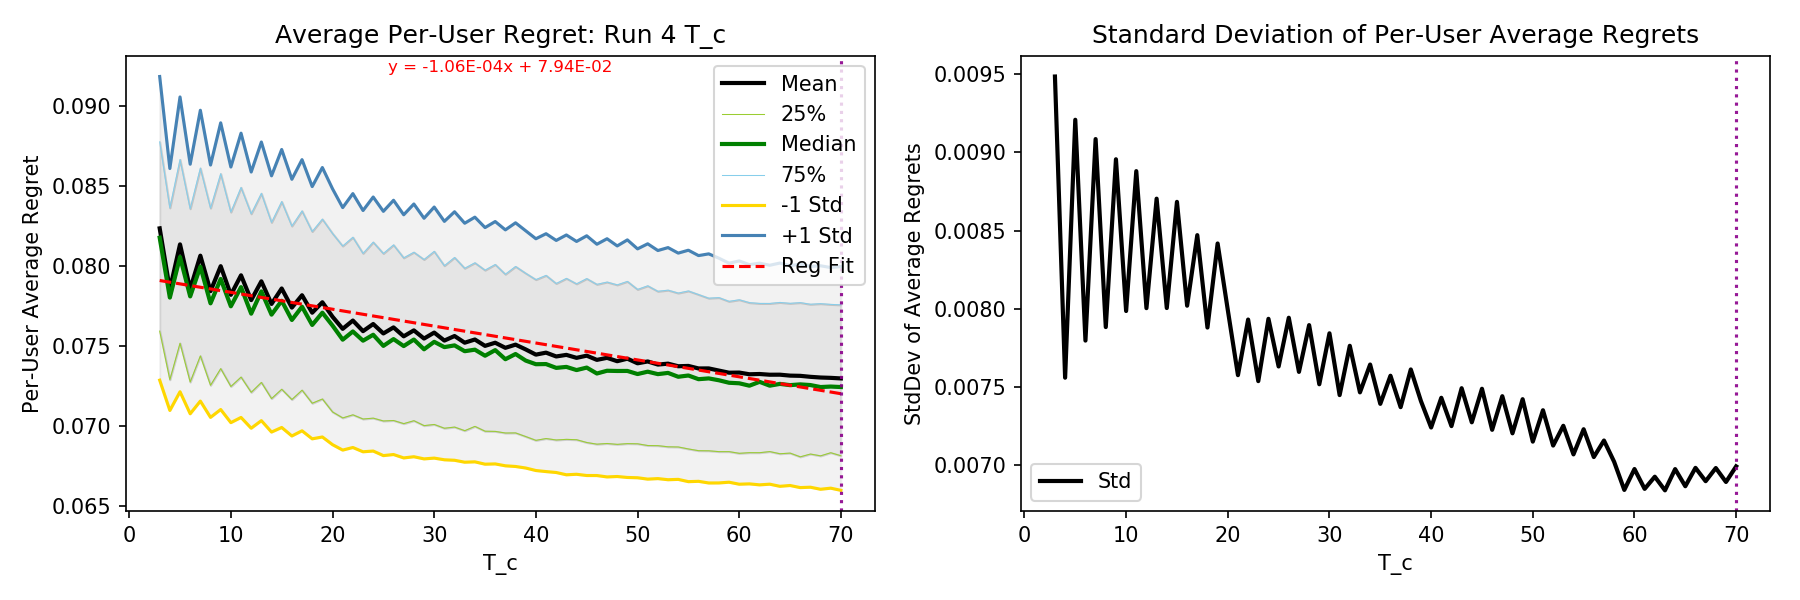
\includegraphics[width=1.1\textwidth,center]{figures/opt_param/opt_param_std_11100_T_c4.png}%
	\caption{$MUER$ for Varying $\mathtt{T\_c}$, StdDev Cutoff Optimization}
	\end{figure}

	\begin{figure}[H]
	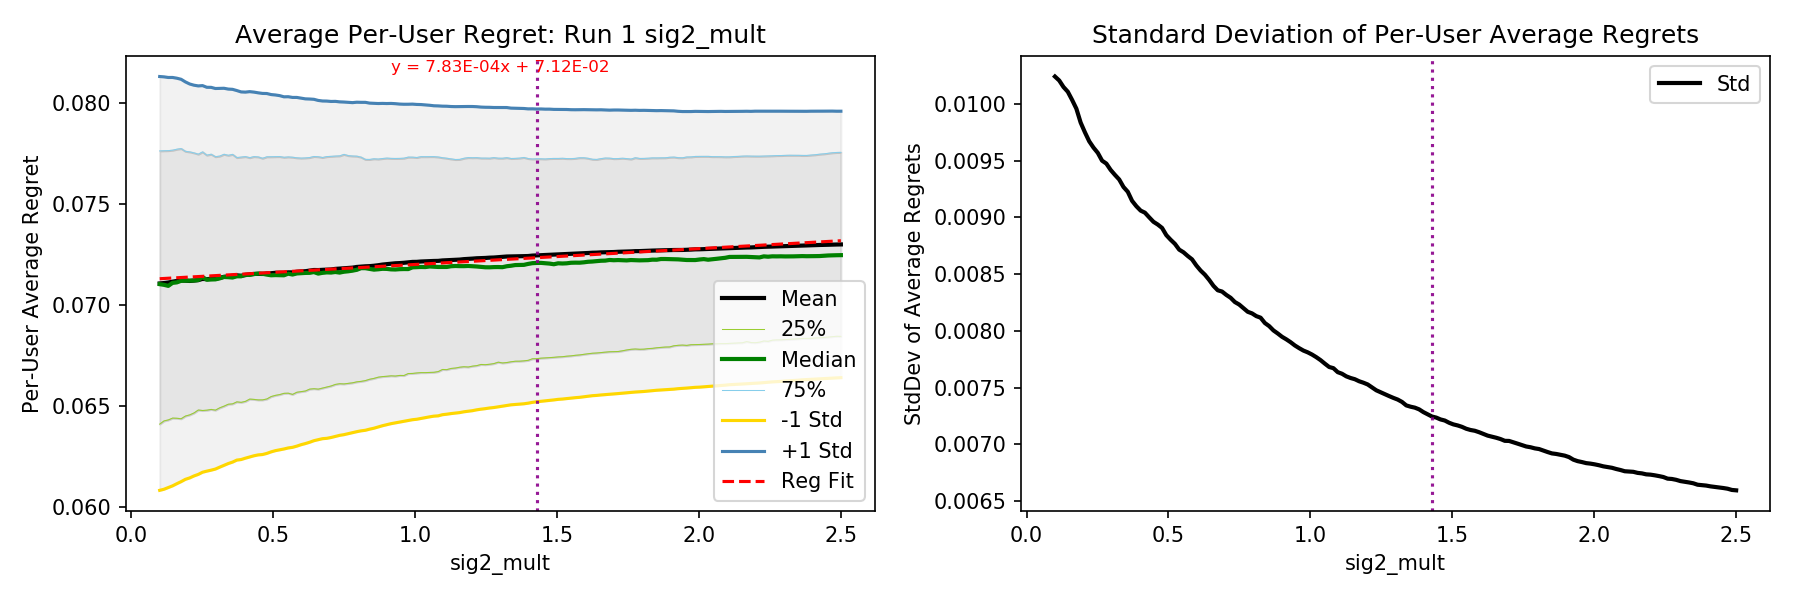
\includegraphics[width=1.1\textwidth,center]{figures/opt_param/opt_param_std_11100_sig2_mult1.png}%
	\newline
	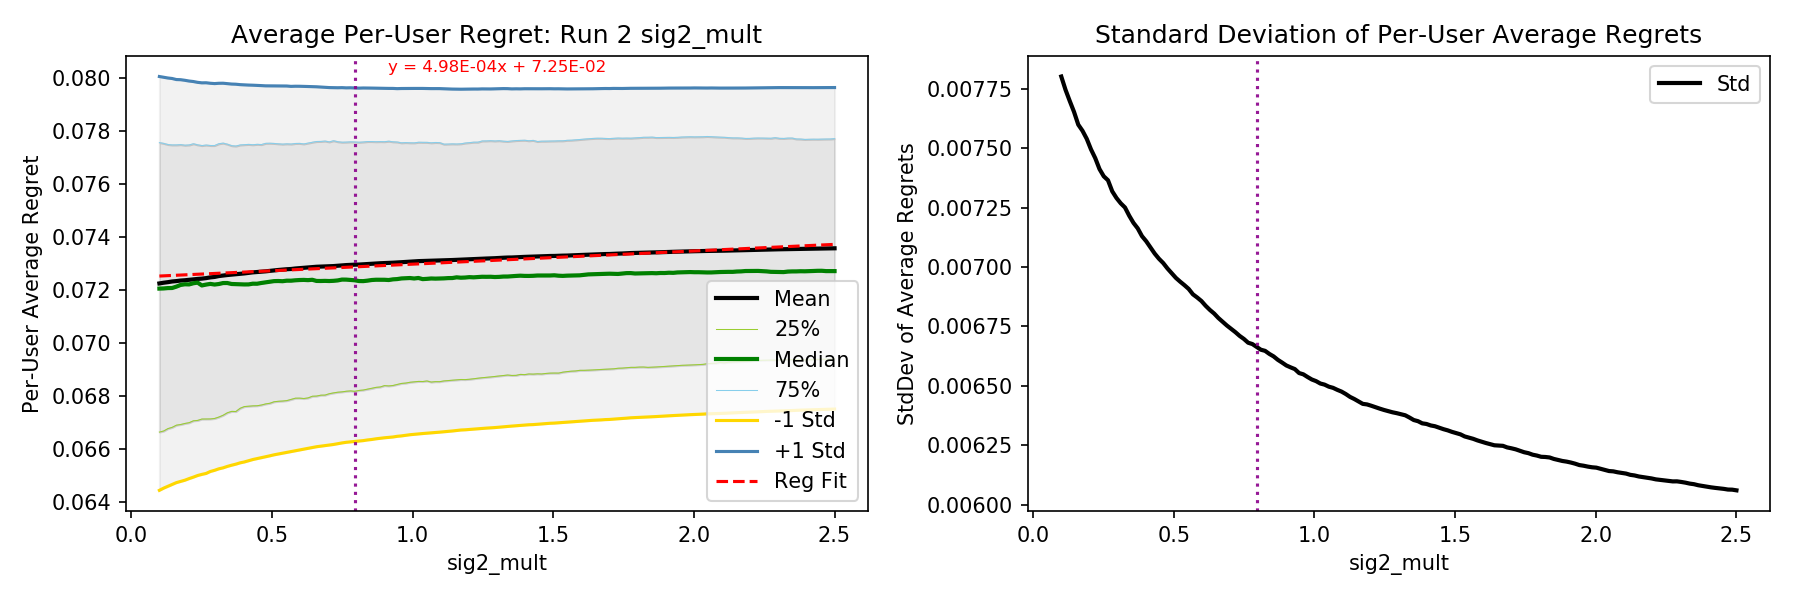
\includegraphics[width=1.1\textwidth,center]{figures/opt_param/opt_param_std_11100_sig2_mult2.png}%
	\newline
	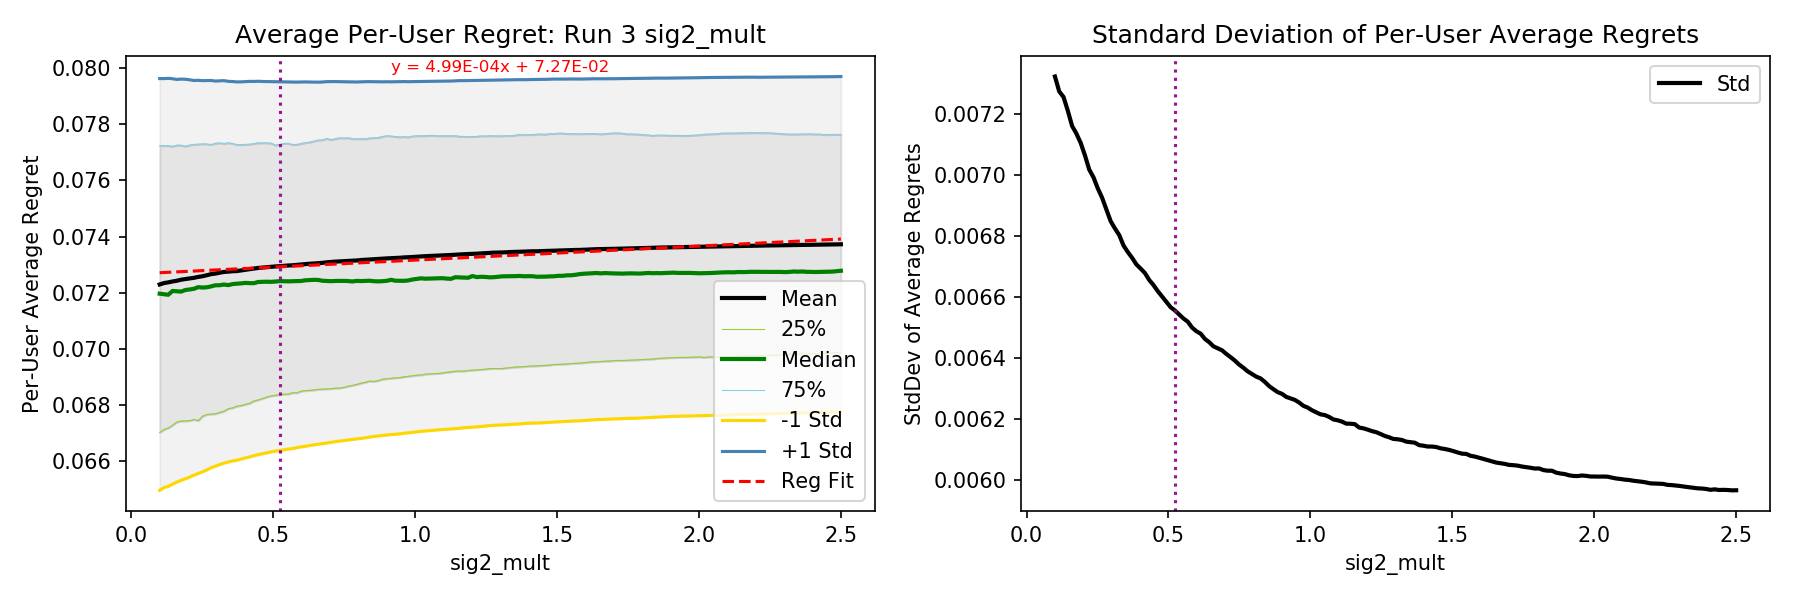
\includegraphics[width=1.1\textwidth,center]{figures/opt_param/opt_param_std_11100_sig2_mult3.png}%
	\newline
	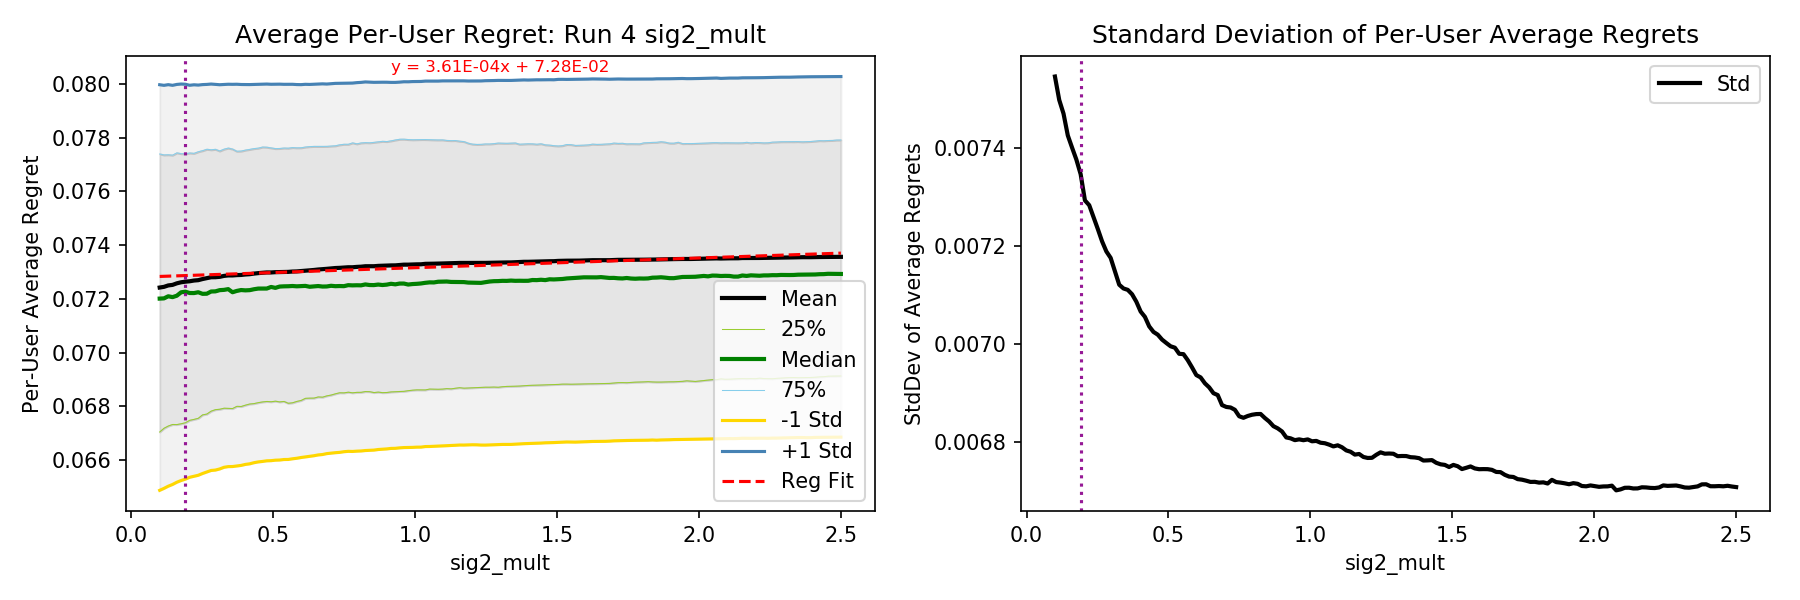
\includegraphics[width=1.1\textwidth,center]{figures/opt_param/opt_param_std_11100_sig2_mult4.png}%
	\caption{$MUER$ for Varying $\mathtt{sig2\_mult}$, StdDev Cutoff Optimization}
	\end{figure}

	\begin{figure}[H]
	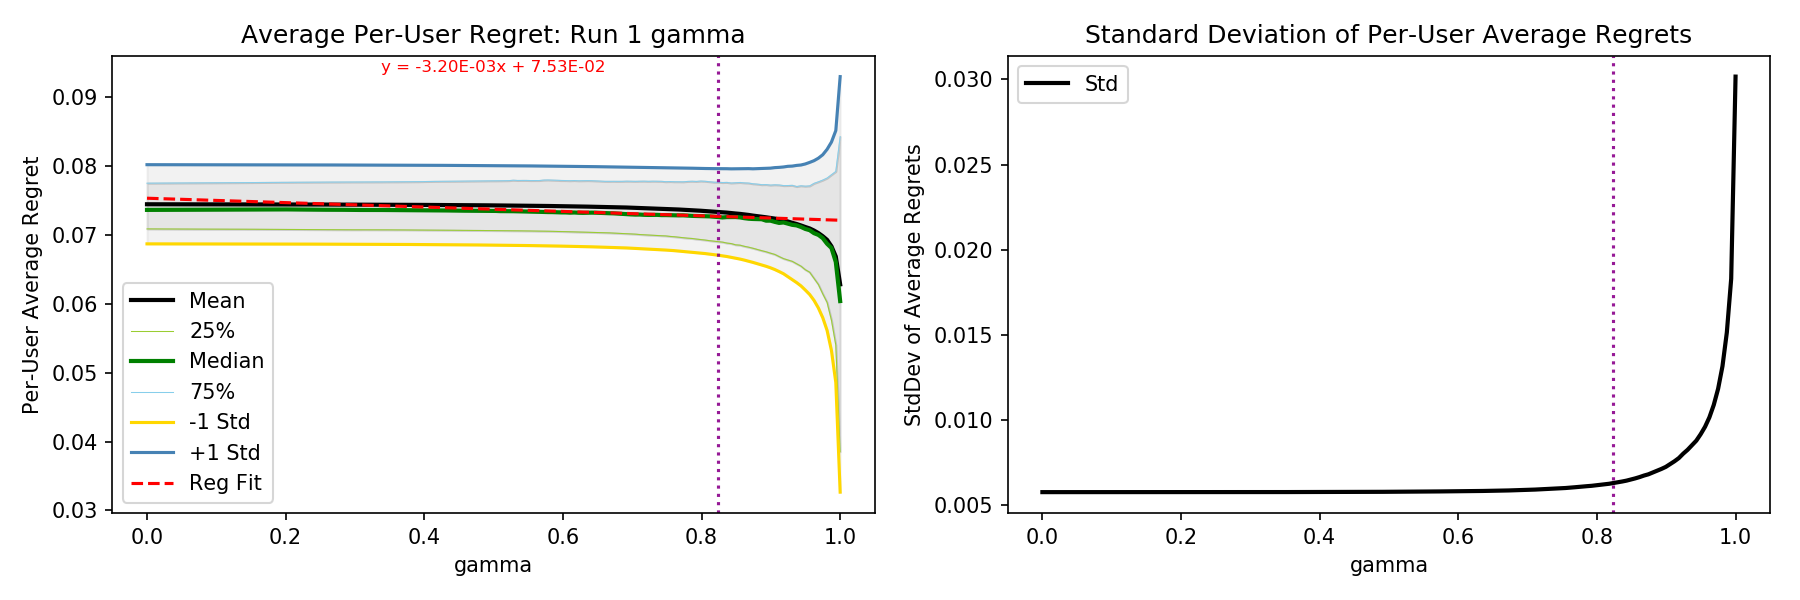
\includegraphics[width=1.1\textwidth,center]{figures/opt_param/opt_param_std_11100_gamma1.png}%
	\newline
	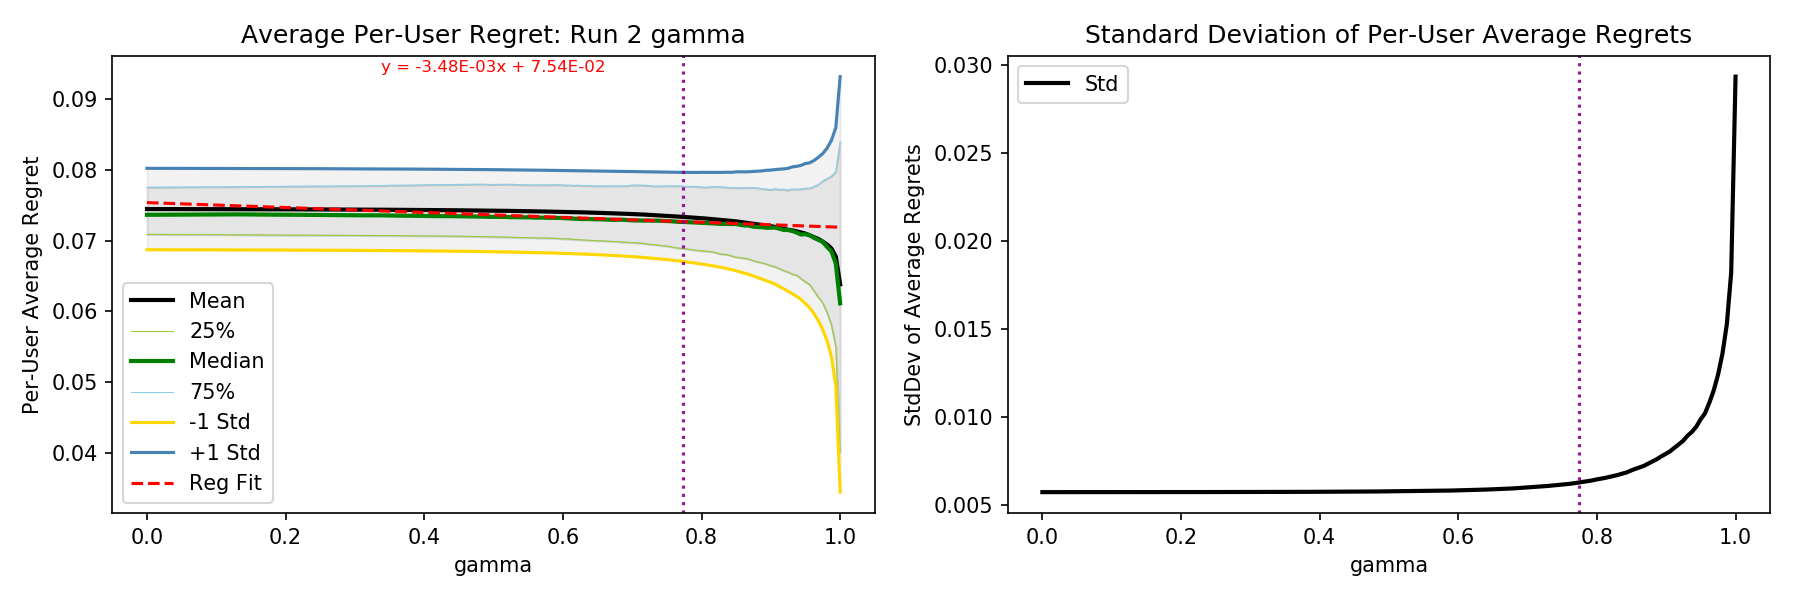
\includegraphics[width=1.1\textwidth,center]{figures/opt_param/opt_param_std_11100_gamma2.png}%
	\newline
	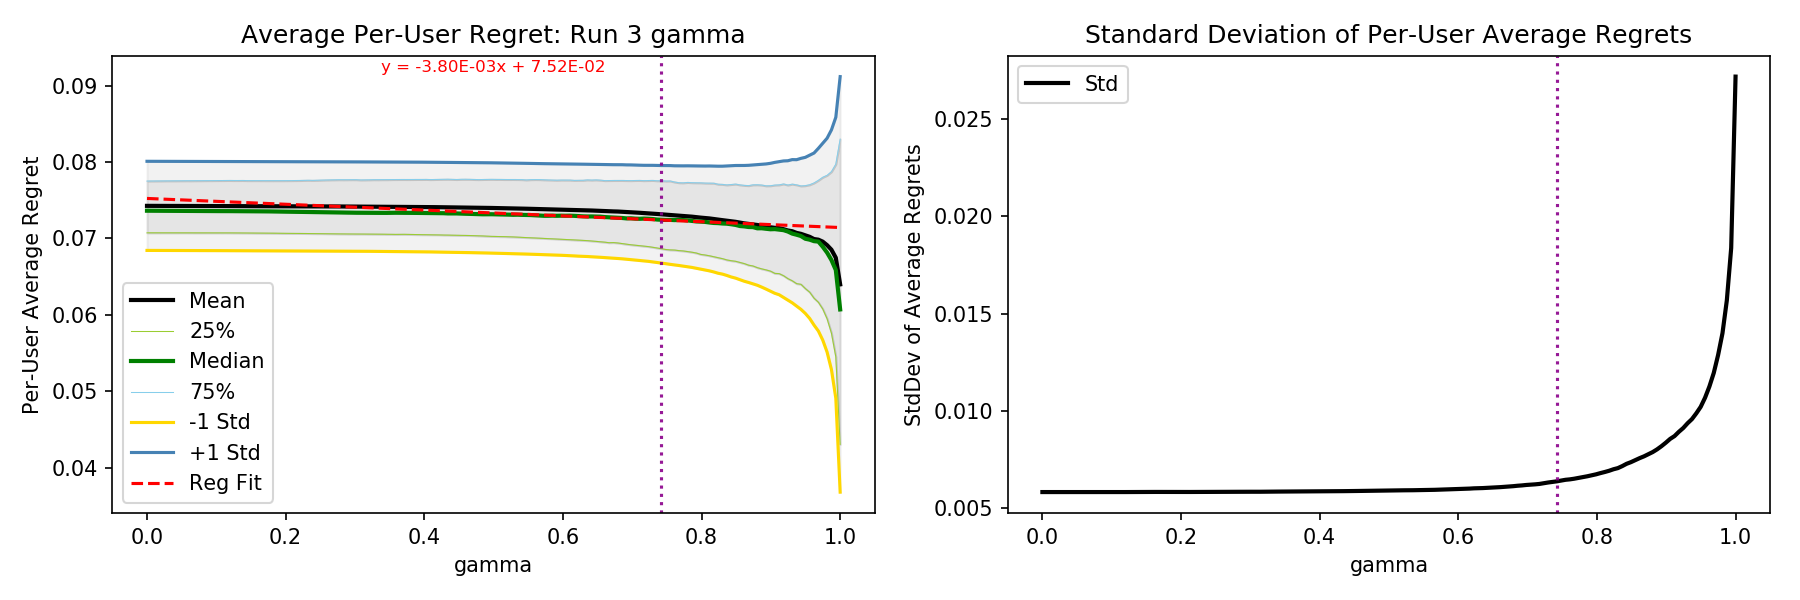
\includegraphics[width=1.1\textwidth,center]{figures/opt_param/opt_param_std_11100_gamma3.png}%
	\newline
	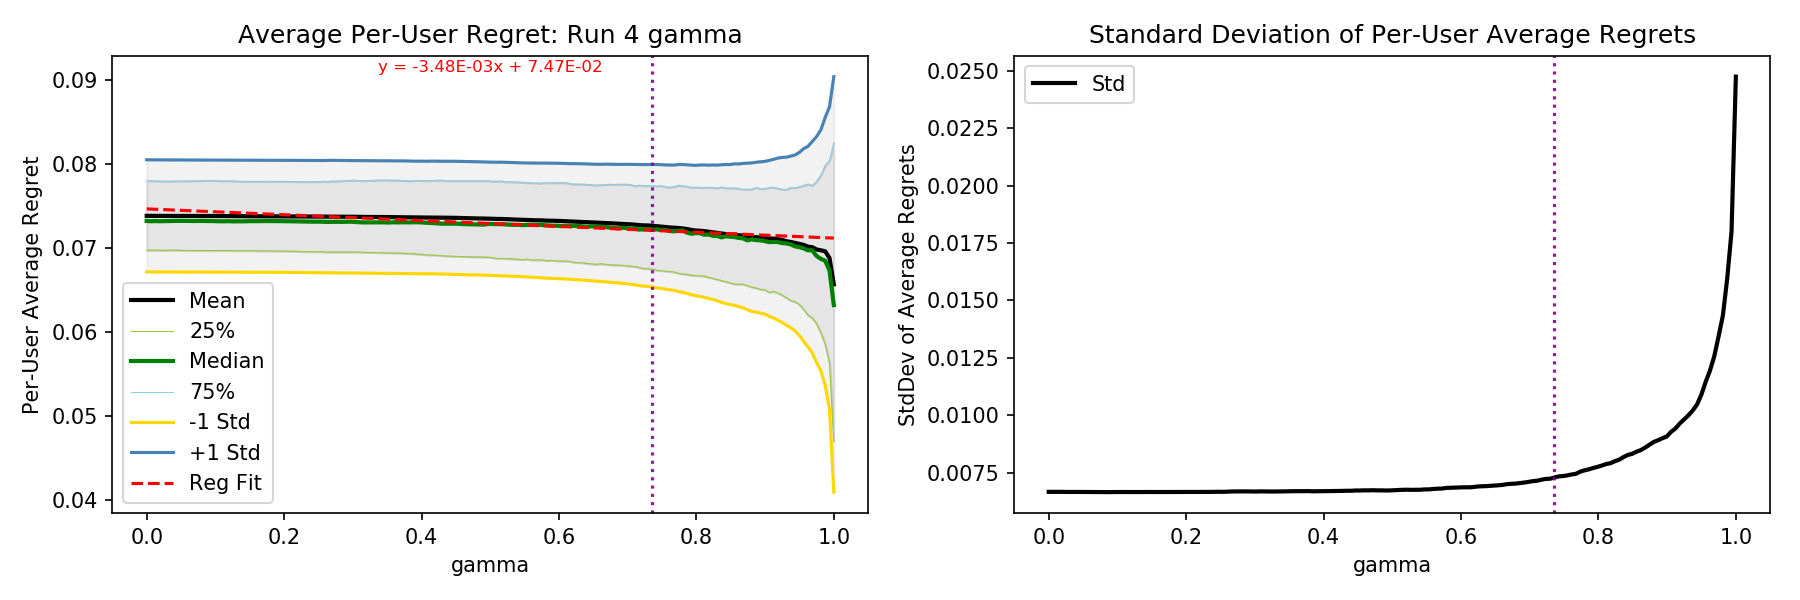
\includegraphics[width=1.1\textwidth,center]{figures/opt_param/opt_param_std_11100_gamma4.png}%
	\caption{$MUER$ for Varying $\mathtt{gamma}$, StdDev Cutoff Optimization}
	\end{figure}

	\begin{figure}[H]
	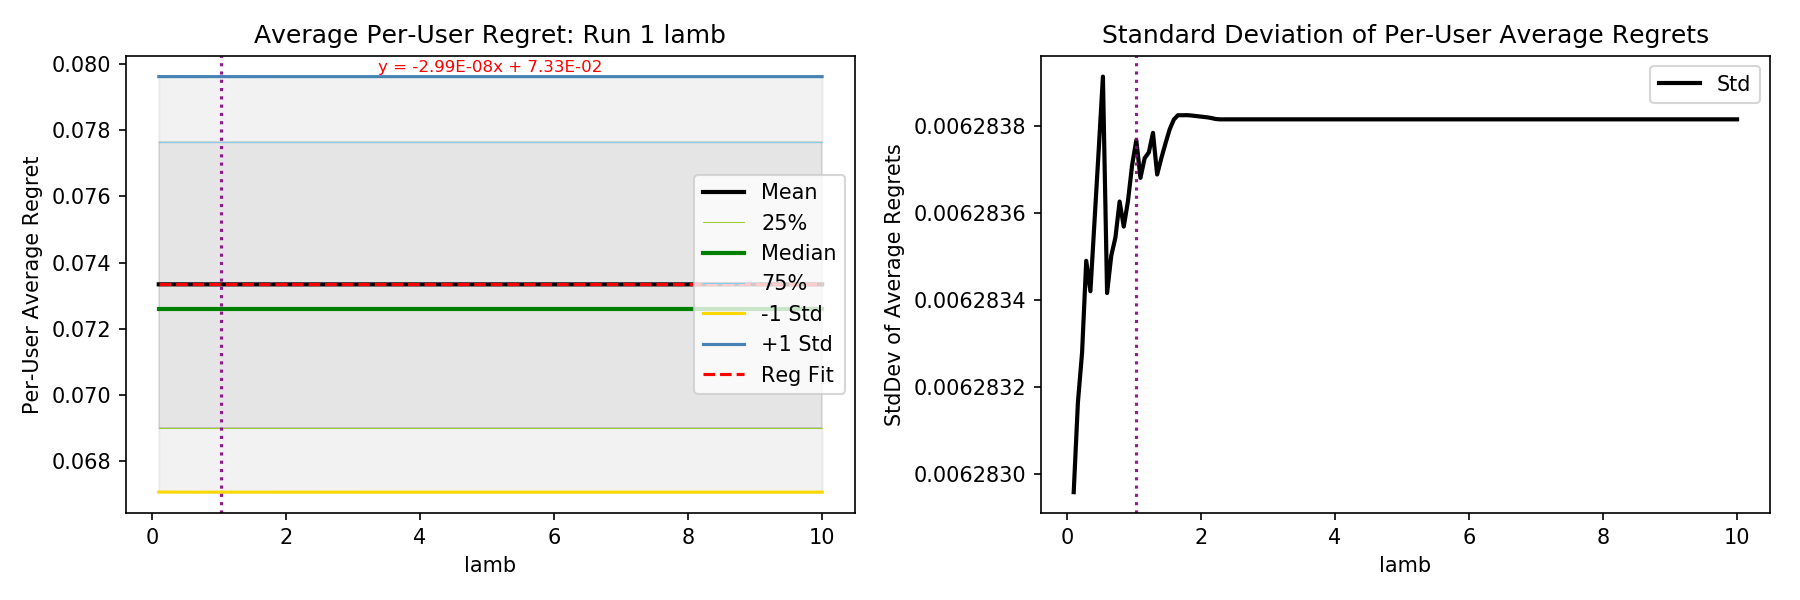
\includegraphics[width=1.1\textwidth,center]{figures/opt_param/opt_param_std_11100_lamb1.png}%
	\newline
	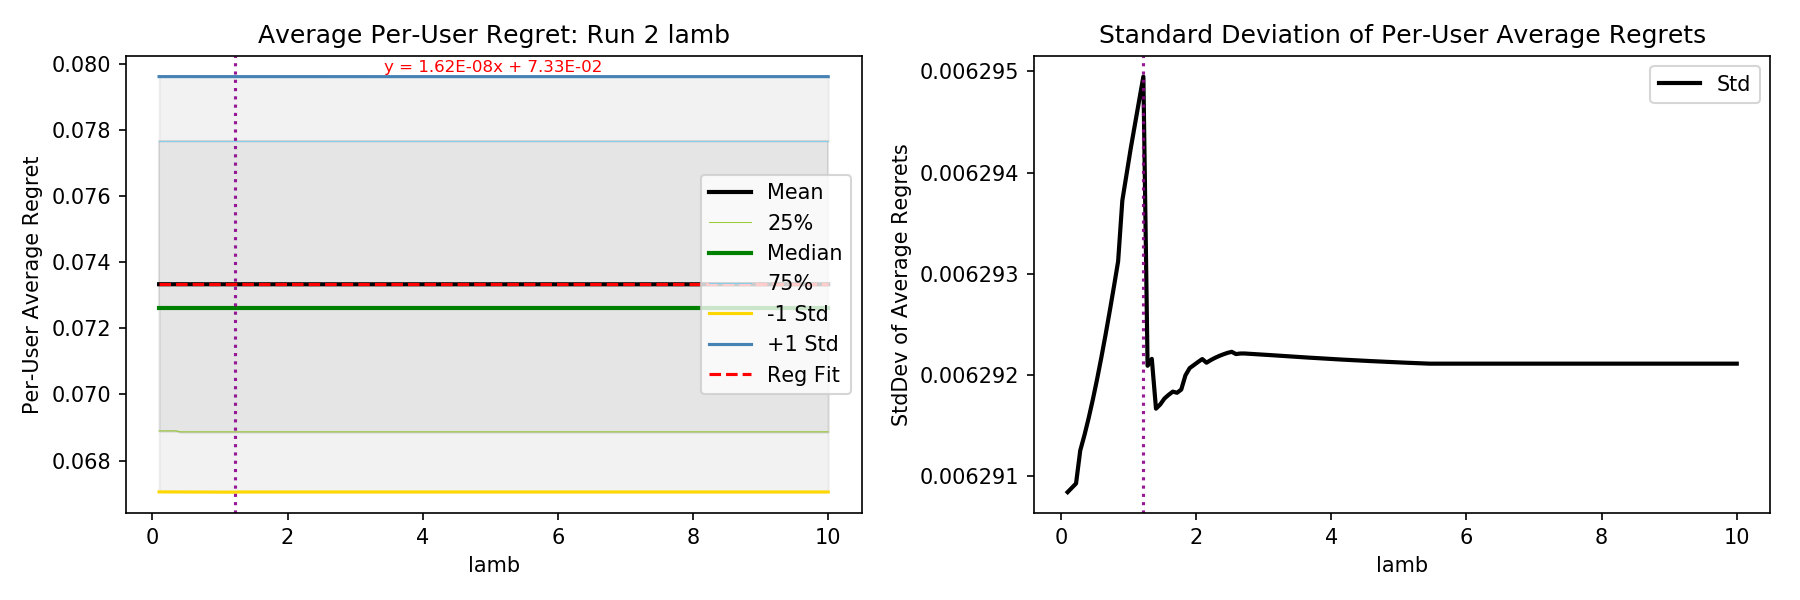
\includegraphics[width=1.1\textwidth,center]{figures/opt_param/opt_param_std_11100_lamb2.png}%
	\newline
	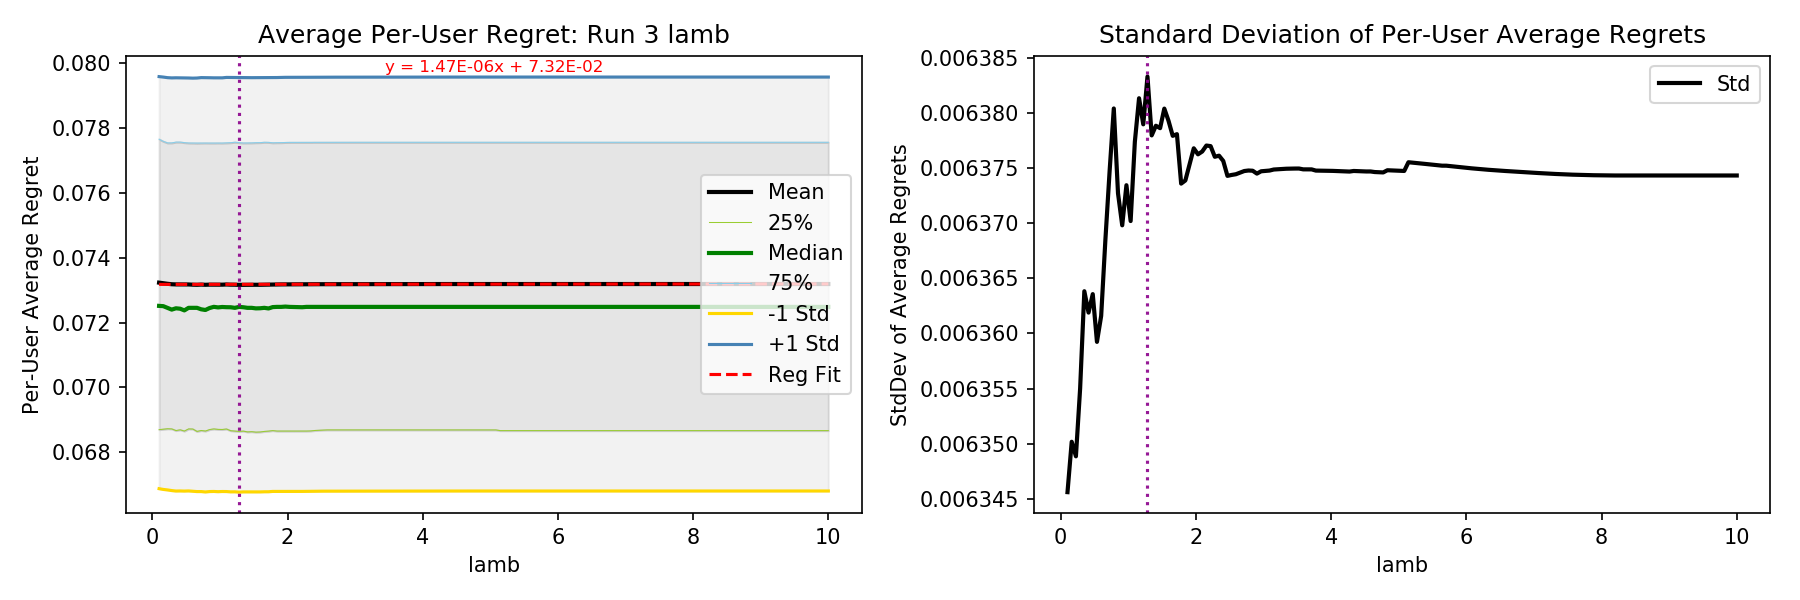
\includegraphics[width=1.1\textwidth,center]{figures/opt_param/opt_param_std_11100_lamb3.png}%
	\newline
	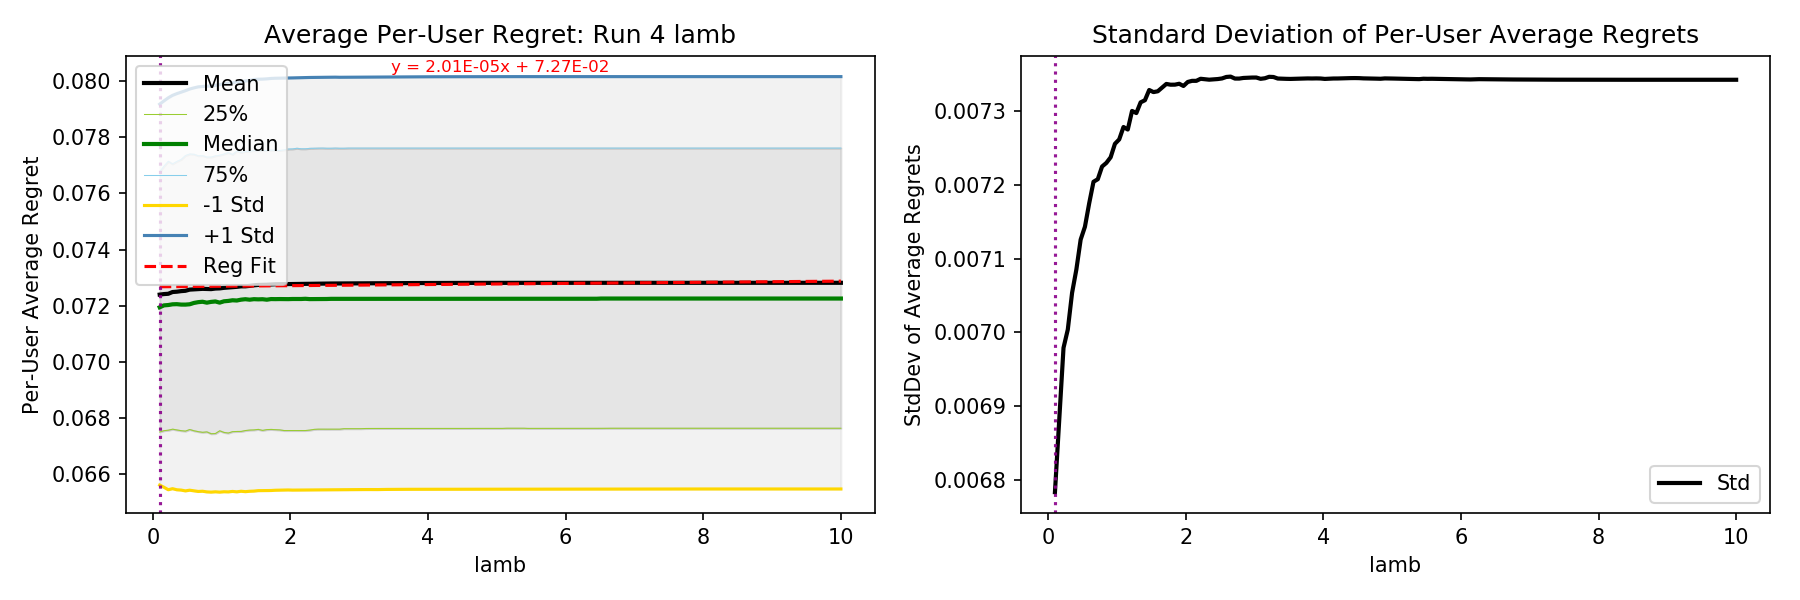
\includegraphics[width=1.1\textwidth,center]{figures/opt_param/opt_param_std_11100_lamb4.png}%
	\caption{$MUER$ for Varying $\mathtt{lamb}$, StdDev Cutoff Optimization}
	\end{figure}

	\begin{figure}[H]
	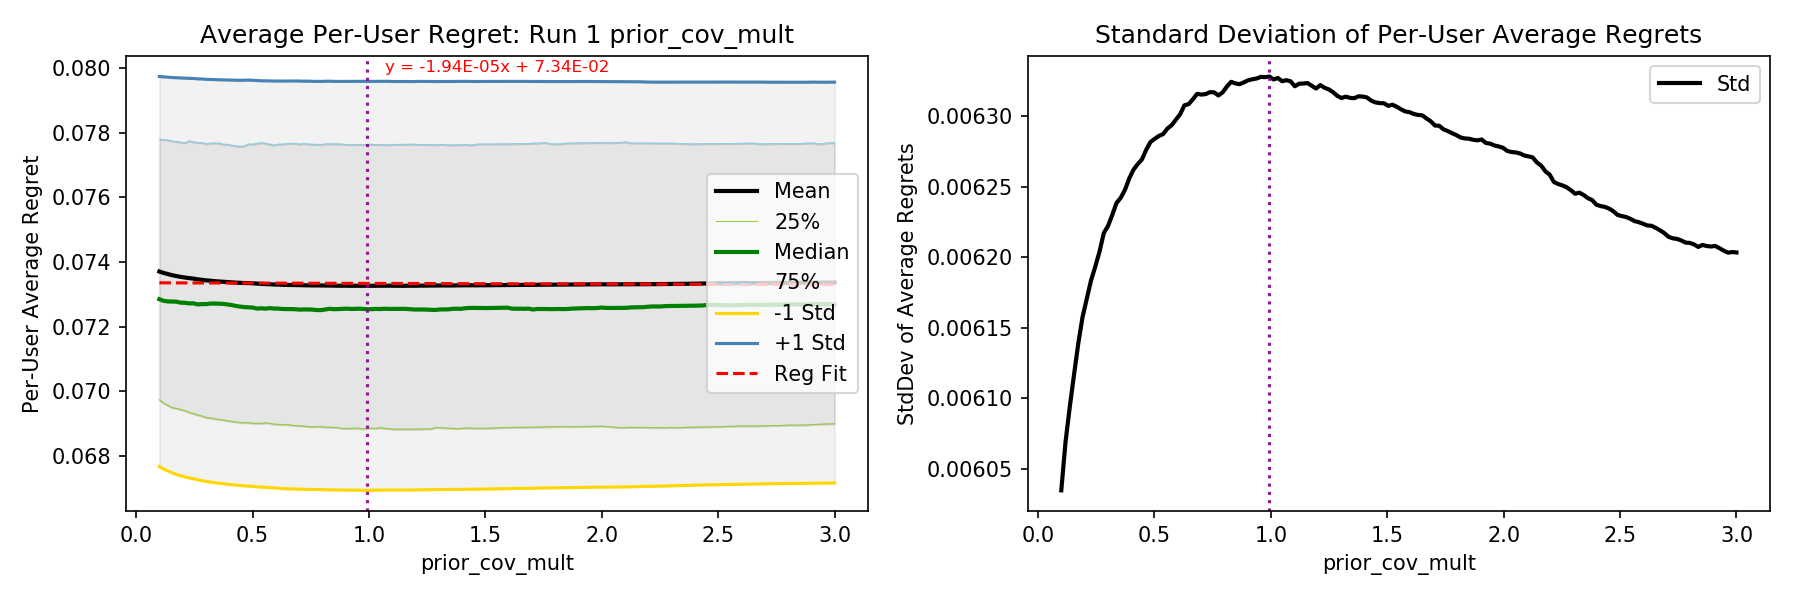
\includegraphics[width=1.1\textwidth,center]{figures/opt_param/opt_param_std_11100_prior_cov_mult1.png}%
	\newline
	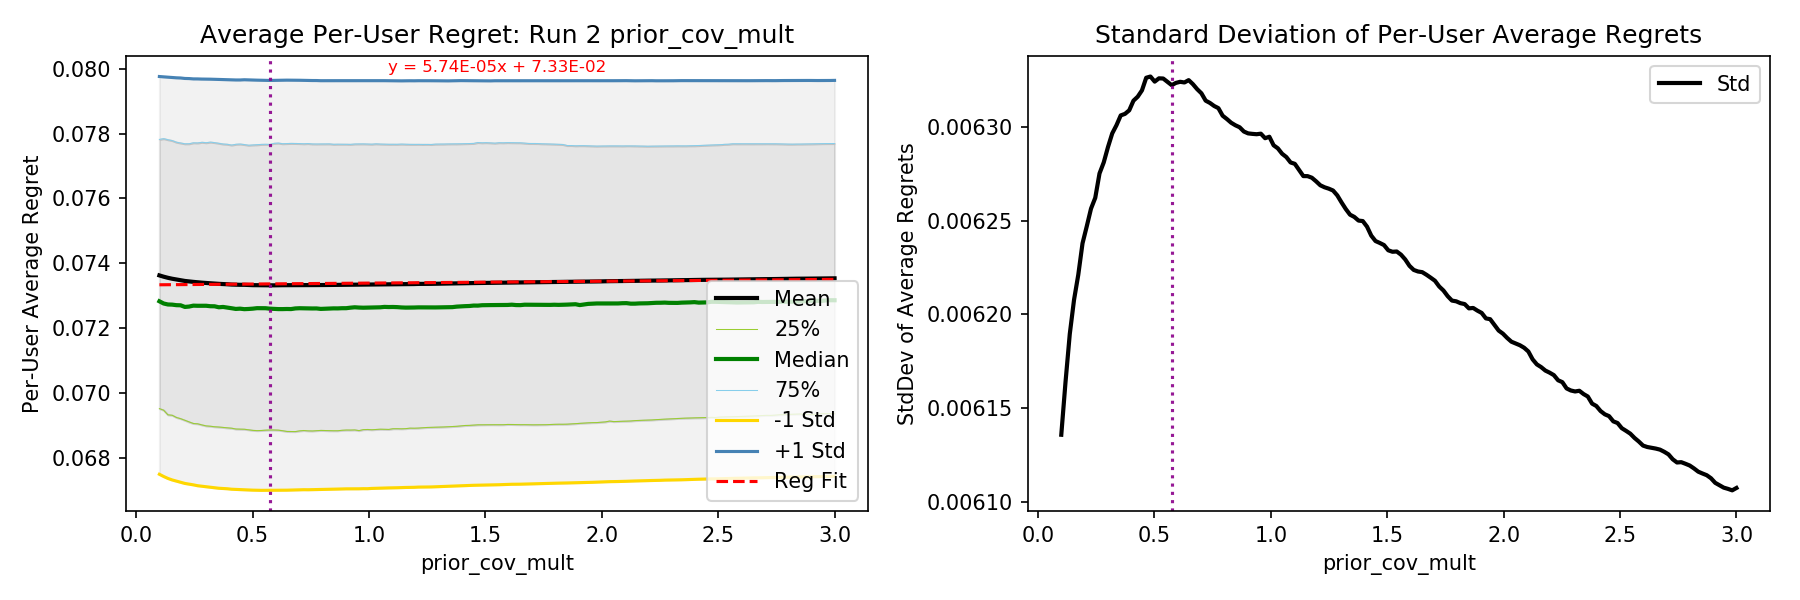
\includegraphics[width=1.1\textwidth,center]{figures/opt_param/opt_param_std_11100_prior_cov_mult2.png}%
	\newline
	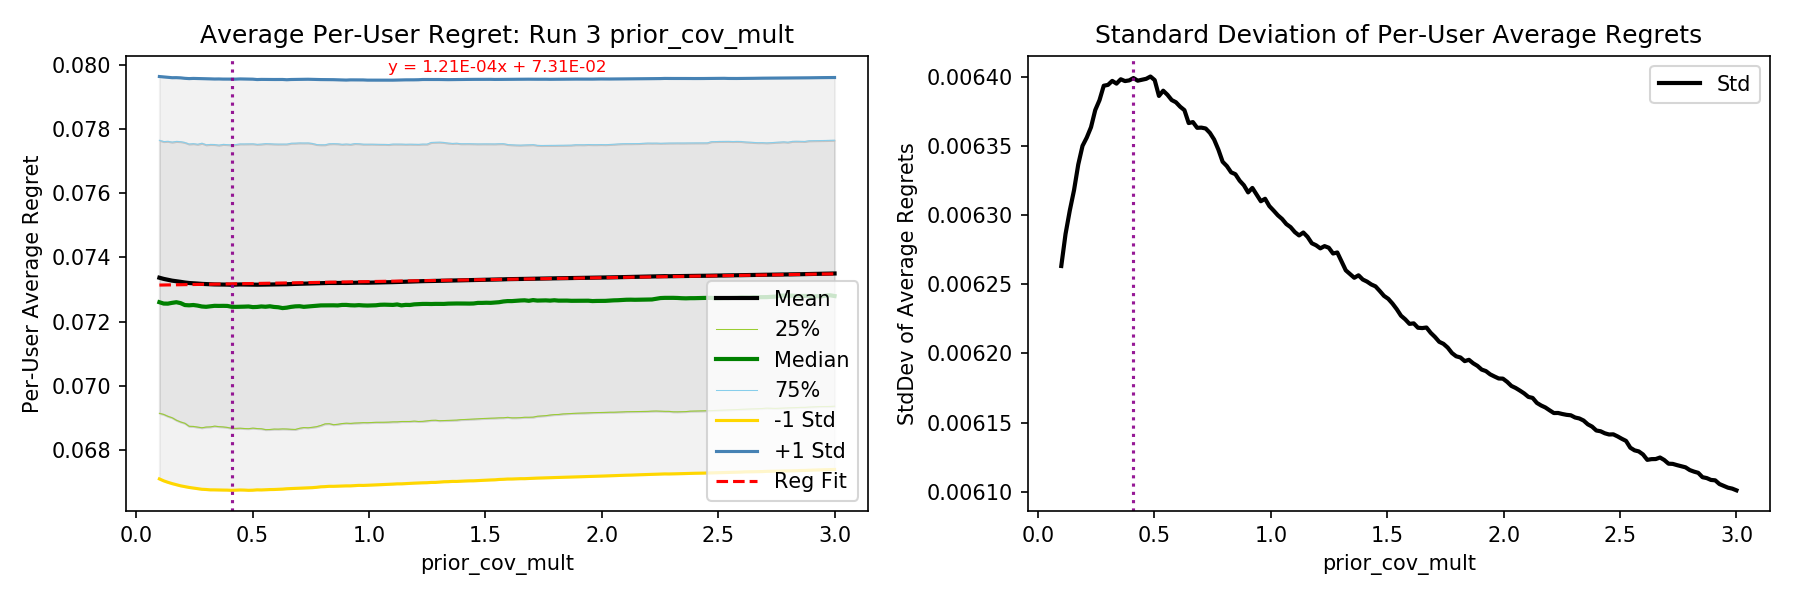
\includegraphics[width=1.1\textwidth,center]{figures/opt_param/opt_param_std_11100_prior_cov_mult3.png}%
	\newline
	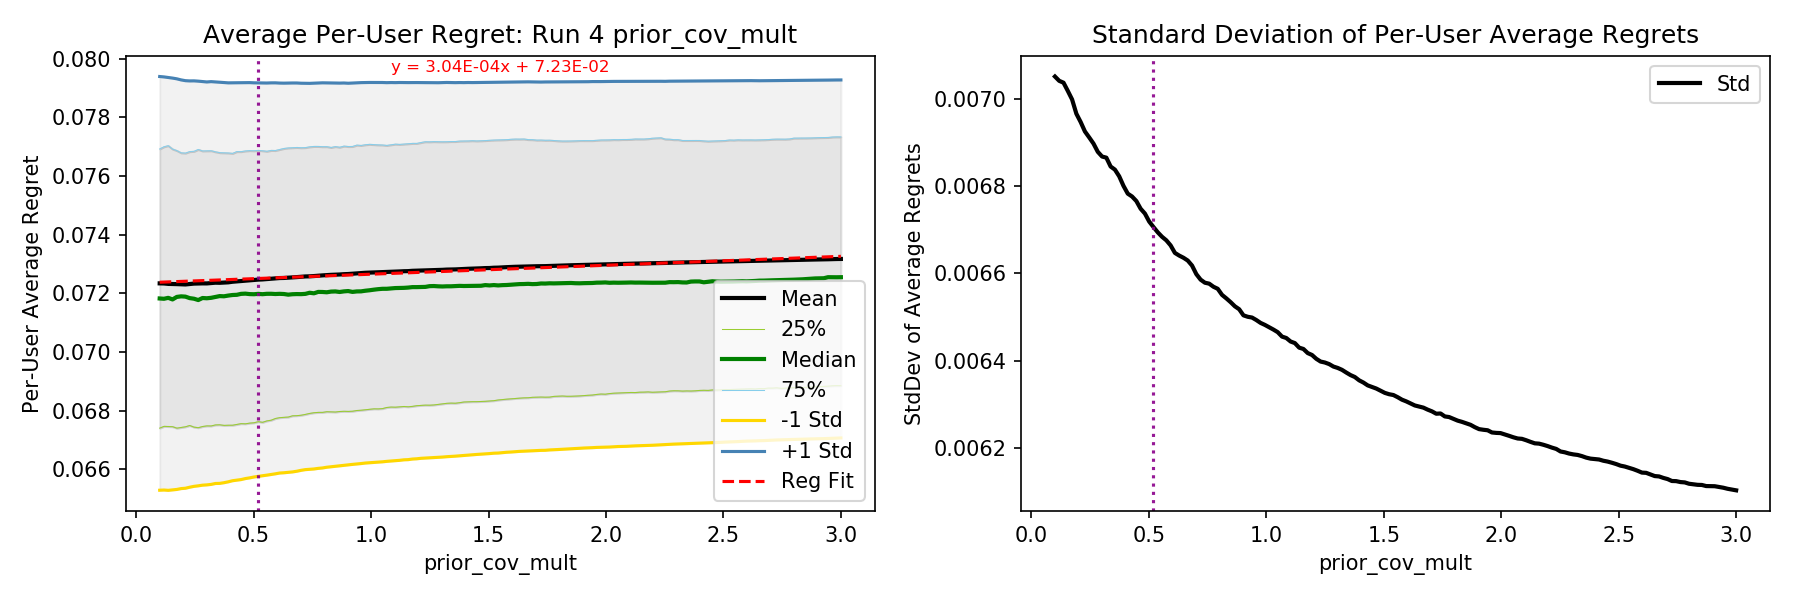
\includegraphics[width=1.1\textwidth,center]{figures/opt_param/opt_param_std_11100_prior_cov_mult4.png}%
	\caption{$MUER$ for Varying $\mathtt{prior\_cov\_mult}$, StdDev Cutoff Optimization}
	\end{figure}
	\fi


​

%%%%%%%%%%%%%%%%%%%%%%%%%%%%%%%%%%%%%%%%%%%%%%%%%%%%%%%%%%%%%%%%